\documentclass[a4paper]{article}

\usepackage[latin1]{inputenc}
\usepackage{graphicx}
\usepackage{amsthm} 
\usepackage{amsmath}
\usepackage{txfonts}
\usepackage{MnSymbol}
\usepackage{float}
\usepackage{subfigure}
\usepackage[toc,page]{appendix} 
\usepackage{textcomp}

\begin{document}

\def\ci{\perp\!\!\!\perp}
\newcommand\independent{\protect\mathpalette{\protect\independenT}{\perp}} 
\def\independenT#1#2{\mathrel{\rlap{$#1#2$}\mkern2mu{#1#2}}} 

\setlength{\parskip}{1.5ex} % 1ex plus 0.5ex minus 0.2ex}
\setlength{\parindent}{0pt}
\newcommand{\definition}[1]{\textit{\textbf{#1}}}
\newenvironment{theorem}[1]{\textbf{#1}$\quad$\begin{itshape}}{\end{itshape}}

\author{Ait-taleb nabil}
\title{Génération de jeux de données multicritères réalistes à partir de réseaux Bayésiens}

\maketitle

\tableofcontents

\newpage

\section{Introduction}



L\textquotesingle aide à la décision est l\textquotesingle ensemble des techniques permettant, pour une personne donnée, d\textquotesingle opter pour la meilleure prise de décision possible par rapport à certaines alternatives évaluées sur plusieurs critères.
Par exemple le problème consistant à acheter une voiture est un problème multicritère où l'ensemble des voitures jouent le rôle d'alternatives.
 Le choix d'un décideur pourra dépendre des critères tel que le prix, le confort ou  la tenue de route du véhicule etc.
Le principe est alors de ranger les alternatives en construisant un modèle qui intègre à la fois les évaluations objectives des voitures  et les préférences du décideur.
Il existe différentes méthodes pour évaluer la meilleur prise de décision tel que l\textquotesingle utilisation d\textquotesingle une fonction à valeur ajoutée, la méthode ELECTRE, la méthode Saaty  etc.

Quand on propose de nouvelles méthodes on souhaite tester leurs  propriétés. Pour que les propriétés soit statistiquement significatives, nous devons utiliser de grand jeux de données, or les jeux de données rencontrées dans les problèmes d\textquotesingle aides à la décision sont de petites tailles. Il faut alors les créer artificiellement. 

Nous pourrions générer les jeux aléatoirement mais les résultat serait peu réaliste. En effet dans les jeux de données multicritères réalistes, nous retrouvons des corrélations ; par exemple la voiture la plus cher est souvent la plus rapide et  la plus confortable.
L\textquotesingle objectifs final de ce travail est alors de générer des grands jeux de données corrélées qui ressemblent à des données multicritères réaliste.




\textbf{Comment faire ?}

\begin{itemize}
\item On pourrait analyser la matrice des corrélations et puis générer aléatoirement des variables corrélées deux à deux  mais il est difficile de reconstituer  totalement la matrice de départ.


\item L\textquotesingle analyse en composante principale donne aussi une indication sur les dépendances mais elle  ne donne aucune piste pour générer des valeurs.
Dans le cadre de ce travail, nous opterons de générer nos jeux de données multicritèreres à l'aide des réseaux bayésiens.

\end{itemize}
Les réseaux Bayésiens possèdent de nos jours  un champ d'application assez vaste, par exemple:

\begin{enumerate}
  \item Diagnostic médical et industriel.
  \item L'analyse de risque.
  \item La détection de spam.
  \item Le data mining.
  \item L'intelligence artificielle.
\end{enumerate}




\newpage
Le modèle mathématique attribué à un jeux de données expliquant les dépendances inter-critères  sera une application d'un ensemble de critères $C_{i=1..m}$ via un système relationnel du type:

\[
\{C_{1},C{2},...,C_{m}\}\Longrightarrow\left\lbrace 
\begin{array}{lcl} 
(C_{i}\ci C_{j})_{i\neq j}\\
  (C_{i} \not\ci C_{j})_{i\neq j}\\
(C_{i}\ci C_{j}|\bigcup_{k} C_{k})_{i\neq j \neq k}\\  
(C_{i}\not\ci C_{j}|\bigcup_{k} C_{k})_{i\neq j \neq k}\\  
\end{array}\right.
\]

Ce modèle sera appelée \textit{modèle de dépendance $\not\ci$ et d'indépendance $\ci$}

Une représentation Bayésienne sera alors associée aux relations.
Nous pourrons alors générer des jeux de données et la validation des données  se fera de manière statistique.

Ce travail comprend 5 grandes sections:

\begin{enumerate}

  \item Une introduction théorique sur les réseaux bayésiens: nous exposerons dans ce point les éléments fondamentaux concernant les réseaux bayésiens permettant de mener à bien la compréhension du travail.

  \item Une section concernant l'apprentissage: il y sera brièvement  exposé les deux métriques utilisées à postériori:
\begin{itemize}	
    \item BIC-Gaussienne.

   \item BGE métrique.

\end{itemize}
  \item Une section sur l'analyse de données:
    nous présenterons les  trois outils statistiques (ACP 2D, test d'hypothèse Student et le diagramme en boîte ) que nous utiliserons dans la validation de nos jeux de données.



  \item Apprentissage sur des données réalistes:

    Nous étudierons la légitimité des méthodes d'apprentissages décrites dans la deuxième section.
    Deux méthodes de bruitages agissant directement sur le jeu de données brut seront utilisée.
    Ceci permettra de tester la robustesse du réseau appris et de décorréler nos critères.

  \item Une section traitera la création des jeux de données généré à partir de réseaux bayésiens:

    A partir d'une modélisation,
    nous serons amenés à générer des données.
    On testera la vraisemblance des résultats par rapport à la modélisation mathématique de départ et le réalisme des données artificiels par rapport aux données réalistes.

\end{enumerate}
   
Les traitements informatiques seront faits à l'aide du programme R où nous utiliserons les librairies "bnlearn" et "FactoMineR" .
  
\newpage


\subsection{Définition d'un réseaux Bayésien}

Un \definition{réseaux Bayésien} B(X,$\Theta$)  est un Graphe non-orienté acyclique  où les noeuds représentent des variables aléatoires $x_{i=1...n} \in X$
auxquelles nous attribuons  un ensemble de paramètres $\theta_{i=1,...,n} \in \Theta$,
correspondant aux probabilités conditionnelles des variables courantes étant donnés les parents.

Ce réseaux est représenté par  une loi de probabilité  $P$:

\begin{center}
$X\ci_{B}Y|Z\Longrightarrow X\ci_{B}Y|Z$
\end{center}


\subsection{Théorème de factorisation de Verma}

\begin{theorem}{Théorème}
:B(X,$\Theta$) est un réseaux bayésien pour une loi de probabilité P ssi la probabilité jointe $P(X)$ peut s'écrire :
$$P(X)=\prod_{i=1}^n P(X_i|Pa(X_i))$$
\label{factoverma}
\end{theorem}

Les variables $Pa(X_{i})$ correspondent aux parents du noeud courant $X_{i}$.

Ce théorème est intéressant car il nous donne un nombre  minimum de  paramètres à se fixer   pour déduire des probabilités jointes.
\paragraph{Exemple:}

Considérons un ensemble de variables binaires ${X_{i=1...5}}$ pouvant  être représentées par le réseau suivants:
\begin{figure}[!ht] 
    \center 
   \fbox{ 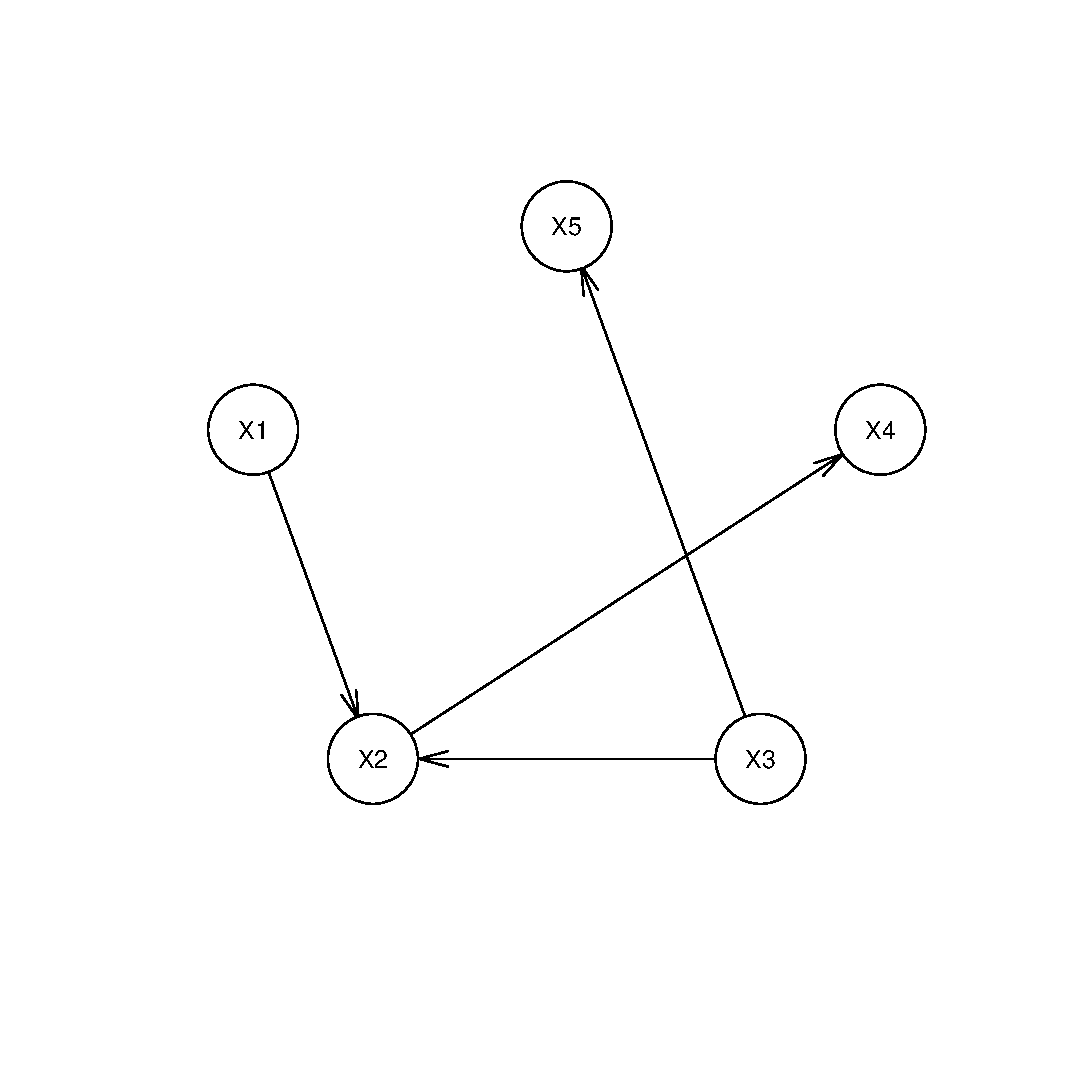
\includegraphics[width=5cm]{graphevermaexemple.eps} }
    \caption{Réseau} 
\end{figure} 
 
Si on voulait calculer une  probabilité jointe sans la propriété de factorisation, nous aurions besoin de connaître $2^{5}$ états, c'est à dire 32 états.


 Maintenant en tenant compte du théorème de la factorisation, nous n'avons plus besoin que des 10 données cité ci-dessous:  
$$\left\lbrace 
\begin{array}{lcl} 
  P(X_  1)  \\ 
P(X_2|X_1,X_3),\  P(X_2|\overline{X_1},X_3)  ,\ P(X_2|X_1,\overline{X_3}) ,\  P(X_2|\overline{X_1},\overline{X_3})\\ 
P(X_3)    \\
P(X_4|X_2) ,\  P(X_4|\overline{X_2})\\
P(X_5|X_3) ,\ P(X_5|\overline{X_3})\\
\end{array}\right.$$
Le produit de ces éléments nous donnera alors  la probabilité jointe. Cette propriété sera utilisé lorsqu'on parlera de génération de valeurs.

\subsection{Structures en séries, divergentes et convergentes}

Avant de passer au théorème fondamental qui va nous permettre d'interpréter les graphes,
nous devons définir 3 types de sous-structures particulières.

\subsubsection{Composantes en séries}

Supposons que nous ayons les événements en cascades  suivants:

-$X$ ="l'ensoleillement".

-$Y$="Prix du blé".

-$Z$="l'état de la récolte".

La structure va donc être mise  sous la forme: $X\longrightarrow Z \longrightarrow Y$.

Si nous supposons dans un premier temps  que la variable $Z$ est inconnue,
alors le fait que le temps soit ensoleillé aura une implication directe  sur le prix du blé et inversement.

$\Longrightarrow$ les variables  $X$ et $Y$ sont dépendantes.

Si maintenant nous fixons la variable $Z$,
alors l'état de la  récolte  aura une implication directe sur le prix du blé.
Dans ce cas de figure,
la connaissance de l'ensoleillement $X$ n'influencera plus le prix du blé.  

$\Longrightarrow$ les variables  $X$ et $Y$ deviennent indépendantes.


Nous dirons alors que \emph{le noeud $Z$ à l'interstice de deux variables $X$ et $Y$ bloque l'information pour une \definition{composante en série}}.

\subsubsection{Composante divergente}
Considérons  les événements suivants:

-$X$="La pelouse de mon jardin est humide".

-$Y$="La pelouse de mon voisin est humide".

-$Z$="Il a plu cette nuit".

La structure va donc être mise  sous la forme: $X\longleftarrow Z \longrightarrow Y$.

Si la pelouse de mon jardin est humide,
il y a de fortes chances de croire que la pelouse de mon voisin sera aussi humide.

Maintenant si je sais qu'il a plu cette nuit,
l'information concernant ma pelouse n'apportera plus aucun renseignement sur l'état de la pelouse de mon voisin:
elle sera automatiquement humide.


Nous dirons que \emph{le noeud $Z$ à l'interstice de deux variable $X$ et $Y$ bloque l'information pour une \definition{composante divergente}}

\subsubsection{Composante convergente ou V-structure}

Considérons les événements suivants:

-$X$="il y a eu un tremblement de terre ".

-$Z$="fonc\-tion\-ne\-ment de l'alarme de ma maison".

-$Y$="l'existence d'un cambriolage au sein de mon domicile".

La structure va donc être mise  sous la forme $X\longrightarrow Z \longleftarrow Y$.

A priori un lien de dépendance entre le tremblement de terre et le déroulement d'un cambriolage n'a pas lieu d'être.
Cependant si  l'alarme sonne,
la corrélation entre $X$ et $Y$ apparait.
En effet, si je sais qu'il y a eu un tremblement de terre,
automatiquement je diminue la plausibilité qu'il y ait eu un cambriolage.

Nous dirons que \emph{le noeud $Z$ à l'interstice de deux variables $X$ et $Y$ laisse passer l'information pour une \definition{composante convergente}}.

\textbf{Remarque:} 

Pour des causalité directes, il va de soi que l'information passe toujours.

L'union de ces trois composantes peut déjà  nous donner une idée sur le déplacement de l'information pour un réseau simple.
Nous utiliserons la notation \textit{on($Z$)} et \textit{off($Z$)} pour stipuler que la variable $Z$ est respectivement connue ou méconnue.


Considérons le cas suivant:


$$X_1\longrightarrow off(X_2) \longrightarrow on(X_3) \longrightarrow off(X_4) \longleftarrow X_5$$


La première sous-structure $X_1\longrightarrow off(X_2) \longrightarrow on(X_3)$ est en série, l'information passe alors  de $X_1$ à $X_3$ .
     
L'information partie de $X_1$ arrivée  en $X_3$ va pouvoir continuer son chemin jusque $X_5$ car la sous-structure  $X_3 \longrightarrow off(X_4) \longleftarrow X_5$  est convergente.  

En conclusion, l'information a pu se déplacer à travers la sous-structure: 

  $$X_1\longrightarrow off(X_2) \longrightarrow on(X_3) \longrightarrow off(X_4) \longleftarrow X_5$$  


Les réseaux définis précédemment sont  assez simple, le théorème nous permettant de traiter des réseaux du types complexes se nomme \emph{le théorème des D-séparations}.

\subsection{Théorème des D-séparation}

\begin{theorem}{Théorème}
Soit le graphe G($\aleph$,$\alpha$)  un Graphe orienté acyclique.

On note $<X|Z|Y>$  et on dit que X et Y sont D-séparés par Z si toutes  chaînes liants  X et Y vérifient au moins une des deux conditions suivantes:
\begin{itemize}
  \item Il existe  une composante convergente en un noeud $S \neq Z$ ou  $Z$ n'est pas une cause directe de $S$.
  \item Il existe  une composante divergente ou en série avec  $S=Z$.
\end{itemize}
\end{theorem}

Ce théorème nous montre la manière dont se déplace l'information dans n'importe quel réseau étant donné l'état $(on , off)$ du réseau.

En effet lorsque l'on a $<X|Z|Y>$,
la connaissance de l'interstice $Z$  bloque globalement l'information entre  $X$ et $Y$.
Dans le cas contraire,
le fait de ne pas avoir $<X|Z|Y>$ nous annonce que l'on aura au niveau de la chaîne liant $X$ et $Y$ une convergence V-structure en $Z$.

Cette dernière remarque est assez intéressante dans la mesure où elle nous interprète les V-structures comme étant des \textit{vannes laissant passer l'information à l'état $on$}
tandis que les structures en séries et divergentes seront interprétées comme des \textit{vannes laissant passer l'information à l'état off}.

Pour l'instant nous avons utilisé le théorème D-séparation pour analyser les déplacements d'informations étant donné la connaissance de l'état $on/off$ d'un réseau, cependant  nous n'avons à aucun moment parlé de probabilité.

Dans le prochain point,
un lien directe et important entre les D-séparations  et les indépendances conditionnelles lié à la probabilité sera établi.

\subsection{Théorème de Verma et Pearl}
\begin{theorem}{Théorème}

Si 2 variables $X$ et $Y$ sont D-séparées par une variable $Z$ alors $X$ et $Y$ sont indépendantes conditionnellement à $Z$:
 $$<X|Z|Y>\Longrightarrow X \ci Y|Z$$
\end{theorem}



\newpage
\subsection{Equivalence de réseaux bayésiens}

\subsubsection{Définition de l'équivalence de réseaux bayésien}

\definition{Deux réseaux bayésiens $B_1$ et $B_2$ sont dit équivalents} et noté $B_1\equiv B_2$  ssi ils représentent les mêmes indépendances conditionnelles.

Considérons les 2 réseaux bayésiens  en série suivants :
\[
\left\lbrace 
\begin{array}{lcl} 
B_1 \equiv A \longleftarrow B \longleftarrow C\\
B_2 \equiv A \longrightarrow B \longrightarrow C
\end{array}\right.
\]
Prouvons que ces deux réseaux sont bien équivalents.

\paragraph{Illustration}

En utilisant le théorème de factorisation de Verma : 
\[
P(A,B,C)_{B_{1}}=P(A / B).P(B/ C).P(C)
\]
$$P(A,B,C)_{B_{2}}=P(A).P(B / A).P(C / B)$$
Partons de la première relation et remplaçons à l'aide de la formule de bayes les probabilités  $P(A/B)$ et $P(B/C)$ en fonction respectivement des probabilités  $P(B/A)$ et $P(C/B)$ :

$$ P(A,B,C)_{B_{1}}=\frac{P(B/A).P(A)}{P(B)} .\frac{P(C/B).P(B)}{P(C)}.P(C)  \Longrightarrow  P(A,B,C)_{B_{1}}=P(A,B,C)_{B_{2}}$$

$\blacksquare$

Nous pouvons aussi  raisonner de la même façon pour une composante en divergence:
$$B_{3}\equiv A \longleftarrow B \longrightarrow C$$
qui sera alors équivalente à $B_{1}$ et $B_{2}$.

Seule la composante en V-structure 
$$B_{4}\equiv A \longrightarrow B \longleftarrow C$$
ne sera pas équivalente aux deux réseaux de départ.

\begin{align*}
P(A,B,C)_{B_{4}}&=P(B/A,C).P(A).P(C)\\
\end{align*}

Remarquons que l'illustration a été faite pour des réseaux Bayésiens simples.
Si maintenant nous avons un réseau Bayésien possédant  un grand nombre de noeuds,
l'analyse d'équivalence entre réseaux sera beaucoup moins triviale.
Il existe un théorème pouvant identifier des réseaux équivalents pour des structures complexes. 




\subsubsection{Théorème d'équivalence de réseaux}
\begin{theorem}{Théorème:}
  Deux réseaux bayésiens sont équivalents ssi ils ont le même squelette et le même ensemble de V-structures.
\end{theorem}

\textbf{Remarque:}


Le squelette  d'un graphe orienté acyclique est le graphe non-orienté obtenu en remplaçant les arcs par des arêtes.
Le squelette munis des V-structure est un graphe partiellement orienté;
on le nomme souvent \definition{graphe complété (CPDAG)} ou \definition{essentiel}.
Il va de soi alors qu'il existe une multitude de réseaux bayésien  équivalent associée à un graphe essentiel.

Si on veut obtenir un \textbf{CPDAG} à partir d'un graphe, il suffit de renverser des arcs correspondant aux  arrêtes du graphe essentiel  sans faire  apparaitre de V-structures.
Lorsqu'on réunit l'ensemble des réseaux équivalents,
on parle de \textbf{\textit{classe d'équivalence}}.


L'exemple qui suit  nous montre quelques réseaux équivalents déduits d'un graphe essentiels (CPDAG):

\begin{figure}[h]
\centering
\subfigure[CPDAG]{%
\fbox{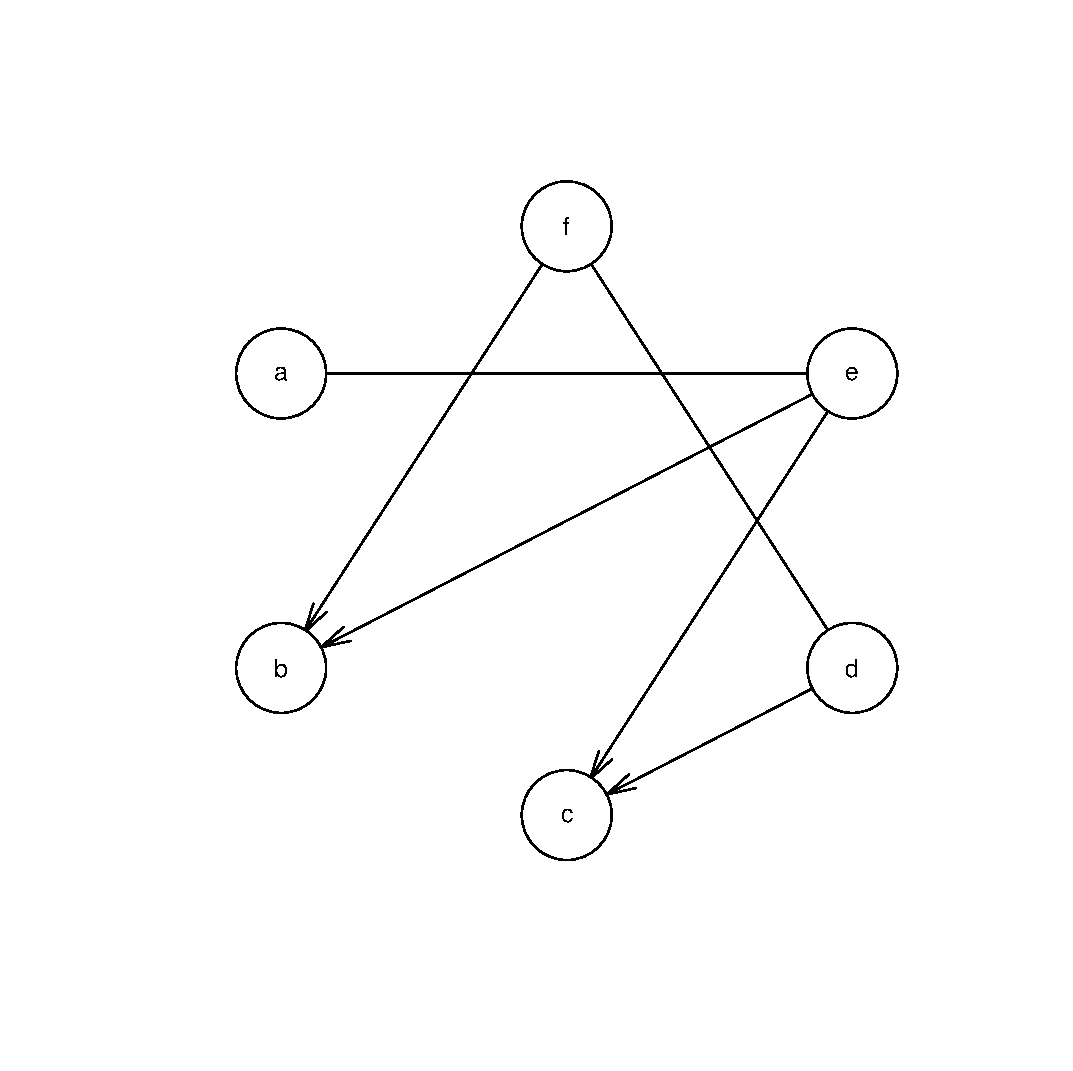
\includegraphics[width=0.4\textwidth]{IM_EQUIVAL_CPDAG.eps}}%
  }
$\quad$
\subfigure[Réseaux $B_1$]{

 \fbox{ 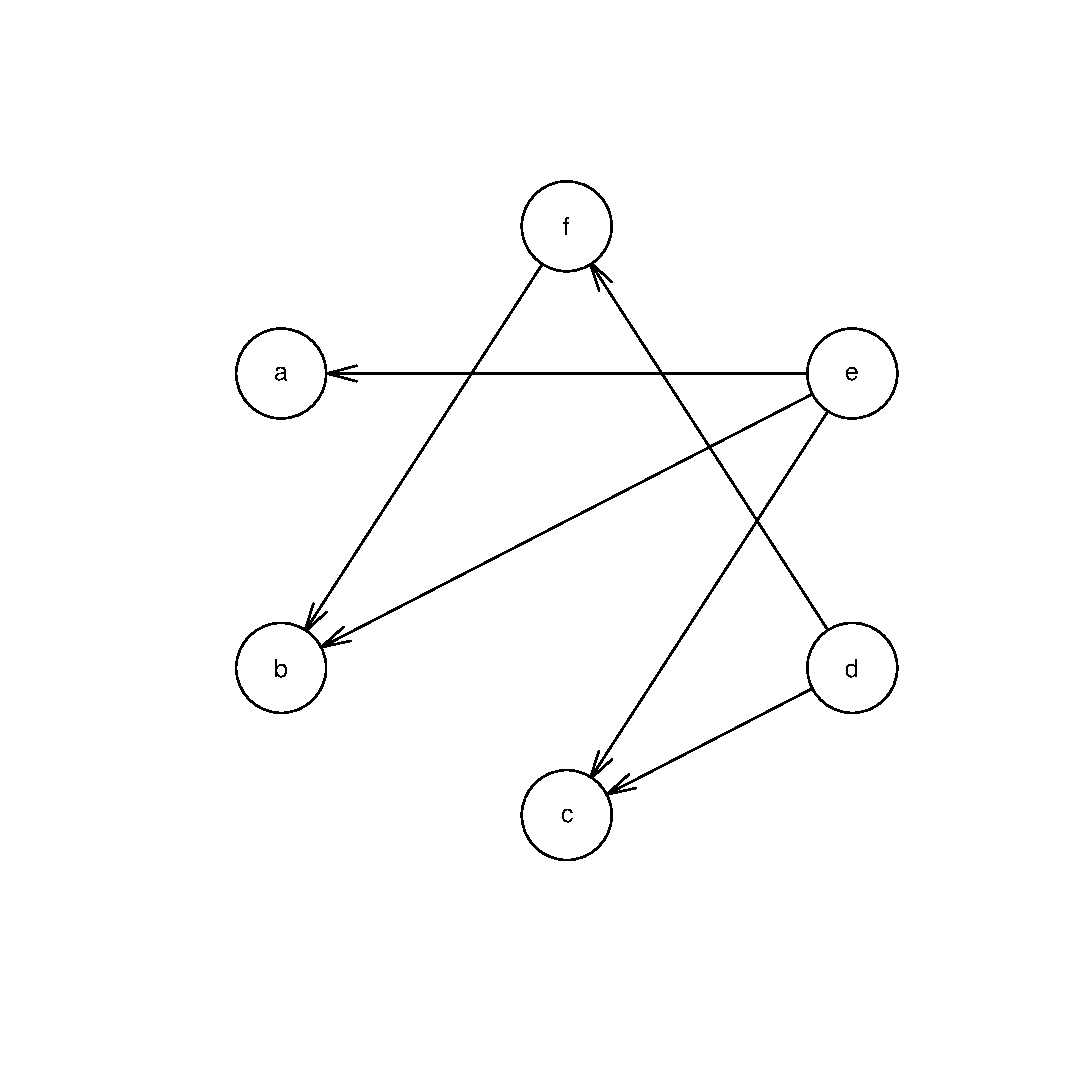
\includegraphics[width=0.4\textwidth]{IM_EQUIVAL_B_1.eps}}%
}   
\\
\subfigure[Réseaux $B_2$]{

\fbox{ 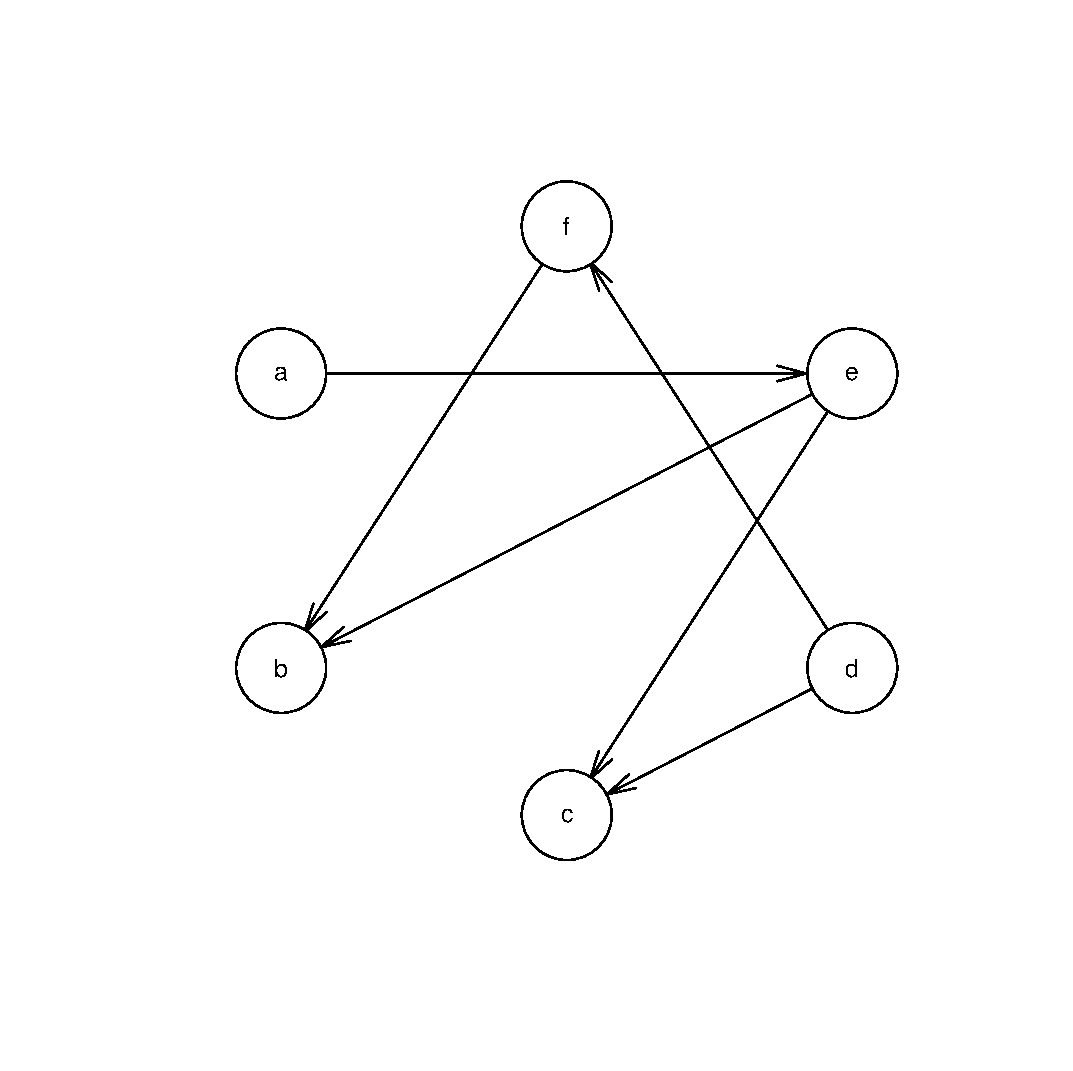
\includegraphics[width=0.4\textwidth]{IM_EQUIVAL_B_2.eps}}%
 }
$\quad$
\subfigure[Réseaux $B_3$]{
 \fbox{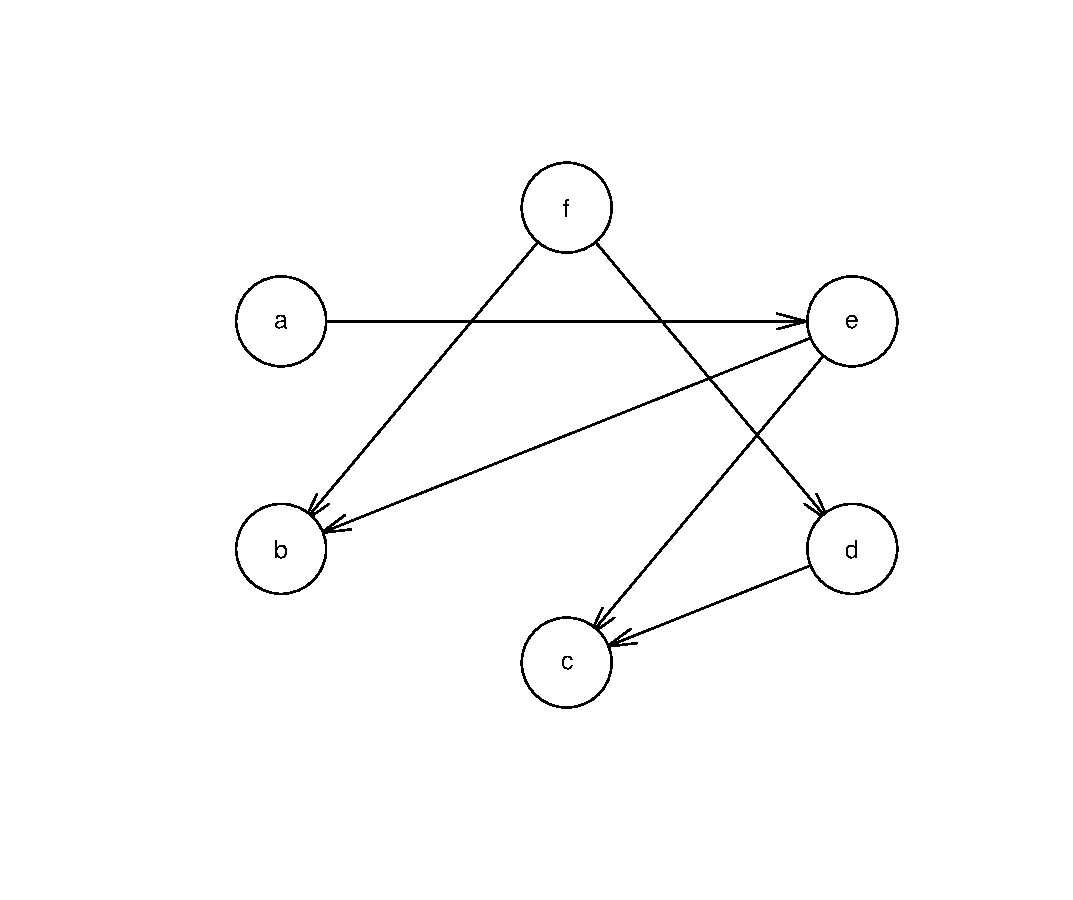
\includegraphics[width=0.4\textwidth]{IM_EQUIL_B_3.eps}}%
}
\end{figure}

Nous avons bien $B_1 \equiv B_2 \equiv B_3$ en faisant les inversion d'arcs $I$ suivantes:
$$CPDAG \Longrightarrow B_1 \Longrightarrow B_2=I_{(a,e)}(B_1) \Longrightarrow B_3=I_{(f,d)}(B_2).$$



\newpage

\section{Apprentissage de réseaux }

\subsection{Introduction}

L'espace des structures possibles est super-exponentiel pour le nombre de variables.
Le nombre $a_{k}$ de structures possibles pour $k$ noeuds (variables) est donné par la relation suivante :
$$a_{k}=\sum_{i=1}^{k}(-1)^{i+1} {k\choose i}2^{i(k-1)} a_{k-i}\approx k^{2^{O(k)}}$$
Nous avons donc un problème NP-complet.
Nous utiliserons alors des méthodes heuristiques d'apprentissages.

Nous allons dans cette section décrire les méthodes d'apprentissages de manière assez générale. 
Nous ne parlerons que des algorithmes d'apprentissages de jeux de données \emph{continues}.
Il existe deux familles d'algorithmes d'apprentissages de réseaux bayésiens:
\begin{enumerate}
  \item Algorithme basé sous-contraintes.
  \item Algorithme basé sur un score (une métrique).
\end{enumerate}

\subsection{Algorithme basé sous contraintes }

Les algorithmes basés sous-contraintes ont tous en commun les étapes suivantes:
\begin{itemize}
  \item Construire un graphe non-orienté  contenant les relations entre les variables. Ces relations sont déduites de tests d'indépendances.
  \item Détecter les V-structures en utilisant les test d'indépendances.
  \item Définir l'orientation des arcs restants en satisfaisant les contraintes de non-cycles.
\end{itemize}

\subsection{Algorithme basé sur un score}

Dans ce type d'algorithme, une construction itérative est évalué à l'aide d'une métrique mesurant la vraisemblance du réseaux par rapport à un jeux de donné.

Les deux métrique que nous allons utiliser dans l'apprentissage sont le suivantes:


\begin{itemize}
  \item la BGE-métrique que l'on peut retrouver dans l'article \textit{Learning Bayesian Network de David Heckerman et Dan Geiger}.

  \item La BIC-gaussienne qui est la \textit{bayésian  information criterion}. Elle est definis de manière général de la façon suivante :

$$ BIC(B,data)=max_{\Theta}\log P(B|data,\Theta)-\frac{d}{2}\log{n}$$

Où $d=\sum_{i=1}^{n} q_{i} (r_{i}-1) $ est la dimension de $B$.
La probabilité $P$ est une Gaussienne  multivariable.

\end{itemize}




\newpage

\section{Analyse de donnée}

\subsection{Introduction}
Dans ce point nous montrerons les trois outils statistiques qui vont être utilisé dans  notre analyse de données.
La validation se fera par des  test d'hypothèses sur les corrélations qui seront de deux types:

\begin{enumerate}
  \item Les corrélations globales du type $\rho_{XY}$ liées  au dépendances  directes dans la représentation bayésienne.

Il est à noter que la corrélation est parfaitement symétrique $\rho_{XY}=\rho_{YX}$ ,ceci impliquera que l'orientation d'un arc entre deux noeuds adjacents n'aura pas d'influence dans nos interprétations.    

Formule de $\rho_{XY}$:
\begin{equation}
\rho_{XY}=\frac{\sum_{i=1}^{n}(X_i-\overline{X}).(Y_i-\overline{Y})}{\sqrt{\sum_{i=1}^{n}(X_i-\overline{X})^{2}} .\sqrt{\sum_{i=1}^{n}(Y_i-\overline{Y})^{2}}}
\end{equation}
Les outils d'analyses statistiques utilisés seront les test d'indépendances du types Students ainsi que l'analyse en composantes principales.



\item Les corrélations partielles $\rho_{XY|Z}$, liées aux dépendances indirectes, seront interprété par l'utilisation du théorème des D-séparations et la validation se fera par test d'hypothèses de  type Students.

Formule de $\rho_{XY|Z}$ pour une seule variable $Z$:
\begin{equation}
\rho_{XY|Z}=\frac{\rho_{XY}-\rho_{XZ}\rho_{ZY}}{\sqrt{1-\rho_{XZ}^{2}\sqrt{1-\rho_{ZY}^{2}}}}
\end{equation}

\end{enumerate}







\newpage
\subsection{Analyse en composantes principales (ACP)}
Considérons  un système de $p$ variables $X_{1...p}$ où l'on veut étudier la variabilité.

L'objectif de l' ACP sera d'utiliser un nombre $q$ de variables inférieurs à $p$ nous permettant d'étudier au maximum la variabilité du système.
Pour cela nous allons chercher un nouveaux système d'axes maximisant la variance $\sigma^{2}$. 

Intérêts la méthode:

\begin{itemize}
  \item Réduire le nombre de variables descriptives.
  \item Obtenir une visualisation inter-variable en  2D(cercle) ou 3D(sphère).

\end{itemize}




Lorsque les critères suivent des échelles différentes, on utilise \textit{une analyse en composantes principales normées}  en remplaçant les éléments $a_{i,j}$ par $a_{i,j}'$:
$$a_{i,j}'=\frac{a_{ij}-\overline{a_{j}}}{\sqrt{k} .s_{j}}$$

où
$$s_{j}^{2}=\frac{1}{k}\sum_{i=1}^{k}(a_{ij}-\overline{a_{j}})^{2}$$

est la variance de $j^{e}$ caractère. 


Dans le cas d'une ACP 2D, le cercle unitaire dans lequel est projeté le nuage de points se nomme: \textit{le cercle des corrélations}.

On peut alors démontrer que :

$$||X_{i},X_{j})||=\sqrt{2(1-\rho_{X_{i}X_{j}})}$$

où $X_{i}$ et $X_{j}$ sont les points représenté dans le cercle des corrélations.



L'interprétation du cercle de corrélation est alors la suivante:

\begin{itemize}
  \item La distance entre 2 points est toujours comprise entre 0 et 2.
  \item Si elle est proche de 0, cela signifie que les 2 caractères sont fortement corrélés positivement.
   \item Si elle est proche de $\sqrt{2}$, cela signifie que les 2 caractères sont peu corrélés.
   \item Si elle est proche de 2, cela signifie que les 2 caractères sont fortement corrélés négativement.

\end{itemize}

Nous utiliserons dans nos analyses statistiques la quantité d'information $\delta$ comme étant le pourcentage de variance expliqué par une représentation 2D ou 3D.
\[
\left\lbrace 
\begin{array}{lcl}
\delta=\frac{\lambda_{1}+\lambda_{2}}{\sum_{i=1}^{p}\lambda_{i}} \ \ ACP \ 2D\\ \\

\delta=\frac{\lambda_{1}+\lambda_{2}+\lambda_{3}}{\sum_{i=1}^{p}\lambda_{i}} \ \ ACP \ 3D

\end{array}\right.
\]
où les $\{\lambda_{i}\}$ correspondent aux valeurs propres de la matrice des corrélations. Nous estimerons que $\delta$ est raisonnable pour des valeurs $\approx 90\%$ 

\newpage
\subsection{Test statistiques Student pour la corrélation}

Le test d'hypothèse du coefficient de corrélation $\rho_{XY}$ et $\rho_{XY|Z}$ est fait de manière classique à l'aide d'un test de Student.{\\}
Dans le cas où nous sommes dans  l'hypothèse nulle $H_{0}$, nous avons l'absence de liaison entre $X$ et $Y$. 

Sous l'hypothèse nulle, le rapport de l'estimateur du coefficient de corrélation $r$ sur son écart-type suit une loi de Student à $(n-2)$ de degré de liberté:

$$\frac{r}{s_{r}} \longrightarrow t_{(n-2)ddl}\text{  avec  } s_{r}=\sqrt{\frac{(1-r^{2})}{(n-2)}}$$

Le test consiste à comparer le ratio à une valeur seuil $t_{\alpha}$ sur la table de la lois de Student à $(n-2)$ degré de liberté.

\fbox{\textit{Nous choisirons dans notre cas une hypothèse nulle à rejetter pour une P-value $\le$ 0.1.}}

\subsection{Diagramme en boîte}

Ce diagramme nous permettra de  visualiser la position des médianes, des quartiles, des minimum et des maximum entre les jeux de données réalistes et artificiels.

Le diagramme se présente comme suite:
\begin{figure}[H] 
    \center
    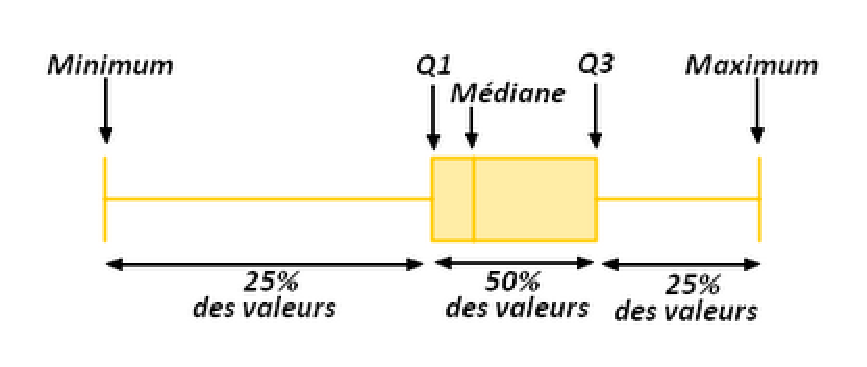
\includegraphics[width=10cm]{boiteanmoustache.eps} 
    \caption{Diagramme en boîte} 
\end{figure}
où
$Q_{1}$ et $Q_{2}$ correspondent respectivement aux premiers et troisièmes quartiles.









\newpage

\section{Apprentissage des réseaux bayésiens au problèmes multicritères}

\subsection{Introduction}

Dans cette section , nous allons apprendre un réseaux bayésiens à partir d'un jeux de données où les alternatives sont des voiture en fonction de certains critères tel que le prix , l'accélération etc.


La même analyse sera établit pour d'autres jeux de données.( cf. annexe \ref{apprentissage_usine} et annexe \ref{apprentissage_guitare}). 
 
 L'étude statistique se fera sur le jeux départ et celui obtenu après la génération de \textbf{ 1000 valeurs} inférés sur base du réseaux appris.


Les deux types d'apprentissage associés aux deux métriques (BGE-métrique et BIC-métrique) seront appliqués aux jeux de données et nous procéderons alors à une validation d'une métrique en vertu de l'autre.

La validation de la métrique sera faite en fonction de la cohérence qu'il existera entre le réseaux appris et le principe des D-séparations.

 Nous ajouterons  ensuite deux types de bruitages brut sur les jeux de données:

\begin{itemize}
  \item Un léger bruitage permettant de tester la robustesse du réseaux appris. Ce type de bruitage sera uniquement  effectué sur le jeux de données concernant l'achat d'une voiture. 

  \item Un grand bruitage permettant d'atténuer les corrélations en agissant directement sur le jeux de données.

Nous verrons que cette méthode n'est pas très efficace dans l'ajustement des corrélations.

Vous trouverez en annexe \ref{programme} , les deux programmes en $R$ qui ont été utilisés.   

\end{itemize}



Une dernière section vérifiera que le jeux de données générés de 1000 valeurs nous donne bien des individus proches de ceux provenant  du jeux de données initial. Pour étudier la proximité des individus générés par rapport aux individus initiaux, nous utiliserons une ACP ainsi qu'un diagramme en boîte.

\newpage
\subsection{Problème: Achat d'une voiture}
\subsubsection{Tableaux de données}
Un décideur est amené à choisir une voiture suivants les critères décrits ci-dessous: 

\begin{figure}[H] 
    \center
    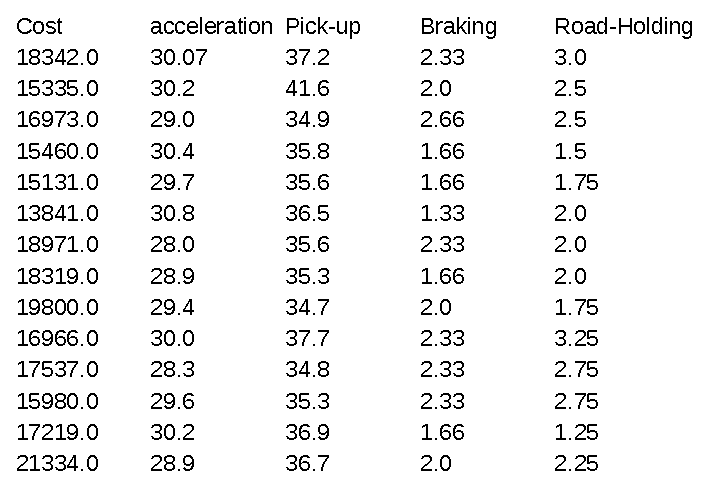
\includegraphics[width=7cm]{Thierry.eps} 
    \label{figdepart}
\end{figure} 

\subsubsection{Application de la BIC-métrique}

En appliquant l'algorithme d'apprentissage de type BIC-métrique, nous obtenons le réseau suivant:

\begin{figure}[H] 
    \center
    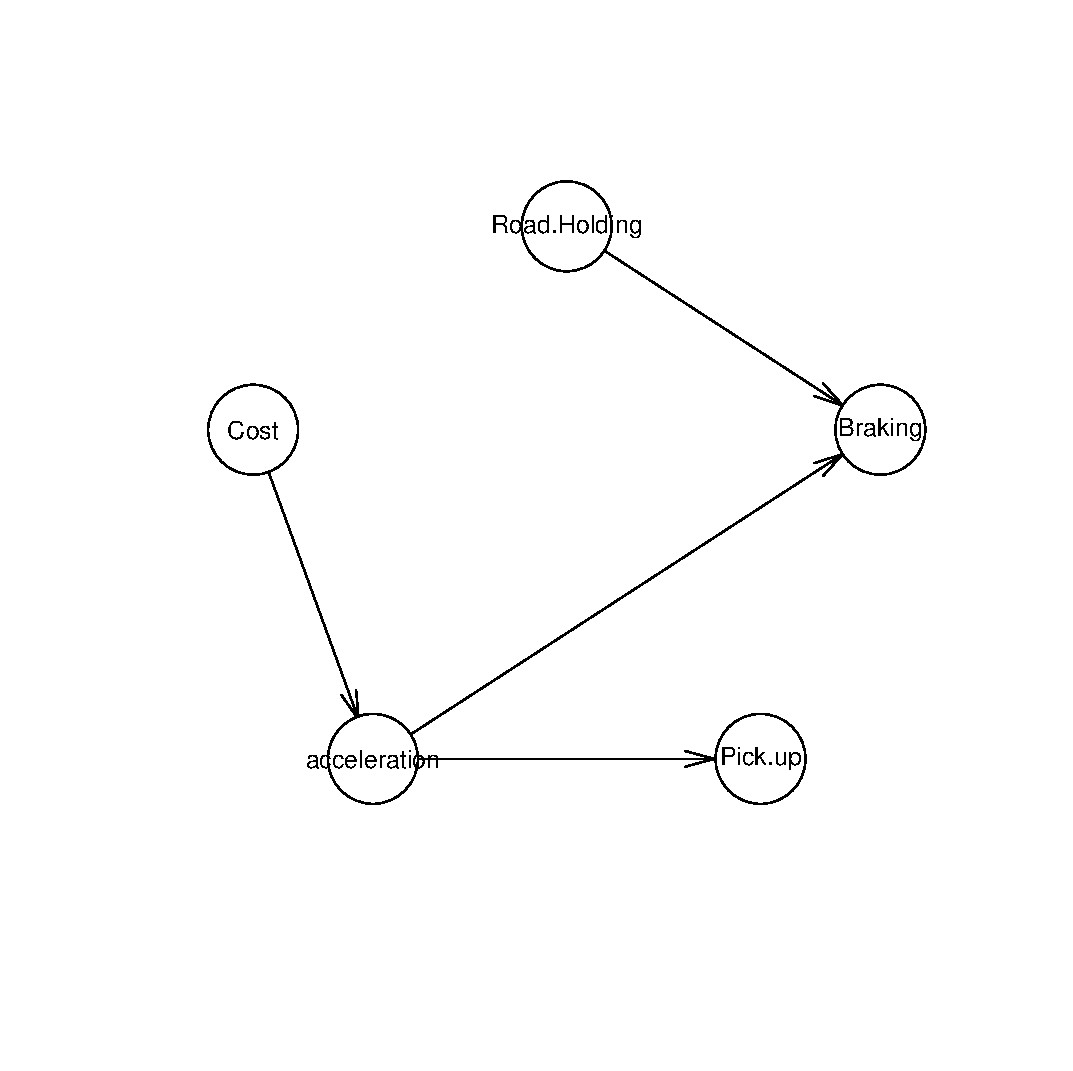
\includegraphics[width=5cm]{THIERRY_GRAPHE.eps} 
    \caption{Réseau obtenu après l'application de la BIC-métrique} 
	\label{bicmetric}
\end{figure}

Nous allons maintenant vérifier que le réseau précédent répond correctement de manière statistique au principe des D-séparations.
Nous représentons dans les tableaux Fig.\ref{tab1_14} et Fig.\ref{tab1_1000} qui suivent les différentes corrélations ainsi que la P-value associée aux test d'hypothèses de type Student. 
Les évaluations sont faites pour le jeux des 14 alternatives de départ  et pour celui obtenu après la génération de 1000 valeurs.

\begin{figure}[H]
\begin{center}
\begin{tabular}{|l|c|r|}
  \hline
  Relation & Corrélation & P-value \\
  \hline
   Road.Holding $\cap$  acceleration&$-0.1266$& =0.6662 \\
   Road.Holding $\cap$  acceleration $|$Braking &$0.3871$& $0.1913$  \\
\hline \hline \\
Cost $\cap$ Braking &0.3584&$0.2083$\\
Cost $\cap$ Braking$|$accelaration &0.0447&0.8848\\
\hline \hline 
Cost $\cap$ Road.Holding $|$ Braking&-0.2942&$ 0.3292$\\
Cost $\cap$ Road.Holding &0.0522&0.8592\\
Cost$\cap$Road.Holding$|$acceleration&0.0356&0.908\\
Cost $\cap$ Road.Holding $|$ acceleration $\cup$ Braking&-0.1033&0.7493\\
\hline
\end{tabular}
\end{center}
\caption{Test statistiques pour le jeux de données de 14 alternatives }
\label{tab1_14}
\end{figure}





\begin{figure}[H]
\begin{center}
\begin{tabular}{|l|c|r|}
  \hline
  Relation & Corrélation & P-value \\
  \hline
   Road.Holding $\cap$  acceleration&$-2.10^{-4}$& =0.9962  \\
   Road.Holding $\cap$  acceleration $|$Braking &$0.4607$& $<2,2.10^{-16}$  \\
\hline \hline \\
Cost $\cap$ Braking &0.2741&$<2.2.10^{-16}$\\
Cost $\cap$ Braking$|$accelaration &-0.0299&0.3446\\
\hline \hline 
Cost $\cap$ Road.Holding $|$ Braking&-0.288&$ < 2,2.10^{-16}$\\
Cost $\cap$ Road.Holding &-0.0213&0.5005\\
Cost$\cap$Road.Holding$|$acceleration&-0.0282&0.3739\\
Cost $\cap$ Road.Holding $|$ acceleration $\cup$ Braking&-0.0085&0.7874\\
\hline
\end{tabular}
\end{center}
\caption{Test statistiques pour le jeux de données de 1000 valeurs }
\label{tab1_1000}
\end{figure}

\textbf{Commentaires:}
\begin{itemize}
  \item \underline{Pour les variables  $\{Road.Holding,Braking,acceleration\}$}:{\\}


Les deux variables $ Road.Holding$ et $acceleration$ sont liées par une V-structure, ceci a pour conséquence que la méconnaissance de la variable $Braking$ bloque l'information:

 $$Road.Holding \not\ci  acceleration.$$

 La connaissance de $Braking$ va donc  laisser circuler l'information:

 $$ Road.Holding  \ci  acceleration  | Braking.$$


\item\underline{ Pour les variables $\{Cost,acceleration,Braking\}$}:{\\}


Les variables $Cost$ et $Braking$ sont liées par une structure en série, ce qui implique que les variables  sont dépendantes sans conditionnement.

La variable $acceleration$ bloque alors l'information de $Cost$ à $Braking$.

\item\underline{ Pour les variables $\{Cost,acceleration,braking,Road.Holding\}$}{\\}


La chaîne liant $Cost$ et $Road.holding$ passe par les deux noeuds $accelleration$ et $ Braking$.

Nous avons donc une structure série suivi d'une V-structure.
En conditionnant  par $Braking$ nous accentuons la dépendance, en effet  nous sommes dans une configuration de méconnaissance de l'interstice de la structure en série  et de la connaissance de la V-structure.

Progressivement en faisant l'opération $off(Braking)$ et $on(acceleration$), nous diminuons la circulation d'information et par conséquent la corrélation.
\end{itemize}

\textbf{En résumé}:

Les résultats obtenus du point de vue statistique sont cohérents avec le principe des D-séparations.

Lorsqu'on génère 1000 valeurs, la P-value vient accentuer la propriété des D-séparations.


























\subsubsection{Application de la BGE-métrique}
Dans cette section nous appliquerons la BGE-métrique et nous comparons le réseau appris par cette métrique avec le réseau obtenu au point précédent.

En appliquant le BGE-métrique à notre jeux de données des 14 valeurs:
 
\begin{figure}[H] 
    \center
    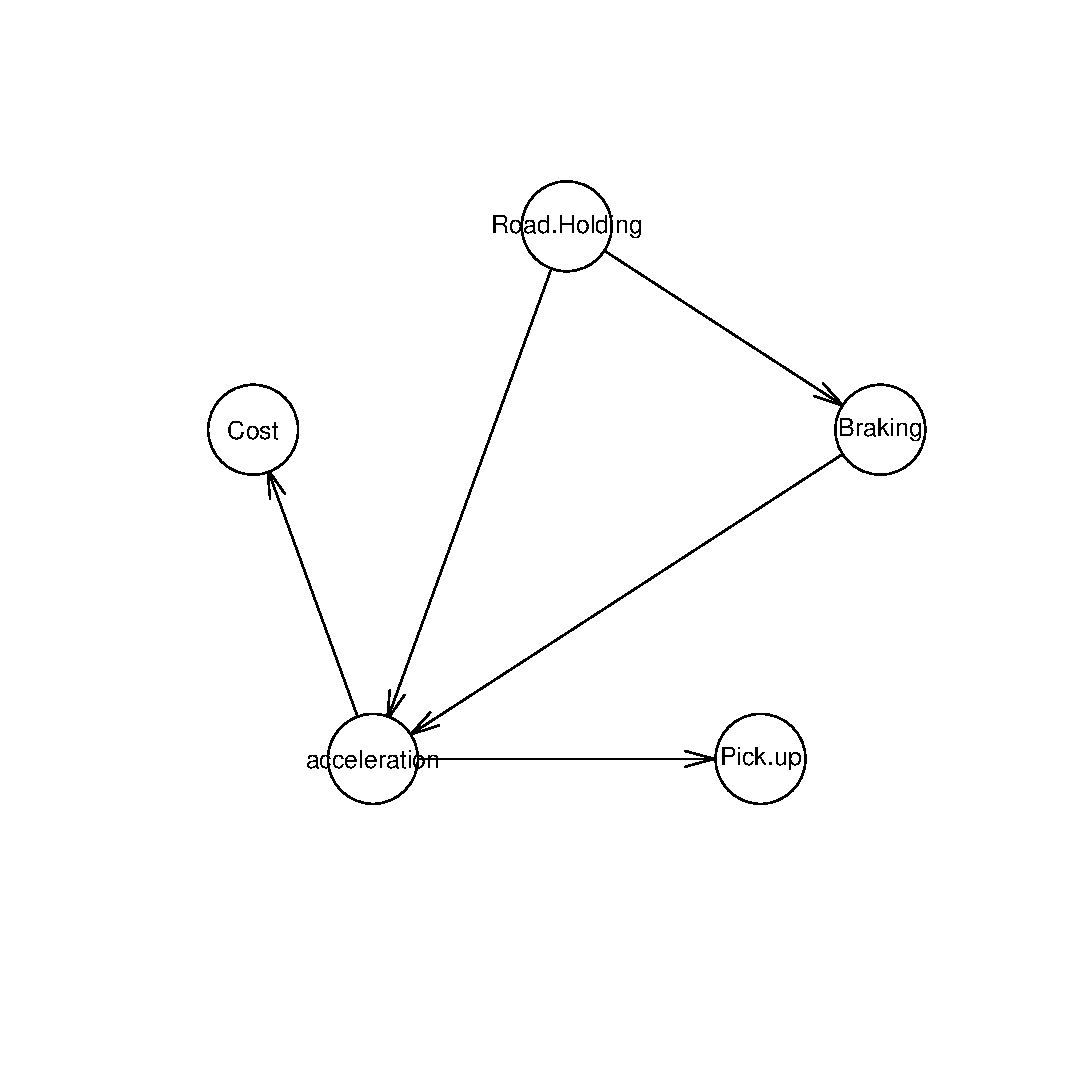
\includegraphics[width=5cm]{THIERRY_IMAGE_BGE.eps} 
    \caption{Application de la BGE-métrique au jeux de données} 
\end{figure} 

Nous remarquons que nous n'avons pas la même structure bayésienne qu'au point précédent.

 Le réseaux le plus adaptée au jeux de valeurs est celui décrit par la BIC-métrique.

En effet si nous observons  le triplet $(acceleration,Braking,Road.Holding)$, celui-ci se comporte comme une  V-structure.
Cette observation est décrite dans le tableaux Fig.\ref{fig2_vstruct}:

\begin{figure}[H]
\begin{center}
\begin{tabular}{|l|c|r|}
  \hline
  Relation & Corrélation & P-value \\
  \hline
acceleration $\cap$ Road.Holding & $-0.1266$&=0.662 \\
acceleration $\cap$ Road.Holding $|$ Braking& 0.3871&$=0.1913$.\\ 
\hline
\end{tabular}
\end{center}
\caption{Test statistiques pour les 14 alternatives }
\label{fig2_vstruct}
\end{figure}




\subsubsection{Normalisation, ACP 2D et tableaux des corrélations}

En sorti de la fonction du grand bruitage , on obtient un jeux de donnée normalisé et c'est pour cela que nous travaillerons avec le jeux de départ normalisé afin faciliter la comparaison.



Nous utiliserons une ACP 2D et la matrice des corrélations comme outils de base pour analyser si le jeux est assez bruité.

Nous ajouterons du bruit si nécessaire sur les jeux de donné  de tel sorte à obtenir des corrélations atténuées. 



Pour le jeux de départ, on retrouve le tableaux de données normalisés Fig.\ref{tab_data1}, la matrice de corrélation Fig. \ref{matcorr1} ainsi que l' ACP  2D Fig.\ref{acp1}.

\begin{figure}[H]
\begin{tabular}{llllll}
  \hline
Altérnatives&  Cost & acccélération & Pick.up&Braking&Road.Holding \\
  \hline
1& 0.07604225 &  0.07272595      & 0.07386067    & 0.08239038        &0.096\\
2&0.06357583   &0.07304037        &0.08259688     &0.07072136        &0.080\\
 3&0.07036665   &0.07013810       &0.06929402     &0.09405941        &0.080\\
 4&0.06409406   &0.07352408       &0.07108097     &0.05869873        &0.048\\
 5&0.06273009   &0.07183109       &0.07068387     &0.05869873        &0.056\\
6&0.05738201   &0.07449150       &0.07247082     &0.04702970        &0.064\\
 7&0.07864996   &0.06771954      &0.07068387     &0.08239038        &0.064\\
8& 0.07594690   &0.06989624      &0.07008822     &0.05869873        &0.064\\
9&0.08208683   &0.07110552      &0.06889692      &0.07072136        &0.056\\
10& 0.07033763   &0.07255665     &0.07485342      &0.08239038        &0.104\\
 11&0.07270489   &0.06844511     &0.06909547      &0.08239038        &0.088\\
12&0.06624988   &0.07158923      &0.07008822      &0.08239038        &0.088\\
13&0.07138652   &0.07304037     &0.07326502      &0.05869873        &0.040\\
14&0.08844649   &0.06989624     &0.06304164      &0.07072136        &0.072\\

\hline

\end{tabular}
\caption{Jeux de données normalisés}
\label{tab_data1}
\end{figure}



\begin{figure}[H]
\begin{tabular}{llllll}
  \hline
                &  Cost & acccélération & Pick.up&Braking&Road.Holding \\
  \hline
Cost          &1.00000000  & -0.6293580& -0.55805385 & 0.35838862 &  0.05223773\\
acceleration& -0.62935802 &   1.0000000 & 0.52595617 &-0.52243621 & -0.12663539\\
Pick.up      &-0.55805385   & 0.5259562  &1.00000000 &-0.06742284   &0.18436969\\
Braking       &0.35838862   &-0.5224362 &-0.06742284  &1.00000000   &0.69604522\\
Road.Holding & 0.05223773  & -0.1266354 & 0.18436969 & 0.69604522 &  1.00000000\\

\hline

\end{tabular}
\caption{Tableaux des corrélations}
\label{matcorr1}
\end{figure}


\begin{figure}[H] 
    \center 
    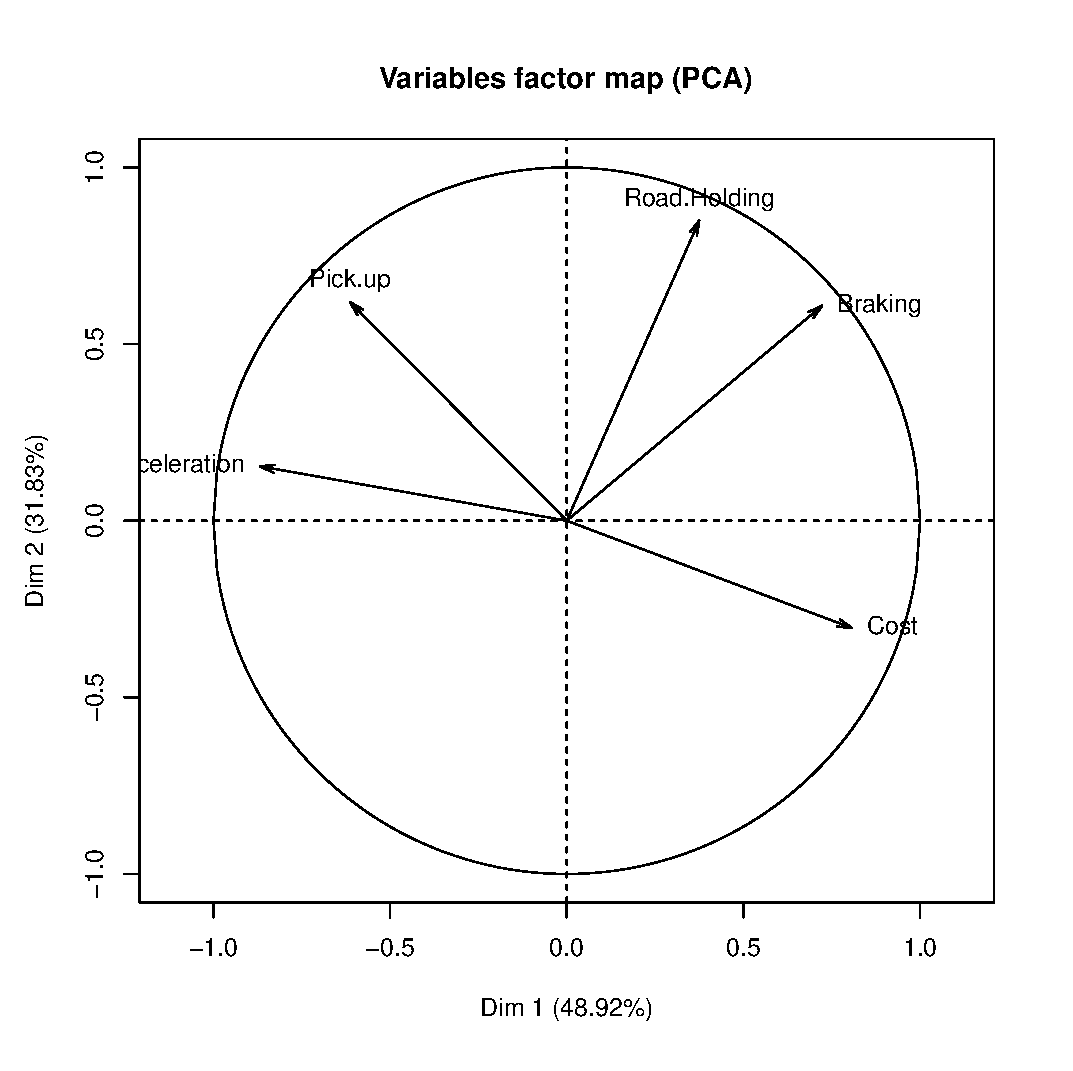
\includegraphics[width=8cm]{PCA_THIERRY.eps} 
    \caption{Représentation en  ACP 2D} 
\label{acp1}
\end{figure} 

\subsubsection{Test de robustesse par faible bruitage}

Dans cette section  nous observons la petite  variation à ajouter sur le critère $Cost$ pour que le réseau se modifie. Le jeux de données de départ Fig.\ref{figdepart} devient  :
\begin{figure}[H]
\begin{tabular}{llllll}
  \hline
Altérnatives&  Cost & acccélération & Pick.up&Braking&Road.Holding \\
  \hline
1 & 18344.75        &30.07    &37.2    &2.33         &3.00\\
2  &15337.30        &30.20    &41.6    &2.00         &2.50\\
3  &16975.55        &29.00    &34.9    &2.66         &2.50\\
4  &15462.32        &30.40    &35.8    &1.66         &1.50\\
5  &15133.27        &29.70    &35.6    &1.66         &1.75\\
6  &13843.08        &30.80    &36.5    &1.33         &2.00\\
7  &18973.85        &28.00    &35.6    &2.33         &2.00\\
8  &18321.75        &28.90    &35.3    &1.66         &2.00\\
9  &19802.97        &29.40    &34.7    &2.00         &1.75\\
10 &16968.55        &30.00    &37.7    &2.33         &3.25\\
11 &17539.63        &28.30    &34.8    &2.33         &2.75\\
12 &15982.40        &29.60    &35.3    &2.33         &2.75\\
13 &17221.58        &30.20    &36.9    &1.66         &1.25\\
14 &21337.20        &28.90    &36.7    &2.00         &2.25\\

\hline

\end{tabular}
\caption{Jeux de données obtenu à partir du faible bruitage}
\end{figure}

\begin{figure}[H] 
    \center 
   \fbox{ 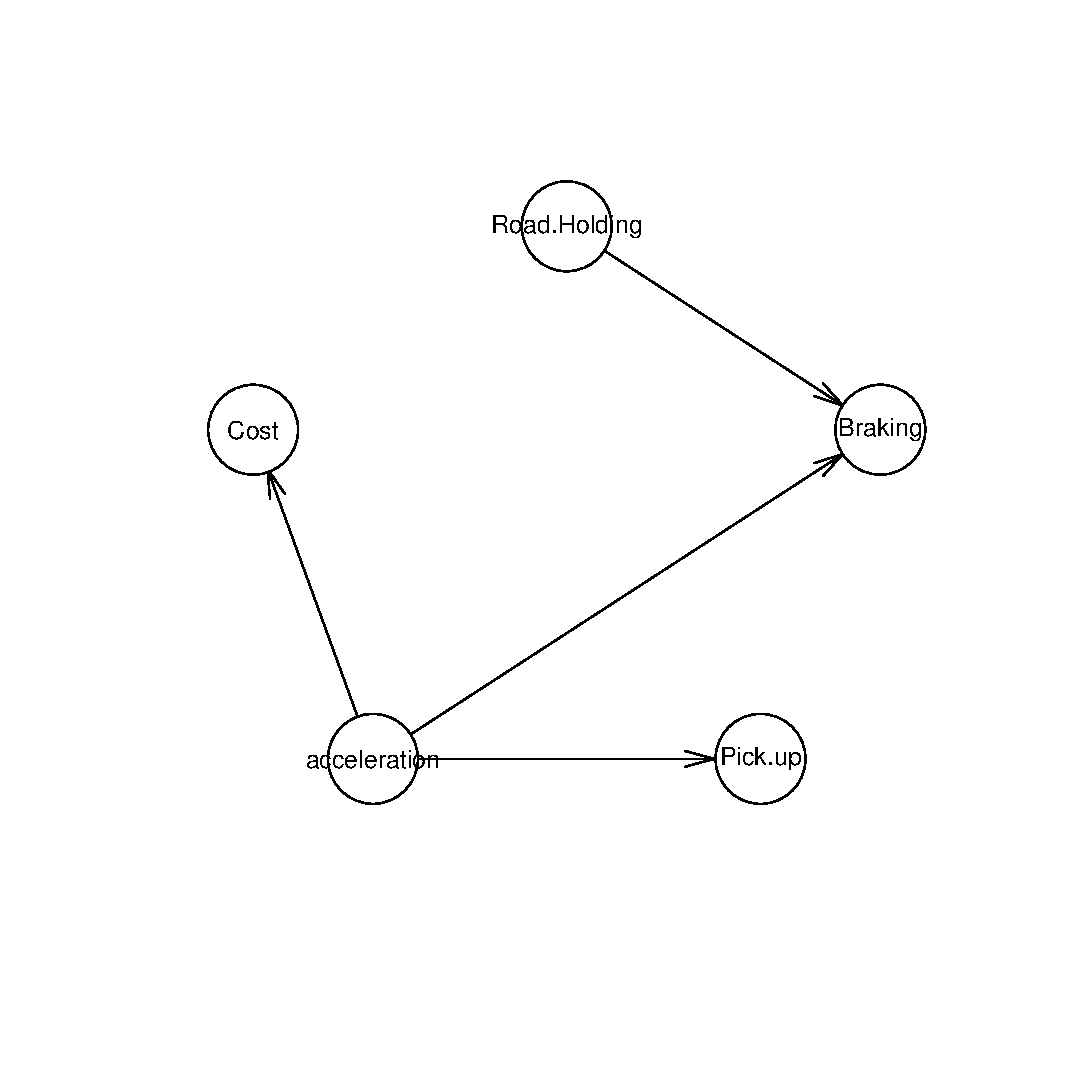
\includegraphics[width=5cm]{GRAPHE_THIERRY_BRUIT_FAIBLE.eps} }
    \caption{Réseau associé au jeux faiblement bruité} 
\end{figure} 

\textbf{Commentaire}:

Si nous comparons le tableaux précédent  avec le tableaux de données initial non-normalisé, nous remarquons que la petite variation effectuée sur le critère $Cost$ ne change pas  notre matrice de corrélation. Par contre l'arc liant les deux noeuds $Cost$ et $Road.holding$ a été inversé.


\textit{Cet ajout de faible bruitage caractérise un réseaux bayésien appris comme étant  fort sensible aux modifications effectuées sur le jeux de données. }



\subsubsection{Atténuation de la corrélation par grand bruitage du jeux de données}

 L'objectif de cette méthode est d'atténuer les corrélations trop importantes.

 Cette méthode reçoit en entrée : Le jeux de données , le critère primaire à bruiter ,le deuxième critère par rapport au quelle le premier critère sera décorrélé , le pourcentage décorrélation voulu, deux bornes de variation d'ajout sur le jeux de données initiales.

La méthode nous donne en sortie  un jeux de données \textit{ normalisé}  et corrélé de façon désiré.

Dans notre exemple, nous avons une corrélation entre la variable  $Cost$ et la variable $acceleration$ qui est trop importante ( =-0.6293580).

Nous allons donc décorréler les variables  en appliquant la méthode des grand bruitages sur le premier critère $Cost$.

Dans ce cas, nous dirons que $Cost$ est bruité par rapport à $acceleration$ en utilisant la notation: \textbf{ Cost/acceleration}.

En appliquant le programme d'ajout de grand bruitage  définis en annexe \ref{programme} on obtient le tableaux de données Fig.\ref{tabdata2} et la matrice des corrélations Fig\ref{matcorr2}  :

\begin{figure}[H]
\begin{tabular}{llllll}
  \hline
Altérnatives&  Cost & acccélération & Pick.up&Braking&Road.Holding \\
  \hline
1 & 0.07492529   &0.07272595   & 0.07386067   &0.08239038        &0.096\\
2  &0.09082277   &0.07304037    & 0.08259688   &0.07072136        &0.080\\
3  &0.06263684   &0.07013810     &0.06929402   &0.09405941        &0.080\\
4  &0.04631052   &0.07352408      &0.07108097   &0.05869873        &0.048\\
5  &0.05646680   &0.07183109      &0.07068387   &0.05869873        &0.056\\
6  &0.04157444   &0.07449150     &0.07247082   &0.04702970        &0.064\\
7  &0.09786636   &0.06771954     &0.07068387   &0.08239038        &0.064\\
8  &0.05812170   &0.06989624     &0.07008822   &0.05869873        &0.064\\
9  &0.11016151   &0.07110552    &0.06889692   &0.07072136        &0.056\\
10 &0.10455715   &0.07255665   &0.07485342   &0.08239038        &0.104\\
11 &0.04720490   &0.06844511    &0.06909547   &0.08239038        &0.088\\
12 &0.07049429   &0.07158923    &0.07008822   &0.08239038        &0.088\\
13 &0.06125340   &0.07304037   &0.07326502   &0.05869873        &0.040\\
14 &0.07760403   &0.06989624    &0.06304164   &0.07072136        &0.072\\

\hline

\end{tabular}
\caption{Jeux de données normalisé obtenu avec les paramètres d'entrées:(data,1,2,0.4,100,200)}
\label{tabdata2}
\end{figure}

\begin{figure}[H]
\begin{tabular}{llllll}
  \hline
                &  Cost & acccélération & Pick.up&Braking&Road.Holding \\
  \hline
Cost      &    1.0000000  & -0.1910163 & 0.18878857 & 0.43932168  &  0.2794929\\
acceleration& -0.1910163  &  1.0000000 & 0.52595617& -0.52243621 &  -0.1266354\\
Pick.up       &0.1887886    &0.5259562  &1.00000000 &-0.06742284    &0.1843697\\
Braking       &0.4393217   &-0.5224362 &-0.06742284  &1.00000000    &0.6960452\\
Road.Holding & 0.2794929  & -0.1266354 & 0.18436969 & 0.69604522  &  1.0000000\\

\hline

\end{tabular}
\caption{Tableaux des corrélations du nouveaux jeux bruité}
\label{matcorr2}
\end{figure}

\underline{\textbf{Commentaire}} :


Nous avons ajouté du bruit sur le critère n°1 $Cost$ en demandant une atténuation minimum de 40 \% sur la corrélation $\rho_{Cost,acceleration}$ . 

La nouvelle matrice de corrélation a été modifié sur la première ligne et la première colonne, les autres corrélations n'ont pas été modifiées.

On obtient après l'ajout de bruit  l' ACP 2D Fig.\ref{acpbruit}:

\begin{figure}[H] 
    \center 
    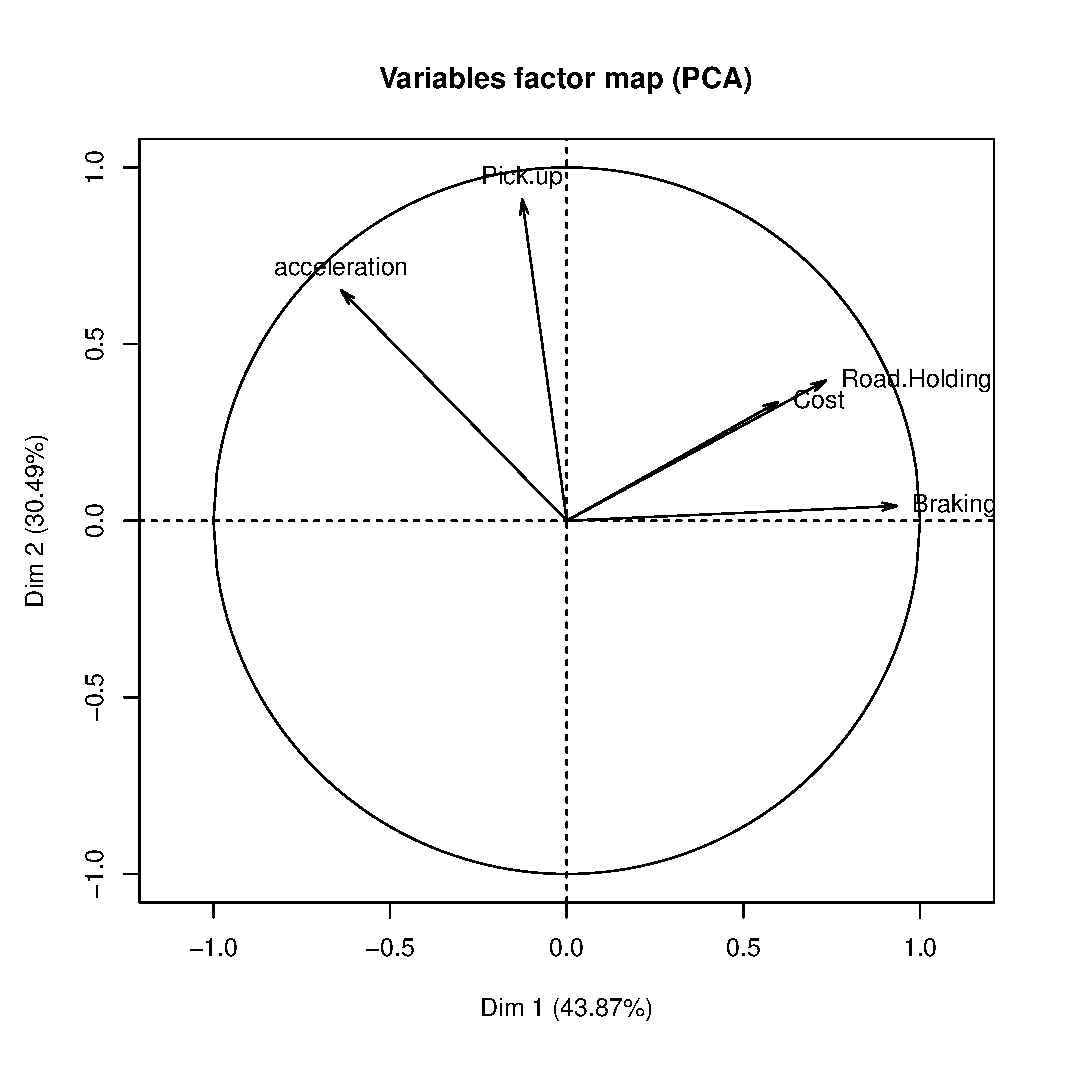
\includegraphics[width=7cm]{GRAP_THIERRY_FORT_BRUIT.eps} 
    \caption{Représentation d'une ACP 2D du nouveaux jeux de données bruité} 
\label{acpbruit}
\end{figure} 

 L' ACP 2D nous montre que nous avons encore une trop grande corrélation entre les variables  $Cost$ et $Road.Holding$.

Nous appliquons alors du bruit sur le critère $Cost$ par rapport au critère $Road.Holding$ \textbf{ ( Cost/Road.Holding.)}:
 
\begin{figure}[H] 
    \center 
    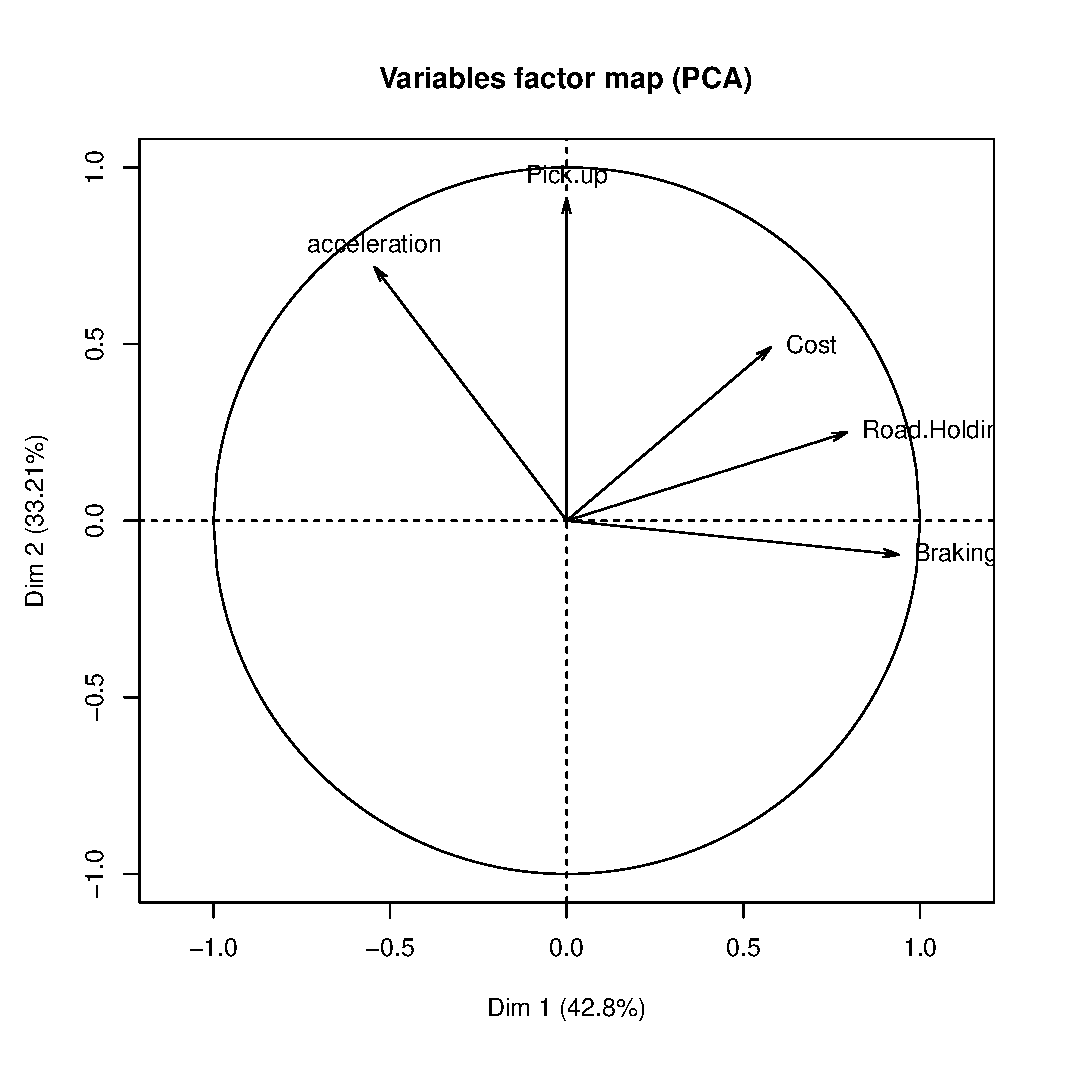
\includegraphics[width=7cm]{GRAPHE_THIERRY_FINAL_ACP.eps} 
    \caption{ACP 2D après bruitage de Cost par rapport à Road.Holding. Paramètre=(Newdata,1,5,0.4,100,500)} 
\end{figure} 

Le résultat semble assez bruité et donc satisfaisant.
Il serait intéressant de savoir maintenant si nous avons conservé la structure de notre réseaux bayésien appris sur le jeux initiale Fig.{figdepart}.


En apprenant un  réseaux sur le jeux de données modifié par $Cost/acceleration$ et $Cost/Road.Holding$:


\begin{figure}[H] 
    \center 
    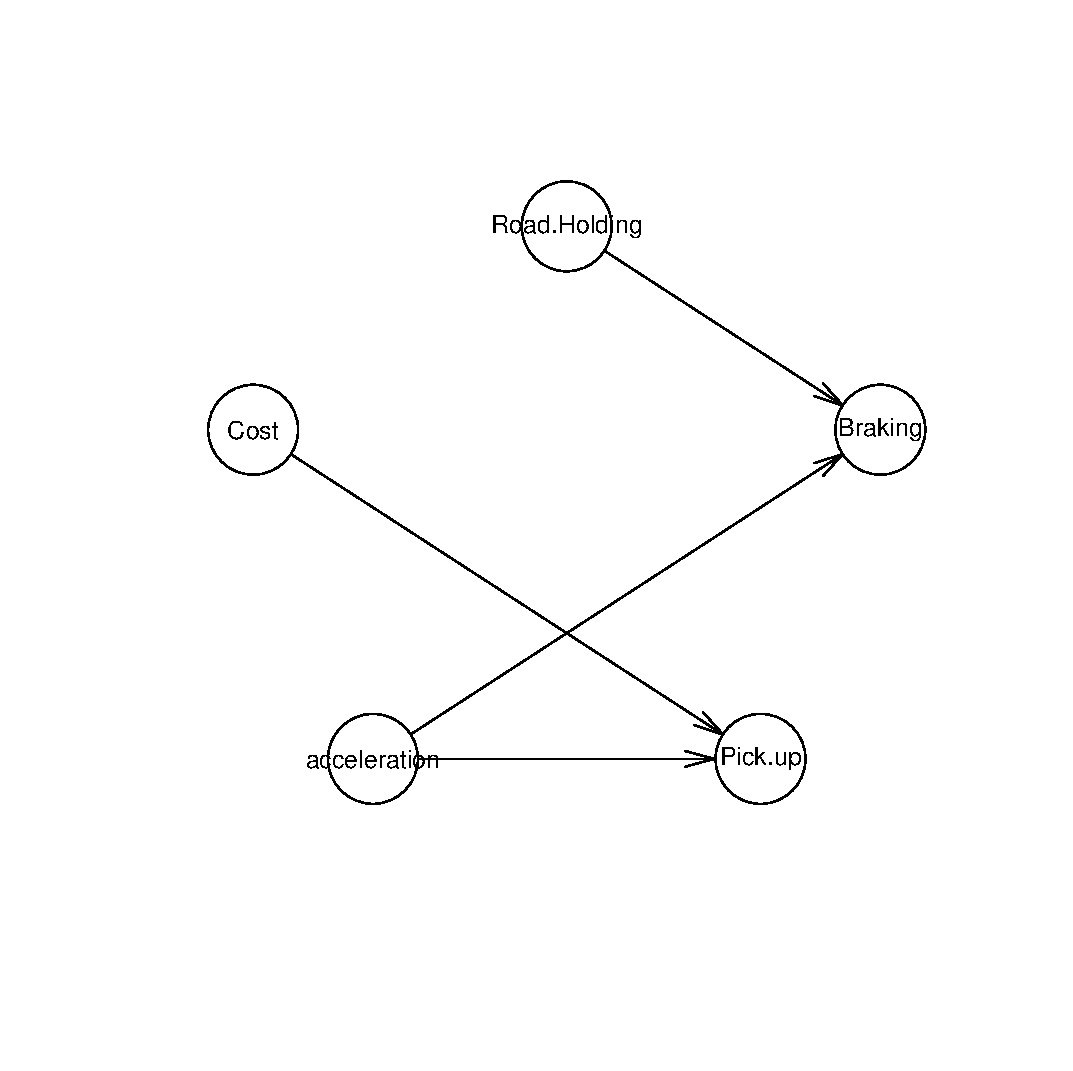
\includegraphics[width=8cm]{GRAPHE_FINAL_THIERRY.eps} 
    \caption{Réseaux obtenu après bruitage de Cost par rapport à Road.Holding. Paramètre=(Newdata,1,5,0.4,100,500)} 
\label{fig_network}
\end{figure} 


\textbf{Commentaires}:


\begin{itemize}
\item Il faut procéder pas à pas et la méthode peut assez vite devenir laborieuse si l'on veut ajuster de nombreuse corrélations. Nous verrons par la suite qu'il est bien plus intéressant d'agir sur les paramètres d'un réseaux. 


\item Lorsque nous avons étudié la robustesse par faible bruitage, on a pu constater que le réseaux était fort sensible au variations appliquées sur le jeux de données appris. Il est donc logique que la modification des corrélations par grand bruitage aura un impact directe sur le réseaux, ceci est bien  illustrée par le réseaux de la Fig.\ref{fig_network}.
\end{itemize}

























\newpage
\subsubsection{Validation des valeurs générées}

Nous allons vérifier que les individus générés sont proches des individus initiaux.

Remarquons dans un premier temps  que les centres de gravités et les écarts-types résiduels des deux nuages de points associé aux deux jeux de données sont approximativement les mêmes dans  l'espace total de \textbf{5 dimensions} :
\[
\left\lbrace 
\begin{array}{lcl} 
\vec{G_{14}}\equiv (17229.142857   ;29.533571 ;36.328571 ; 2.020000 ; 2.232143) \\ \\
\vec{G_{1000}}\equiv (17245.836938;29.56437; 36.377949; 2.010839;2.231846)\\  \\
\vec{Sd_{14}}\equiv (2025.0149803;0.8208402; 1.7847338; 0.3808695 ;0.5839544) \\  \\
\vec{Sd_{1000}}\equiv  (2048.1221306 ; 0.8075471 ;1.7380689; 0.3618966; 0.5732251)\\  \\

\end{array}\right.
\]


Avant de procéder à une comparaison visuel, nous allons exposer les valeurs propres, les vecteurs propres normalisés ainsi que la quantité d'information reprise par les valeurs propres. 

Ces grandeurs sont déduite d'une analyse en composantes principales \textbf{normalisée} appliquée au jeux de données obtenu après génération de 1000 valeurs:
\[
\left\lbrace 
\begin{array}{lcl} 
\lambda_{1}= 2.1756706  &&       \vec{x}_{1}\equiv (0.4680006 ; -0.5639231;-0.3943820 ;0.5032369  ;    0.2327694 )  \\ \\
\lambda_{2}= 1.4607291     &&     \vec{x}_{2}\equiv ( 0.3146065 ; -0.2659459  ;-0.2796647 ;-0.4737890; -0.7263657 )     \\ \\

\lambda_{3}=  0.7460901  &&       \vec{x}_{3}\equiv ( -0.53407177 ;  0.13765802; -0.83183232 ; -0.02691673 ; 0.05610799 )  \\ \\

\lambda_{4}=   0.4293234  &&   \vec{x}_{4}\equiv ( 0.6157297;0.5730986; -0.2664426; -0.3049791 ; 0.3583728 )\\ \\

\lambda_{5}=   0.1881869 &&   \vec{x}_{5}\equiv ( -0.13282501;-0.51368452; 0.05756557;-0.65462953; 0.53538034)\\ \\

\end{array}\right.
\]
 
\underline{Qualité de l'information}:

$$\delta=\frac{(\lambda_{1}+\lambda_{2})}{(\lambda_{1}+\lambda_{2}+\lambda_{3}+\lambda_{4}+\lambda_{5})}=  0.7272799$$

La qualité d'information de $\approx$72 $\%$  est insuffisante, c'est pour cela que nous allons utiliser le troisièmes vecteurs propres afin d'avoir une comparaison plus fiable.

La qualité de l'information devient alors:

$$\delta=\frac{(\lambda_{1}+\lambda_{2}+\lambda_{3})}{(\lambda_{1}+\lambda_{2}+\lambda_{3}+\lambda_{4}+\lambda_{5})}=   0.8764979$$

Ce qui est plus acceptable.


\newpage
Nous utilisons maintenant une ACP 3D pour obtenir une représentation géométrique de la variabilité des deux jeux de données.
Les deux représentations  sont obtenus par la projection des nuages de points des deux jeux de données sur les plans principaux formés par les vecteurs propres décrits précédemment.

\begin{figure}[H]
\fbox{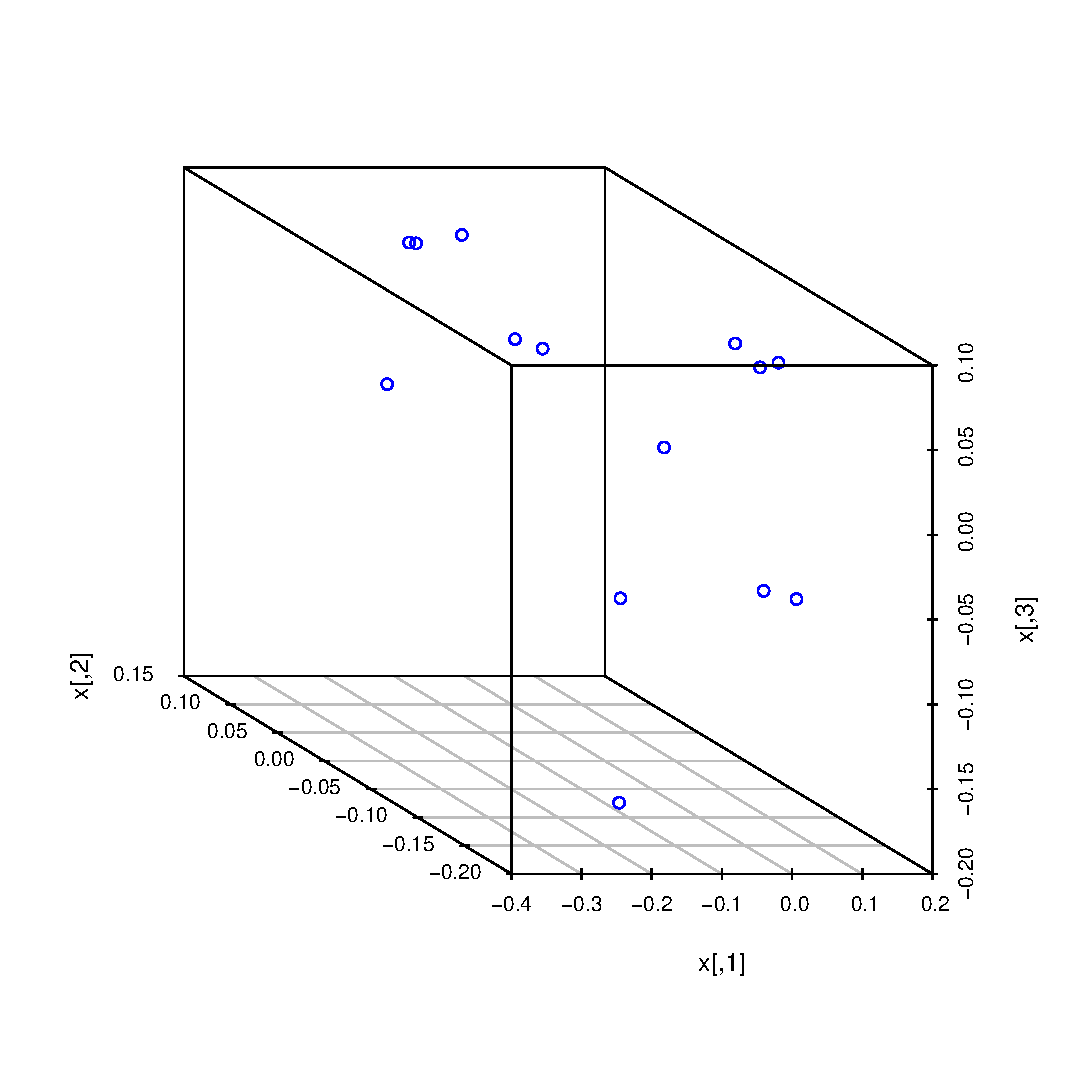
\includegraphics[width=6cm]{cubedata.eps}}\hfill
\fbox{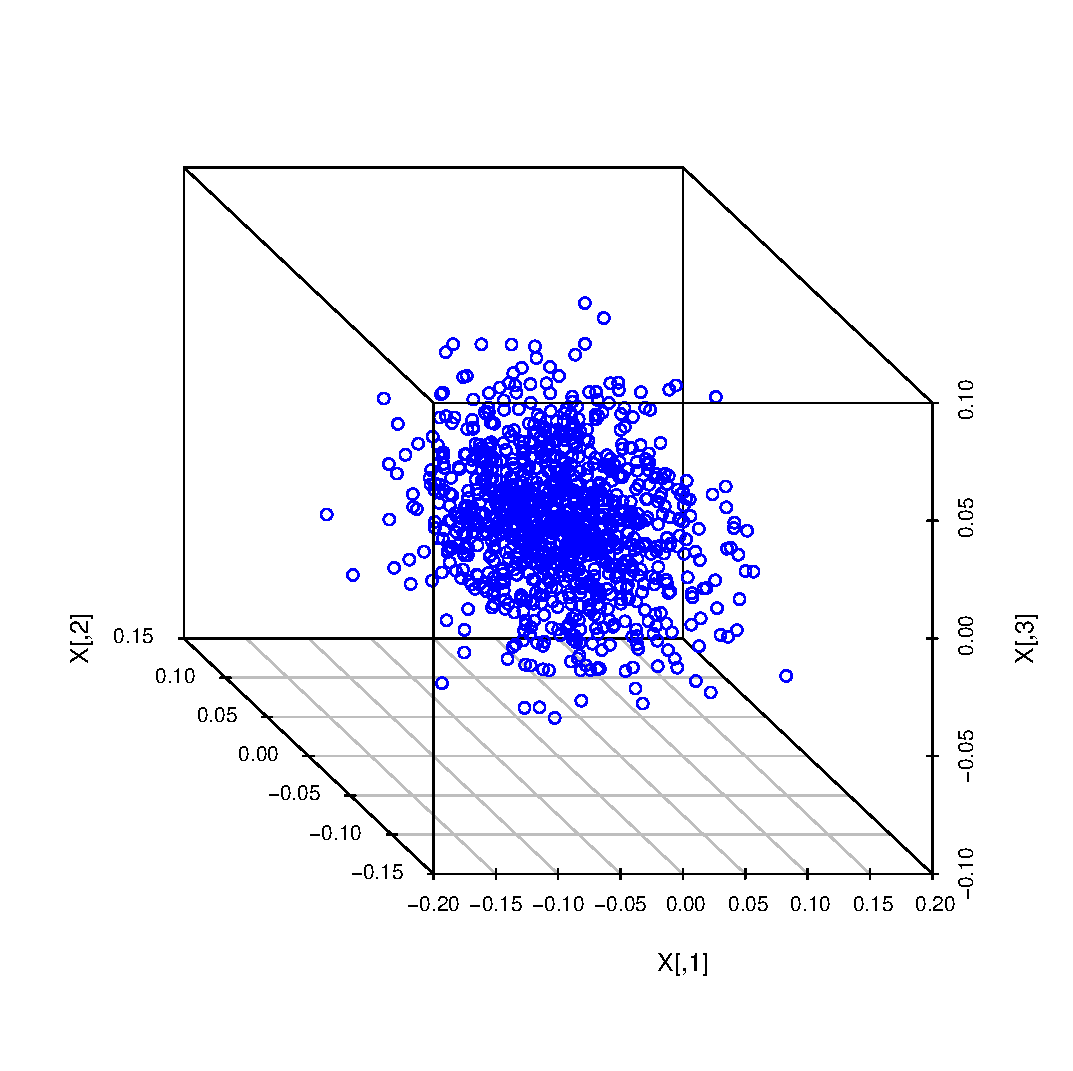
\includegraphics[width=6cm]{cubegener.eps}}
\caption{Projection du jeux de données initial et du jeux de 1000 valeurs dans le sous-espace munis du repère $(\vec{G},\vec{x_{1}},\vec{x_{2}},\vec{x_{3}})$}\label{fig:somefiglabel}
\end{figure}


Afin de mieux voir la proximité des deux jeux de données, nous projetons les deux nuages de points sur les 3 plans principaux formé par les vecteurs $(\vec{x_ {1}},\vec{x_{2}},\vec{x_{3}})$:
\begin{figure}[H]
\includegraphics[width=6cm]{proj12data.eps}\hfill
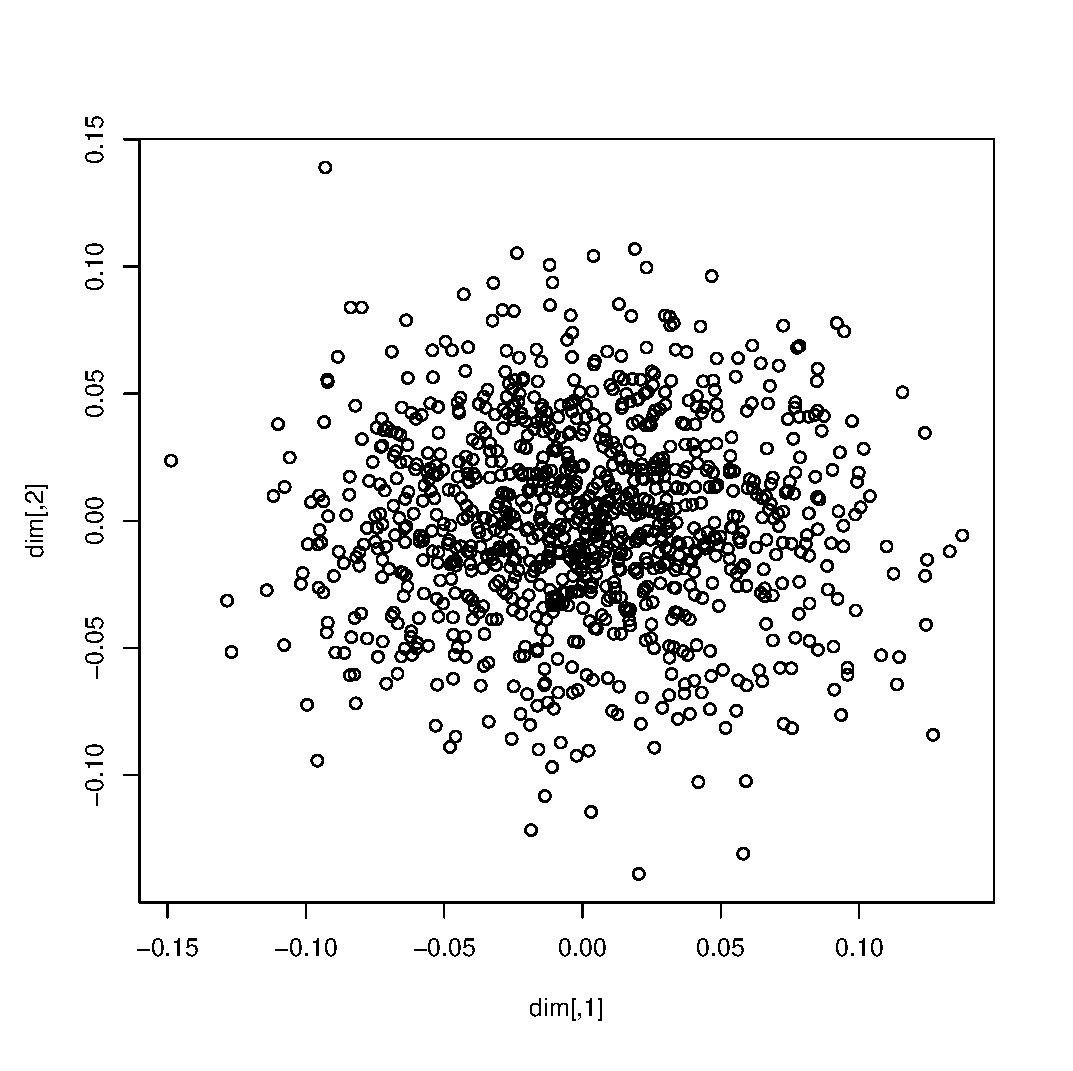
\includegraphics[width=6cm]{proj12gener.eps}
\caption{Projection du jeux de données initial et du jeux de 1000 valeurs sur le plan $(\vec{G},\vec{x_{1}},\vec{x_{2}})$}\label{fig:somefiglabel}
\end{figure}

\begin{figure}[H]
\includegraphics[width=6cm]{proj13data.eps}\hfill
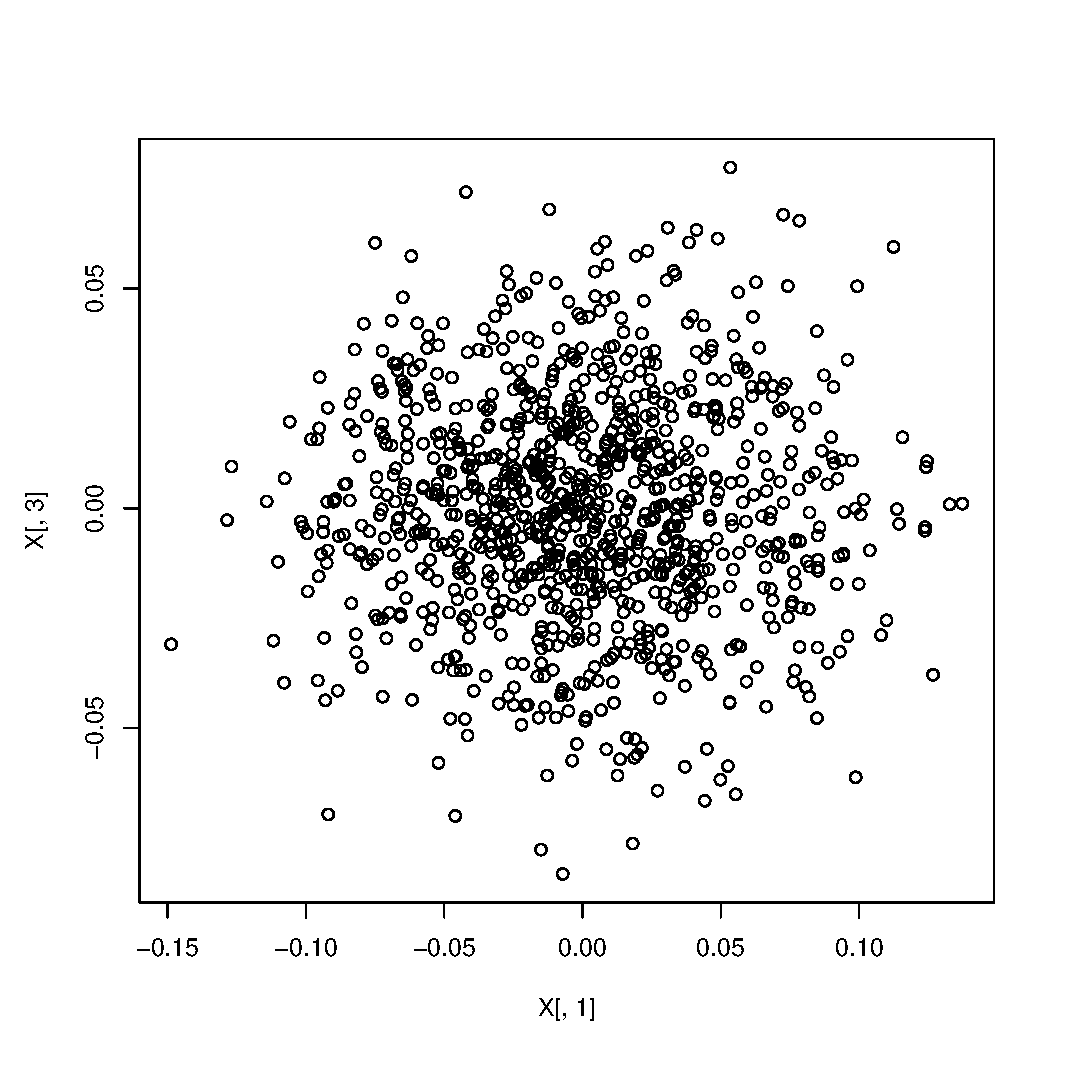
\includegraphics[width=6cm]{proj13gener.eps}
\caption{Projection du jeux de données initial et du jeux de 1000 valeurs sur le plan $(\vec{G},\vec{x_{1}},\vec{x_{3}})$}\label{fig:somefiglabel}
\end{figure}

\begin{figure}[H]
\includegraphics[width=5cm]{proj23data.eps}\hfill
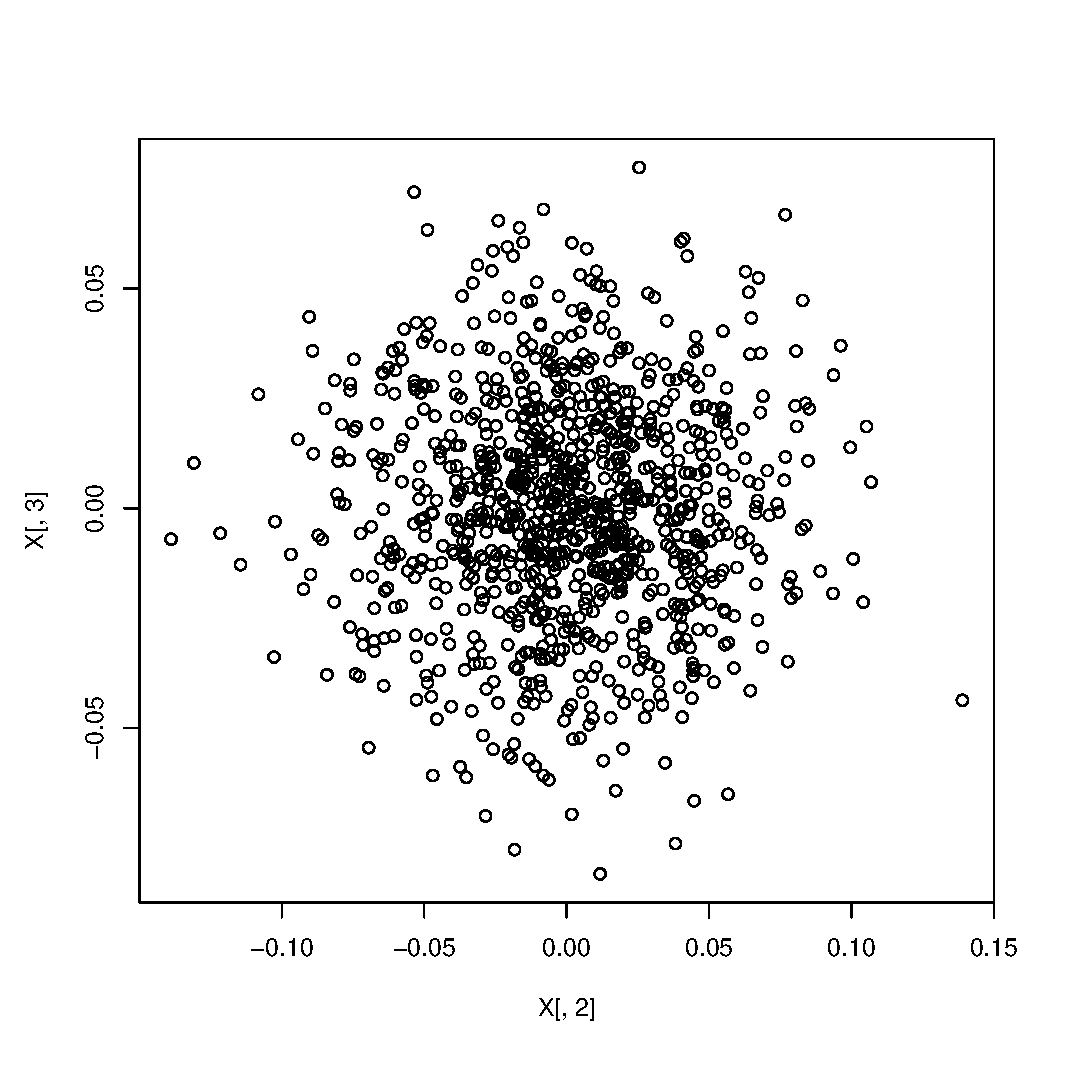
\includegraphics[width=5cm]{proj23gener.eps}
\caption{Projection du jeux de données initial et du jeux de 1000 valeurs sur le plan $(\vec{G},\vec{x_{2}},\vec{x_{3}})$}\label{fig:somefiglabel}
\end{figure}

\newpage

Le diagramme en boîte des nuages de points pour les 5  dimensions sont  représentés ci-dessous:
\begin{figure}[H]
\fbox{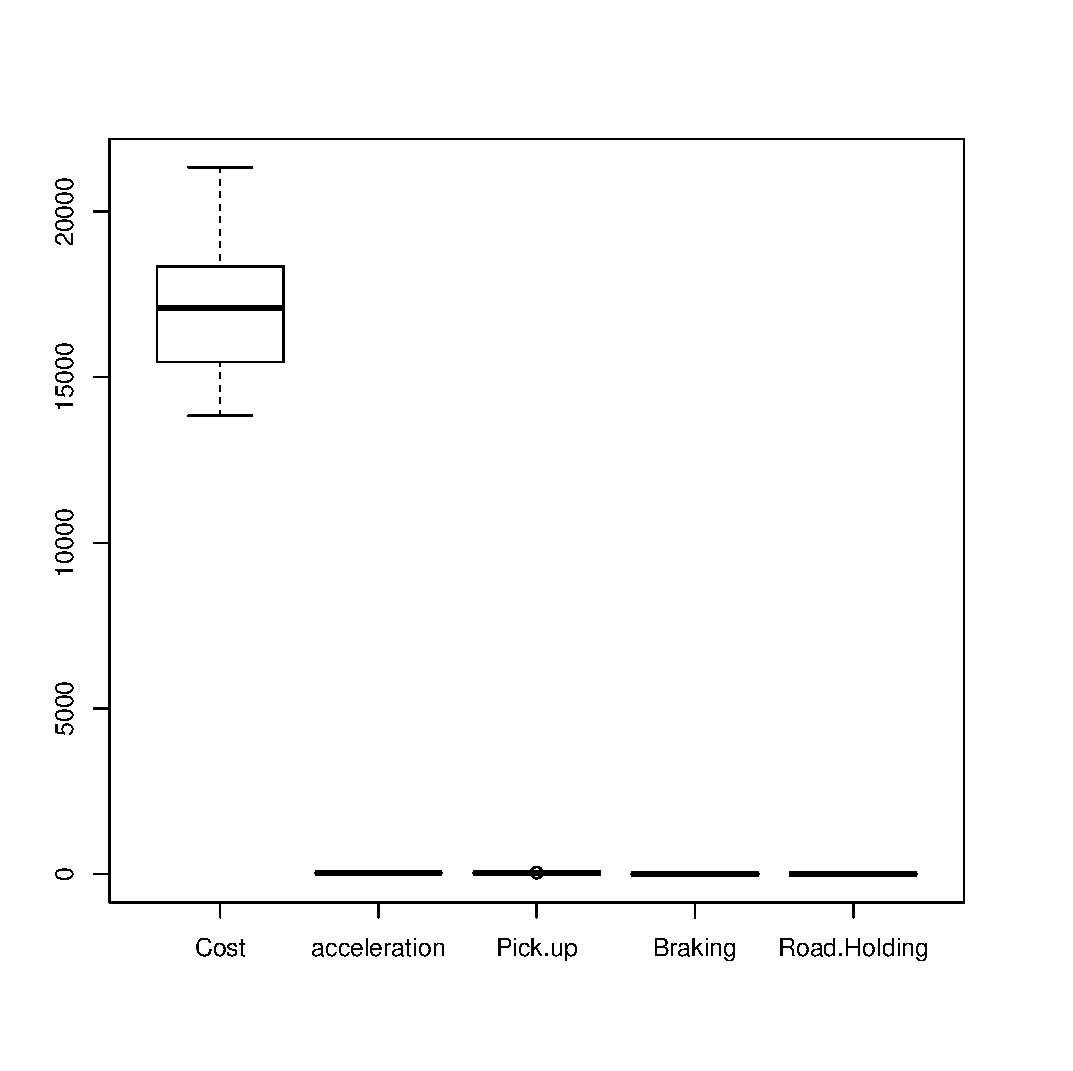
\includegraphics[width=6cm,height=5cm]{mousdata.eps}}\hfill
\fbox{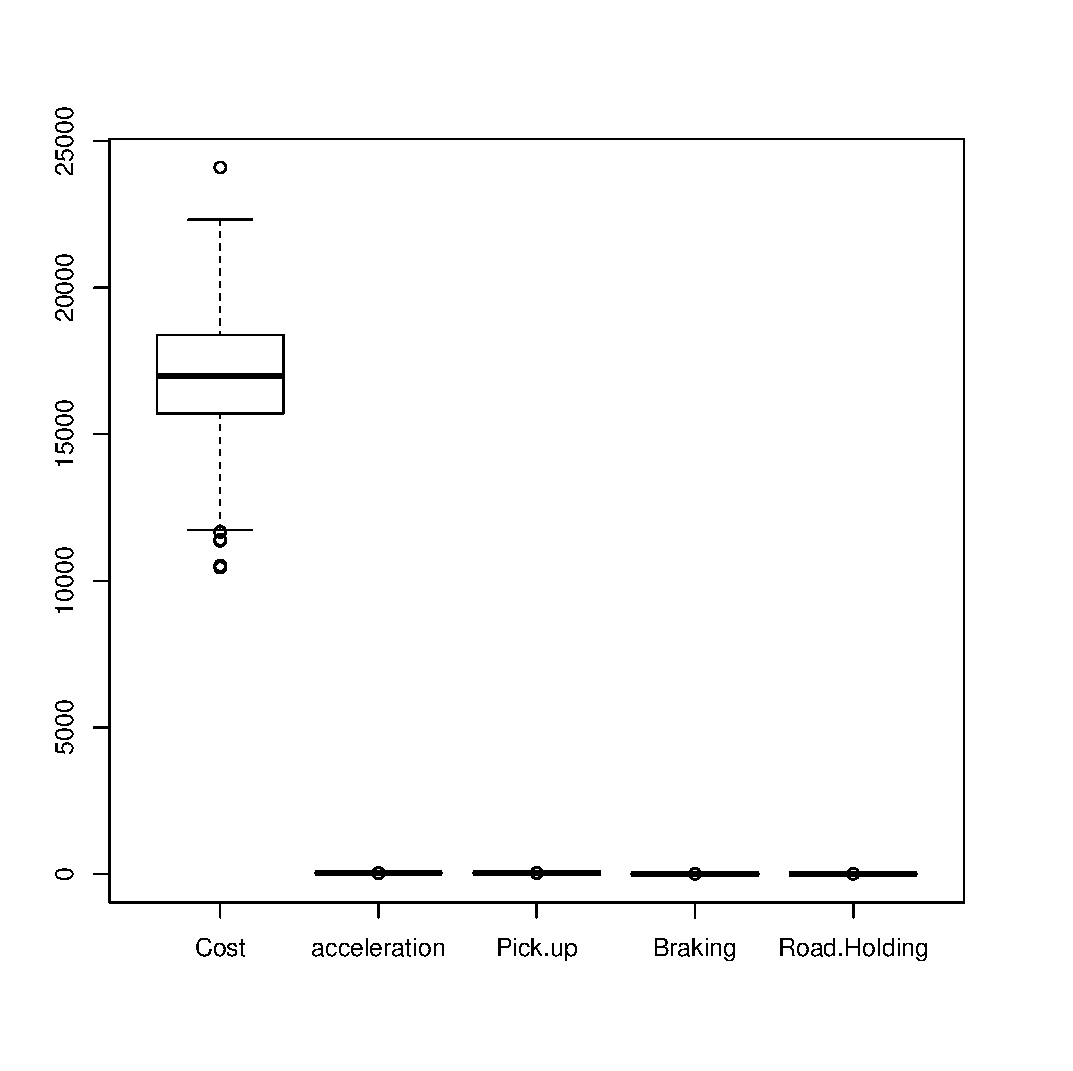
\includegraphics[width=6cm,height=5cm]{mousgener.eps}}
\caption{Représentation par un diagramme en boîte du jeux de données initial(gauche) et du jeux de données obtenu par génération de 1000 valeurs(droite)}\label{fig:somefiglabel}
\end{figure}

\begin{figure}[H]
\fbox{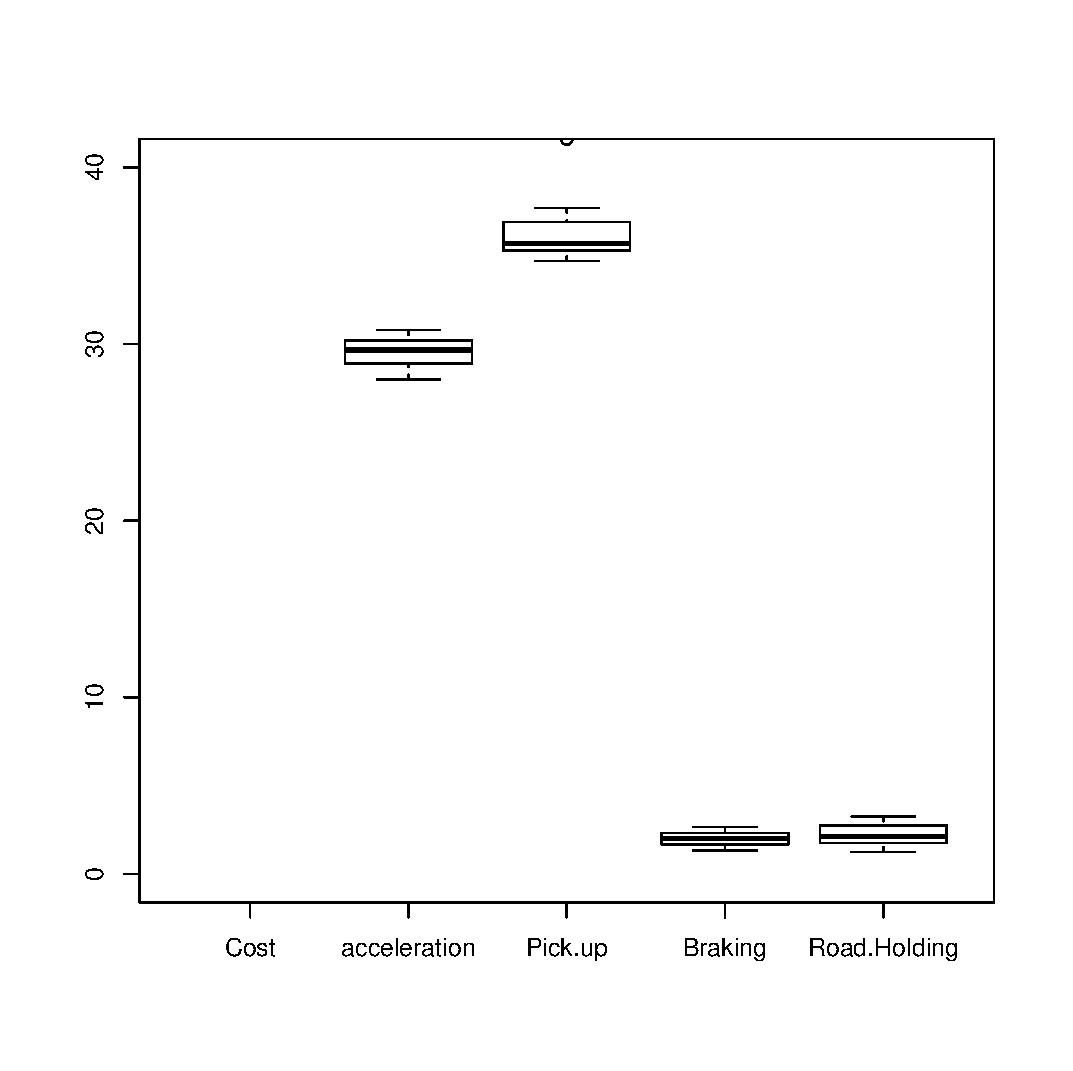
\includegraphics[width=6cm,height=5cm]{boxplotzoomdata.eps}}\hfill
\fbox{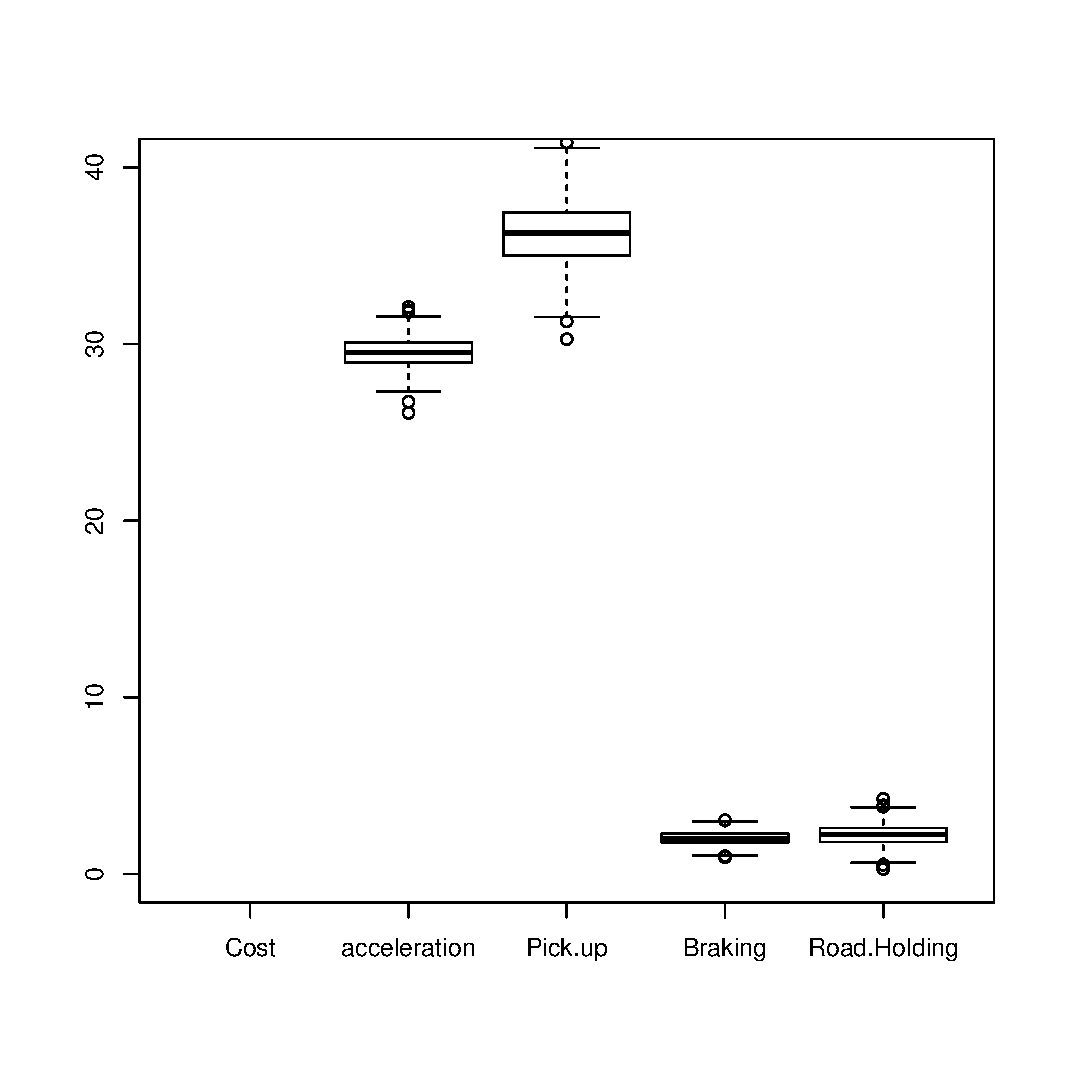
\includegraphics[width=6cm,height=5cm]{boxplotzoomgener.eps}}
\caption{Représentation par un diagramme en boîte du jeux de données initial(gauche) et du jeux de données obtenu par génération de 1000 valeurs(droite) avec un zoom }\label{fig:somefiglabel}
\end{figure}




\newpage
\section{Création de jeux de données}

\subsection{Introduction}

Dasn cette section, nous retrouverons trois grandes partie.
\begin{itemize}
\item La première section consistera à exposer la modélisation mathématique (OLS) qui est utilisée pour générer nos données.
Ce premier point se terminera par la présentation du système de paramétrisation d'un réseau.

\item La deuxième section traitera l'ajustement des paramètres d'un réseau. Comme nous l'avons déjà dit, l'ajout de bruit brut sur un jeux de données est une méthode assez  laborieuse pour décorréler les critères . Il est plus aisé d'agir sur les paramètre du réseau, cette section nous montrera alors l'impact des ajustements des  paramètres sur le bruitage des données.


\item La dernière section consistera à créer un jeux de données basée sur les données initial d'un petit jeux de données. 
La création du jeux sera basée sur le problème concernant l'achat d'une voiture étudié dans la section d'apprentissage.
Un autre exemple est présenté en annexe \ref{creat_guitare}.
Nous partirons du modèle de dépendance et d'indépendance du problème pour aboutir à la construction d'un réseaux permettant de générer des données réalistes. 

\end{itemize}

A l'aide de la première section on trouvera aussi   en annexe \ref{creat_stat} une manière de créer un jeux contraint à répondre à des critères statistiques pré-établit.

La construction d'un réseaux se fait en 3 points :

\begin{enumerate}


\item  \underline{\textbf{Modélisation en formule de dépendances et d'indépendances mathématique}}: {\\}


La modélisation d'un problème consiste à mettre un ensemble de variables sous forme de relations de dépendances $\{\not\ci \}$ et d'indépendances $\{\ci\}$.

Cela implique bien entendu que le problème doit être modélisable en \textbf{réseaux bayésiens}.
Il existe des cas où la modélisation n'est malheureusement pas possible.

Ex:
$$\left\lbrace 
\begin{array}{lcl} 
A\not\ci B \Longrightarrow A\ci B|D\\
A\ci D \Longrightarrow  A\not\ci D|E\\
\end{array}\right.$$

La première relation impose que le triplet $(A,D,B)$ ne peut être qu'une V-structure, il existe donc forcément un arc $A \longrightarrow D$ ce qui est en contradiction avec la deuxième relation
Nous dirons alors que:\textit{les relations sont incompatible en modélisation bayésienne.} 

Dans le cas où la modélisation bayésienne est réalisable, nous distinguons deux types de relations:
\begin{itemize}
\item \textbf{-Les relations directes} qui sont des relations binaires de dépendances ou d'indépendances du types:

\[
\left\lbrace 
\begin{array}{lcl} 
A\not\ci B\\ 
\text{ou}\\ 
A\ci B
\end{array}\right.
\]

\item \textbf{La relation indirecte} qui sont des relations binaires impliquant une relation tertiaire effectuant la transformation: $(\ci,\not\ci)\Longrightarrow (\not\ci,\ci)$.
Nous aurons alors dans ce cas des relations du types:

\[
\left\lbrace 
\begin{array}{lcl} 
A\not\ci B \Longrightarrow A\ci B|C\\  
\text{ou} \\ 
A\ci B \Longrightarrow A\not\ci B|C 
\end{array}\right.
\]
\end{itemize}


\item  \underline{\textbf{ Réalisation de la structure}}:{\\}

La première remarque réside sur le fait que les différentes étapes de constructions ne pourront jamais introduire de cycles.

Les relations directes seront dans un premier temps représentées par des arrêtes dans un graphe non-orienté.

Les relations indirectes vont alors orienter le graphe en transformant les arrêtes $(A,B)$ en V-structures, structure séries ou en structure divergentes de la façon suivante:
\[
\left\lbrace 
\begin{array}{lcl} 
\text{  V-structure  }\equiv\{ A\not\ci B \Longrightarrow A\ci B|C \}  \\  \\
\text{ Structure séries ou divergentes }\equiv \{ A\ci B \Longrightarrow A\not\ci B|C \}
\end{array}\right.
\]
Nous plaçons d'abord les V-structures dans le graphe car elle ne possède aucun degré liberté, ce qui n'est pas le cas d'une structure en série qui pourra souvent être remplacé par une structure divergente et réciproquement.

Nous dirons que le problème est \textit{exacte} si le modèle des dépendances et d 'indépendances fige toutes les orientations du graphe.

 Dans le cas contraire , nous aurons des degrés de liberté sur le graphe répondant au modèle et nous choisirons arbitrairement les orientations restantes.

\item  \underline{\textbf{ Paramétrisation du réseaux}}:{\\}

Nous savons que la factorisation de Verma definit en \ref{factoverma} fait intervenir les probabilités conditionelles.
Un noeud $Y$ ayant pour parents $\{X_{1},...,X_{n}\}$ nous impose de connaître une probabilité $P(Y|X_{1},...,X_{n})$, pour cela il faut décrire la variable $Y$ exogène comme étant la réponse des variables $\{X_{1},...,X_{n}\}$ endogènes.

Nous allons approcher $Y\approx f(X_{1},...,X_{n})$  par une régréssion linéaire du type

$$Y\approx\sum_{i=1}^{n}a_{i}.X_{i}+b$$


Les coefficients $a_{i=1..n}$ et $b_{i=1...n}$, à paramétrer,  sont respectivement les coefficients de régressions et d'intercepetions de la régression linéaire.Un paramètre d'écart-type $\eta(0,S_{d})$ provoquant le bruit autour de la régréssion est aussi à fixé.

Dans cette section nous exposerons deux manières  de paramétriser le réseaux:

\begin{itemize}
\item La première paramétrisation se fait en utilisant les paramètres des régression d'un petit jeux de données pour ensuite les transférer dans un réseaux afin de générer des données réalistes. Cette paramétrisation est présenté dans cette section.

\item La deuxième paramétrisation consistera à exposer une technique mathématique permettant de paramétriser un réseaux dont les données générés vérifieront les contraintes suivantes:
 

-Le jeux de données doit vérifier un modèle de dépendance et d'indépendance.

-Chaque vecteurs colonnes du jeux de données aura une moyenne, un écart-type imposées.



Cette deuxième paramétrisation est présenté en annexe \ref{creat_stat}.
\end{itemize}

\end{enumerate}
\newpage
\subsection{Système de paramétrisation }

\subsubsection{Introduction}
L'objectif de cette  partie est de présenter le système de paramétrisation que nous allons utiliser en fin de section et en annexe \ref{creat_stat}.

Dans le point concernant l'apprentissage,  nous avons  généré des valeurs à l'aide d'une fonction automatique. La génération automatique dissimule la paramétrisation du réseaux. Le but est alors ici d'exposer  le système qui dimensionne le réseaux bayésien. Le problème d'ajustement sera lui présenté à la section suivante.



Rappelons tout d'abord qu'un ensemble de vecteurs aléatoires générés $\vec{X_{1}},\vec{X_{2}},...,\vec{X_{n}}$ de longueur $k$ qui suit une distribution gaussienne multi-variable de moyenne $\vec{\mu}$ et de matrice variance-covariance $\Sigma$ vérifie le principe d'échantillonnage suivant:

Si $\overline{\overline{X}}$ et $S$ correspondent respectivement à la moyenne et la matrice variance-covariance de l'échantillon alors :
\begin{itemize}
  \item $\overline{\overline{X}}$ suit une normal multivariable $\eta(\overline{\mu},\frac{\Sigma}{n})$.
  \item $S$ suit une distribution de Wishart $Wish(\frac{S}{n-1},\Sigma)$
\end{itemize}

Où $Wish(\frac{S}{n-1},\Sigma)$ est une distribution dite de \textit{Wishart} de $n$ degré de liberté .Vous pourrez trouver plus d'information concernant cette distribution dans l'ouvrage de référence \textit{Optimal statistical décision} de Morris H.De Groot.
D'après les expressions ci-dessus, il va de soi que nous ne générons jamais   un jeux possédant exactement la même moyenne et la même matrice variance-covariance  que la population, mais il y'a cependant  une convergence du vecteur moyenne et de la matrice variance-covariance de l'échantillon par rapport à la propulation. On obtiendra de bonne valeurs pour une génération de 1000 individus.

Le système de paramétrisation sera présenté sur base de la connaissance d'un vecteur moyenne  $\vec{\mu}$, d'écart-type $\vec{S_{d}}$ et d'une matrice variance-covariance $S$ associés au jeux de données. 






On considère durant toute cette section que l'on a un jeux de données possédant $n$ critères notés $\{C_{j}\}_{j=1,...,n}$

Nous faisons l'hypothèse que la modélisation de dépendance et d'indépendance est forcément \textit{compatible} en réseaux bayésien. 
Le problème possède alors au moins une solution $B(C_{j},\xi)$ ( où les $\xi$ sont les arcs du réseaux bayésien).

\newpage
\subsubsection{Modèle de dépendance et d'indépendance à partir de données statistiques}

Nous avons à notre disposition le problème de dépendance et d'indépendance suivant:

$\{C_{j}\}_{j=1,...,n}\Longrightarrow\left\lbrace 
\begin{array}{lcl} 
C_{k} \not\ci C_{l} \text{     avec } k \ne l\\ \\
C_{m} \ci C_{n} \text{     avec } m\ne n\\ \\
C_{p}\not\ci C_{q} \Longrightarrow C_{p}\ci C_{q}|C_{r} \text{   avec  }  p\ne q\ne r      \\ \\
C_{u}\ci C_{v} \Longrightarrow C_{u}\not\ci C_{v}|C_{w}\text{   avec } u\ne v\ne w\\ \\   
 \end{array}\right.$

avec $\{k,l,m,n,p,q;u,v,w\}\in \{1,...,n\}$.

Nous ne traitons pas le problème de compatibilité car le système est supposé \textit{compatible} par hypothèse.
 On obtient donc au minimum une solution bayésienne pour le modèle de dépendance et d'indépendance.
Parmi les réseaux solutions, nous allons en choisir un et nous le notons $B(C_{j},\xi)$.

Considérons les données statistiques de départ définis ci-dessous:

$\left\lbrace 
\begin{array}{lcl} 
\vec{G}\equiv (\mu_{c_{1}},\mu_{c_{2}},...,\mu_{c_{n}})\\ \\ 
\vec{Sd} \equiv (S_{c_{1}},S_{c_{2}},...,S_{c_{n}})\\ \\  \\ \\
\overline{\rho}=\begin{pmatrix}
1&\ \ \rho_{c_{1}c_{2}}&\ \ \rho_{c_{1}c_{3}}&\ \ \rho_{c_{1}c_{4}}&.................... &\ \ \rho_{c_{1}c_{n}}\\ 
\rho_{c_{2}c_{1}}&\ \ 1&\ \ \rho_{c_{2}c_{3}}&\ \ \rho_{c_{2}c_{4}}&....................&\ \ \rho_{c_{2}c_{n}}\\ 
\rho_{c_{3}c_{1}}&\ \ \rho_{c_{3}c_{2}}&\ \ 1&\ \ \rho_{c_{3}c_{4}}&....................&\ \ \rho_{c_{3}c_{n}}\\ 
...&...&...&...&...&...  \\ 
...&...&...&...&...&...  \\ 

\rho_{c_{n}c_{1}}&\ \ \rho_{c_{n}c_{2}}&\ \ \rho_{c_{n}c_{3}}&\ \ \rho_{c_{n}c_{4}}&....................&\ \ 1\\ 

\end{pmatrix}
\end{array}\right.$


On peut exprimer sans problème la matrice variance-covariance en fonction de nos données  :



$\\ \\  S=\begin{pmatrix}
S_{c_{1}}^2&\ \ \rho_{c_{1}c_{2}}.S_{c_{1}}.S_{c_{2}}&\ \ \rho_{c_{1}c_{3}}.S_{c_{1}}.S_{c_{3}}&\ \ \rho_{c_{1}c_{4}}.S_{c_{1}}.S_{c_{4}}&.................... &\ \ \rho_{c_{1}c_{n}}.S_{c_{1}}.S_{c_{n}}\\ 
\rho_{c_{2}c_{1}}.S_{c_{2}}.S_{c_{1}}&\ \ S_{c_{2}}^2&\ \ \rho_{c_{2}c_{3}}.S_{c_{2}}.S_{c_{3}}&\ \ \rho_{c_{2}c_{4}}.S_{c_{2}}.S_{c_{4}}&.................... &\ \ \rho_{c_{2}c_{n}}.S_{c_{2}}.S_{c_{n}}\\ 
\rho_{c_{3}c_{1}}.S_{c_{3}}.S_{c_{1}}&\ \ \rho_{c_{3}c_{2}}.S_{c_{3}}.S_{c_{2}}&\ \  S_{c_{3}}^2      &\ \ \rho_{c_{3}c_{4}}.S_{c_{3}}.S_{c_{4}}&.................... &\ \ \rho_{c_{3}c_{n}}.S_{c_{3}}.S_{c_{n}}\\ 
...&...&...&...&...&...  \\ 
...&...&...&...&...&...  \\ 

\rho_{c_{n}c_{1}}.S_ {c_{n}}.S_{c_{1}}&\ \ \rho_{c_{n}c_{2}}.S_ {c_{n}}.S_{c_{2}}&\ \ \rho_{c_{n}c_{3}}.S_ {c_{n}}.S_{c_{3}}&\ \ \rho_{c_{n}c_{4}}.S_ {c_{n}}.S_{c_{4}}&....................&\ \ S_{c_{n}}^2\\ \\ 

\end{pmatrix}$


Cette matrice peut donc être calculé et nous pouvons obtenir les différentes covariances:

$$S_ {c_{i}c_{j}}=\rho_{c_{i}c_{j}}.S_{c_{i}}.S_{c_{j}}$$

Les $S_ {c_{i}c_{j}}$ serviront  à paramétriser notre réseau.


\newpage
\subsubsection{Paramétrisation du réseaux bayésien}

La paramétrisation consiste à trouver les coefficients des régréssions linéaires: 
$$ Y_{c_{k}}\approx f(X_{c_{i}})$$ 
$C_{k}$ correspond à un noeud ayant pour parents $C_{i}$ et $ Y_{c_{k}}$ sont les variables exogènes expliquées par les variables endogènes $X_{c_{i}}$. 

$Y_{c_{k}}$ exprime donc les valeurs prises par les critères $C_{k}$ en réponse aux valeurs prises par $C_{i}$.

Les  régressions linéaires seront du type constantes, simples ou multiples suivant respectivement que le noeud $Y_{c_{k}}$ ne possède pas de parents, possède un parent ou possède deux parents.

Nous allons maintenant expliciter les 3 différentes régressions:

\begin{enumerate}
\item  \textbf{Régression constante associé à un noeud $C_{k}$ ne possédant pas de parents:}

Dans ce cas la constante prise est la moyenne sur le critère courant $C_{k}$:

$$Y_{c_{k}}\approx \mu_{c_{k}}$$

\item \textbf{La régression simple associé à un noeud $C_{k}$ possédant un parent $C_{i}$:}

Dans ce cas on a une expression du type:

$$Y_{c_{k}}\approx \alpha.X_{c_{i}}+\beta$$

Les paramètres $\alpha$ et $\beta$ seront évalués par: 
\[
\left\lbrace 
\begin{array}{lcl}
\alpha=\frac{S_{c_{k}c_{i}}}{S_{c_{i}}^2}\\ \\

\beta=\mu_{c_{k}}-\alpha.\mu_{c_{i}}\\ \\
\text{Avec   } \\ \\
S_{c_{k}c_{i}}=\rho_{c_{k}c_{i}}S_{c_{k}}S_{c_{i}}
\end{array}\right.
\]
\newpage
\item \textbf{La Régression linéaire multiple à deux variables associé à un noeud $C_{k}$ possédant deux parents $C_{i}$ et $C_{j}$}


Nous avons ici typiquement une V-structure.

 $Y_{c_{k}}\approx f(X_{c_{i}})$ est évalué de la façon suivante:

$$Z_{c_{k}}\approx \alpha.X_{c_{i}}+\beta.Y_{c_{j}}+\gamma$$


Nous admettons que la somme des moindres carrée à deux variables pour $m$ individus impose de manière général la relation suivante:

$\begin{pmatrix}
\gamma\\ \\
\alpha\\ \\
\beta\\ \\
\end{pmatrix}$
$=\begin{pmatrix}
m&\sum_{i=1}^{m}X_{i}&\sum_{i=1}^{m}Y_{i}\\ \\
\sum_{i=1}^{m}X_{i}&\sum_{i=1}^{m} X_{i}^2&\sum_{i=1}^{m}X_{i}.Y_{i}\\ \\
\sum_{i=1}^{m}Y_{i}&\sum_{i=1}^{m}X_{i}.Y_{i}&\sum Y_{i}^2\\ \\
\end{pmatrix}^{-1}$
$.\begin{pmatrix}
\sum_{i=1}^{m}Z_{i}\\ \\
\sum_{i=1}^{m}X_{i}Z_{i}\\ \\
\sum_{i=1}^{m}Y_{i}Z_{i}\\ \\
\end{pmatrix}$

Si nous faisons intervenir les moyennes, les variances et covariances et que nous simplifions par la taille $m$:

$\begin{pmatrix}
\gamma\\ \\
\alpha\\ \\
\beta\\ \\
\end{pmatrix}$
$=\begin{pmatrix}
1&\mu_{c_{i}}&\mu_{c_{j}}\\ \\

\mu_{c_{i}}&S_{c_{i}}^{2}&S_{c_{i}c_{j}} \\ \\

\mu_{c_{j}}&S_{c_{i}c_{j}}&S_{c_{j}}^{2}\\ \\
\end{pmatrix}^{-1}$
$.\begin{pmatrix}
\mu_{c_{k}}\\ \\
S_{c_{i}c_{k}}\\ \\
S_{c_{j}c_{k}}\\ \\

\end{pmatrix}$

\end{enumerate}




\newpage
\subsubsection{Système de paramétrisation}
\begin{itemize}
\item Si on définit les sous-ensembles $\{C_{j}^{(0)}\}$,  $\{C_{j}^{(1)}\}$ et $\{C_{j}^{(2)}\}$ de $\{C_{j}\}_{j=1,...,n}$ comme étant respectivement les sous-ensembles de noeuds de degrés incidents égale à 0, 1 et 2.

\item Si nous notons  $\pi_{1}(C_{j}^{(2)})$ et  $\pi_{2}(C_{j}^{(2)})$ comme étant respectivement le premier et le deuxième parents de $C_{j}^{(2)}$ 

\item Si $\pi(C_{j}^{(1)})$ est noté comme étant l'unique parent de $C_{j}^{(1)}$.

\item Si nous notons  $\mu(C_{j})$, $S(C_{i},C_{j})$, $Y(C_{j})$ et $X(C_{j})$  à la place respectivement de  $\mu_{c_{j}}$,$S_{c_{i},c_{j}}$, $Y_{c_{j}}$ et $X_{c_{j}}$.
\end{itemize}

Le \textbf{système de paramétrisation} peut alors s'écrire comme:

$\left\lbrace 
\begin{array}{lcl} 
Y(C_{j}^{(0)})\approx\mu(C_{j}^{(0)}) \\ \\ \\

Y(C_{j}^{(1)})\approx \frac{ S(C_{j}^{(1)},\ \pi(C_{j}^{(1)}))}{S^{2}(\pi(C_{j}^{(1)}))}. X(\pi(C_{j}^{(1)}))+ \mu(C_{j}^{(1)})-\{\frac{ S(C_{j}^{(1)},\ \pi(C_{j}^{(1)}))}{S^{2}(\pi(C_{j}^{(1)}))}.\mu(\pi(C_{j}^{(1)}))\} \\ \\ \\

Y(C_{j}^{(2)})\approx\alpha_{1j}.\pi_{1}(C_{j}^{(2)})+\alpha_{2j}.\pi_{2}(C_{j}^{(2)})+\alpha_{3j}\\
\end{array}\right.\\ \\$


Les valeurs de $\alpha_{1,j},\alpha_{2,j}$ et $\alpha_{3j}$ s'obtiennent par le produit matriciel ci-dessous:


$\\ \\ \\ \begin{pmatrix}
\alpha_{3j}\\ \\
\alpha_{1j}\\ \\
\alpha_{2j}\\ \\
\end{pmatrix}
=\begin{pmatrix}
1&\mu(\pi_{1}(C_{j}^{(2)}))&\mu(\pi_{2}(C_{j}^{(2)}))\\ \\

\mu(\pi_{1}(C_{j}^{(2)}))&S^{2}(\pi_{1}(C_{j}^{(2)}))&S(\pi_{1}(C_{j}^{(2)}),  \pi_{2}(C_{j}^{(2)}))\\ \\

\mu(\pi_{2}(C_{j}^{(2)}))&S(\pi_{1}(C_{j}^{(2)}),  \pi_{2}(C_{j}^{(2)})&S^{2}(\pi_{2}(C_{j}^{(2)}))\\ \\
\end{pmatrix}^{-1}
.\begin{pmatrix}
\mu(C_{j})\\ \\
S(\pi_{1}(C_{j}^{(2)}),C_{j})\\ \\
S(\pi_{2}(C_{j}^{(2)}),C_{j})\\ \\

\end{pmatrix}$



\newpage
\subsection{Ajustement des paramètres d'un réseaux bayésien}
\subsubsection{Introduction}
Le but de ce point est de proposer une méthode d'ajustement des  paramètres d'un réseau afin que le jeux de données  générés ait une \textit{proximité} par rapport à un jeux de données réaliste. La notion de \textit{proximité} entre deux jeux de données tient compte du fait que les deux jeux possèdent : 
\begin{itemize}
\item Les mêmes relations de dépendances et d'indépendances.
\item Des corrélations du même ordre de grandeurs.
\item Des moyennes $\vec{\mu}$ et des vecteurs écarts-types $\vec{S_{d}}$ dont les composantes ont des valeurs assez proches.

\end{itemize}
 
Ces critères de \textit{proximité} dépendent bien entendu de l'exigence que nous attribuons au jeux que l'on veut obtenir. Nous dirons alors que plus le jeux générés est proche du jeux de données initiales plus il sera de bonne  \textit{qualité}.

En pratique il est conseillé d'utiliser dans un premier temps le système de paramétrisation du jeux de données initiales pour générer notre jeux artificiel.

Nous procédons si nécéssaire à un ajustement provoquant la \textit{dilatation} ou la  \textit{contraction} des nuages de points obtenus autour des régression suivants les cas ou nous voulons soit \textit{diminuer} ou \textit{augmenter} les corrélations.

Les opération de \textit{dilatation} et de \textit{contraction} se font en jouant sur l'écart-type $\sigma$ intervenant dans le bruit $\eta(0,\sigma)$ des régressions.

Dans les points qui vont suivre, nous allons voir l'impact et l'accumulation des différents bruits $\eta(0,\sigma_{k})$ dans un réseau.


\subsubsection{Fonction de transfert, dilatation et contraction}

En partant d'un jeux de données de 1000 données générés reprenant les mêmes régressions que le jeux de données initial.
On obtient déjà un jeux de donnée de bonne \textit{qualité}.

Les jeux diffères souvent que sur l'ordre de grandeur des corrélations. Cette section analyse l'impact d'une modification du bruit $\eta(0,\sigma)$ sur les corrélations.


Avant de parler de la  \textit{dilatation} et de \textit{contraction} du point de vue mathématique, nous devons définir la fonction de transfert existante entre deux noeuds non-adjacents. 

Nous prenons tout d'abord le cas d'un noeud $C_{1}$ de départ ne possédant  pas de parents et un noeud $C_{n}$ final ne possédant pas d'enfants.

On s'intéressera par la suite à l'ajout d'une V-structure ou d'une structure divergente en présentant l'impact de celle-ci sur les corrélations.

\begin{enumerate}
\item \textbf{ Structure série en cascade:}

Considérons la structure série en cascade:

$$C_{1}\longrightarrow C_{2} \longrightarrow C_{3} ..............\longrightarrow C_{n}$$	

Dans cette situation, la fonction de transfert $H$ est définis comme étant  la régression globale $C_{m}=H(C_{n})$ .
Nous n 'avons pas mis  $X(C_{m})\approx H(X(C_{n}))$ car le bruit $\eta(0,\sigma)$ est cette fois-ci inclus dans le système de paramétrisation.

Nous noterons pour éviter d'alourdir les expressions $X_{n}$ à la place de $X(C_{n})$ et $\eta(\sigma_{n})$ à la place de $\eta(0,\sigma_{n})$

Nous devons maintenant  développer  cette fonction de transfert et pour cela nous allons partir du \textit{système de paramétrisation} appliquée à notre structure série en cascade:

\[
\left\lbrace 
\begin{array}{lcl}
X_{1}=\mu_{1}+\eta(\sigma_{1}) \\ \\
X_{n+1}=\alpha_{n+1}.X_{n}+\beta_{n+1}+\eta(\sigma_{n+1})\\ \\ 
\text{Avec}\\ \\

\alpha_{n+1}=\frac{S_{n+1, n}}{S_{n}^{2}}.\\ \\

\beta_{n+1}=\mu_{n+1}-\mu_{n}.\frac{S_{n+1, n}}{S_{n}^{2}} \\ \\

\end{array}\right.
\]




Après quelques itérés, on peut se rendre compte que la fonction de transfert :

$$X_{n}=H(X_{1})$$

peut s'écrire:

\[
\left\lbrace 
\begin{array}{lcl}

X_{n}=\frac{A_{1}.S_{n}}{S_{1}}.X_{1}+\{  (\sum_{k=2}^{n-1}  \frac{A_{k}.S_{n}}{S_{k}}.\beta_{k})+\beta_{n}\}+\{(\sum_{k=2}^{n-1}\frac{A_{k}.S_{n}}{S_{k}}.\eta(\sigma_{k}))+\eta(\sigma_{n})                                                                                   \}    \\ \\      

A_{k}=\Pi_{i=k}^{n-1} \ \rho_{i,i+1}\\ \\
\beta_{k}=\mu_{k}-\mu_{k-1}.\frac{S_{k,k-1}}{S_{k-1}^{2}}\\
\end{array}\right.
\]
L'expression précédente nous donne donc l'équivalence des régressions linéaires entre deux noeuds adjacents et deux noeuds séparés par une structure série en cascade.

Le changement de variables est alors:
\[
\left\lbrace 
\begin{array}{lcl}

X_{n}=\overline{\overline{\rho_{n}}}. \frac{S_{n}}{S_{1}}.X_{1}+\overline{\overline{\beta_{n}}}+\eta(\overline{\overline{\sigma_{n}}}).\\ \\

\overline{\overline{\rho_{n}}}=\Pi_{i=1}^{n-1} \rho_{i,i+1} \\ \\

\overline{\overline{\beta_{n}}}=\{  (\sum_{k=2}^{n-1}  \frac{A_{k}.S_{n}}{S_{k}}.\beta_{k})+\beta_{n}\}\\ \\

\eta(\overline{\overline{\sigma_{n}}})=\{(\sum_{k=2}^{n-1}\frac{A_{k}.S_{n}}{S_{k}}.\eta(\sigma_{k}))+\eta(\sigma_{n})  \\ \\                                                                                    

\end{array}\right.
\]

Nous supposerons que  les valeurs générées découlant de la gaussienne sont bornée:

$$ \vert \eta(\sigma_{k})  \vert\le 4. \vert\sigma_{k} \vert$$

Dans ce cas  on définit la borne supérieur à $\eta(\sigma_{n})$:

$$\vert\eta(\overline{\overline{\sigma_{n}}})\vert\le 4.\{\sum_{k=2}^{n-1}\vert\frac{A_{k}.S_{n}}{S_{k}}\vert. \vert\sigma_{k}\vert\}+4.\vert \sigma_{n} \vert $$

Il va de soit que la plage de valeurs $\vert\eta(\sigma_{n})\vert$ sera plus contrainte et la corrélation sera plus élevée si la borne supérieur est d'autant plus petite.

Le seul problème de la borne est que nous ne savons  pas encore la manière dont évolue $\vert\frac{A_{k}.S_{n}}{S_{k}} \vert=f(\sigma_{k})$ .

Des représentations de $\vert\frac{A_{k}.S_{n}}{S_{k}} \vert=f(\sigma_{k})$  sont donnés en annexe \ref{representation_coef}. 

En observant les courbes de la fonction $f(\sigma_{k})$ décroissante, on peut utiliser une sécante joignant les points ($max(\vert\frac{A_{k}.S_{n}}{S_{k}} \vert);min(\sigma_{k})$)  et ( $min(\vert\frac{A_{k}.S_{n}}{S_{k}} \vert);max(\sigma_{k}))$ qui subordonne les représentations $\vert\frac{A_{k}.S_{n}}{S_{k}} \vert=f(\sigma_{k})$.

Au final la borne supérieur qui \textit{contracte} ou qui \textit{dilatte} la plage de valeurs $\eta(\overline{\overline{\sigma_{n}}})$ est exprimé comme:

$$\eta(\overline{\overline{\sigma_{n}}})\le4. \{\sum_{k=2}^{n-1} \{\frac{ max(\vert\frac{A_{k}.S_{n}}{S_{k}} \vert)- min(\vert\frac{A_{k}.S_{n}}{S_{k}} \vert)}{min(\sigma_{k})- max(\sigma_{k})}.\sigma_{k}^{2}+ max(\vert\frac{A_{k}.S_{n}}{S_{k}} \vert                     . \vert\sigma_{k}\vert\}\}+4.\vert \sigma_{n} \vert $$

Nous pouvons à partir de là, décrire  3 méthodes d'ajustements pou une structure série en cascade:

\begin{itemize}

\item En se basant sur la borne supérieur.
Cette borne constitue une première méthode d'ajustement des paramètres, car si nous voulons, suivant un chemin en série, \textit{diminuer} ou\textit{ augmenter} la corrélation entre les deux noeuds extrêmes du chemin, il faudra respectivement \textit{augmenter} ou \textit{diminuer} le borne supérieur.


\item En se basant sur les courbes du types :$$\rho_{n,1}=f(\sigma_{1})$$

L'évolution de la corrélation Fig.\ref{corrsigma1} $\rho_{n,1}=f(\sigma_{1})$ est réalisé en bruitant $\sigma_{1}$  et en fixant les autres $\sigma_{k}$ à 1.

\begin{figure}[H]
\centering
\fbox{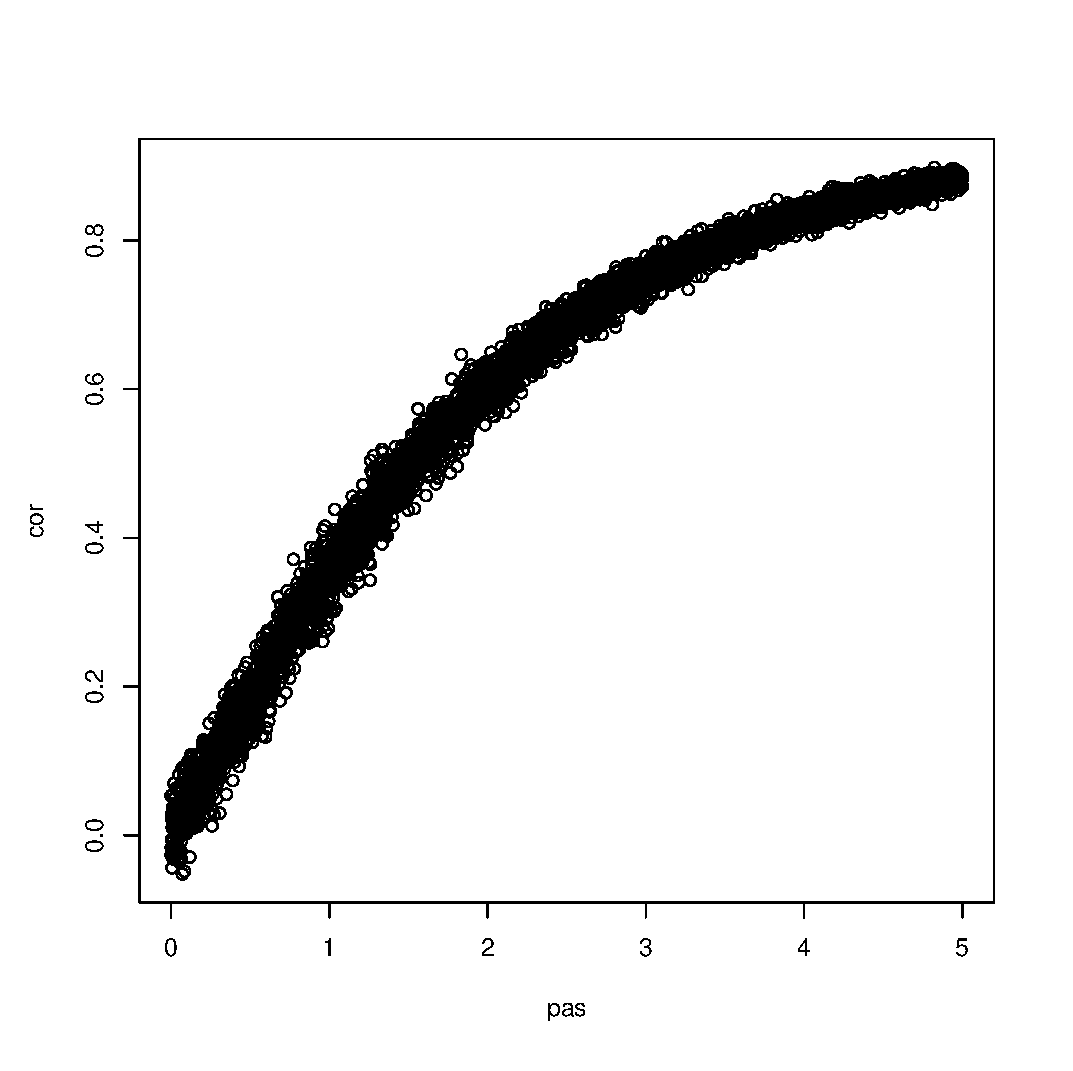
\includegraphics[width=6cm]{seriecascade.eps}}
\caption{   $\rho_{n,1}=f(\sigma_{1})$ }
\label{corrsigma1}
\end{figure}


\item En ajustant par tâtonnement:

Par exemple si on désire   diminuer la corrélation sur un chemin en série, on amincit progressivement le nuage  sur la régression globale en augmentant les $\sigma_{k}$ associés aux bruits des noeuds $X_{k}$ appartenant au chemin en série.

\end{itemize}


\item \textbf{ Structure série en cascade comprenant une V-structure:}

Focalisons nous  sur un triplet en V-structure :

$$X_{A}\longrightarrow X_{B}\longleftarrow X_{C}$$

La corrélation $\rho_{CA}$ en fonction de $\sigma_{A}$ pour une plage de valeurs $0\le \sigma_{A} \le 10$ est représenté ci-dessous:
\begin{figure}[H]
\centering
\fbox{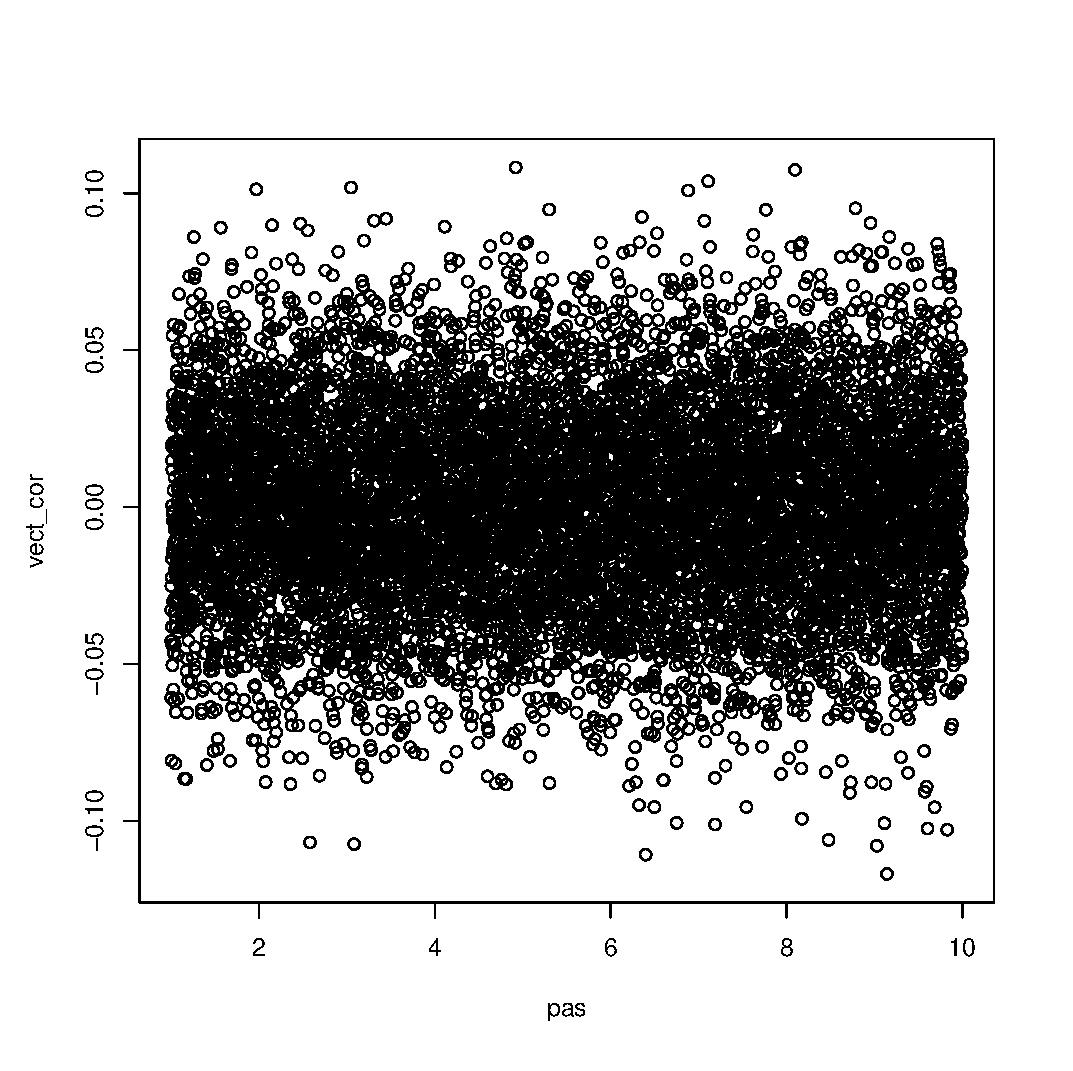
\includegraphics[width=6cm,height=5cm]{vstructabc.eps}}
\caption{   $\rho_{CA}=f(\sigma_{A})$ }
\end{figure}

Nous remarquons que $\rho_{CA}$ n'a pas de dépendance par rapport aux variations de $\sigma_{A}$, ceci n'est pas étonnant étant donné  que nous avons une V-structure.

En conséquence dans un cas général, si une chaîne allant de $A$ à $B$ sont les noeuds extrêmes d'une structure série  en cascade dans laquelle il y'a un ensemble de V-structures.

La modification de la corrélation $\rho_{AB}$ pourra se faire qu'à partir de la dernière V-structure croisée dans la chaîne $A-B$.

\item \textbf{Structure série en cascade comprenant une structure divergente:}

Considérons le triplet divergent  suivant:

$$X_{A}\longleftarrow X_{B}\longrightarrow X_{C}$$

La corrélation $\rho_{CA}$ en fonction de $\sigma_{A}$, pour $0\le \sigma_{A} \le 10$,   est donné  ci-dessous:

\begin{figure}[H]
\centering
\fbox{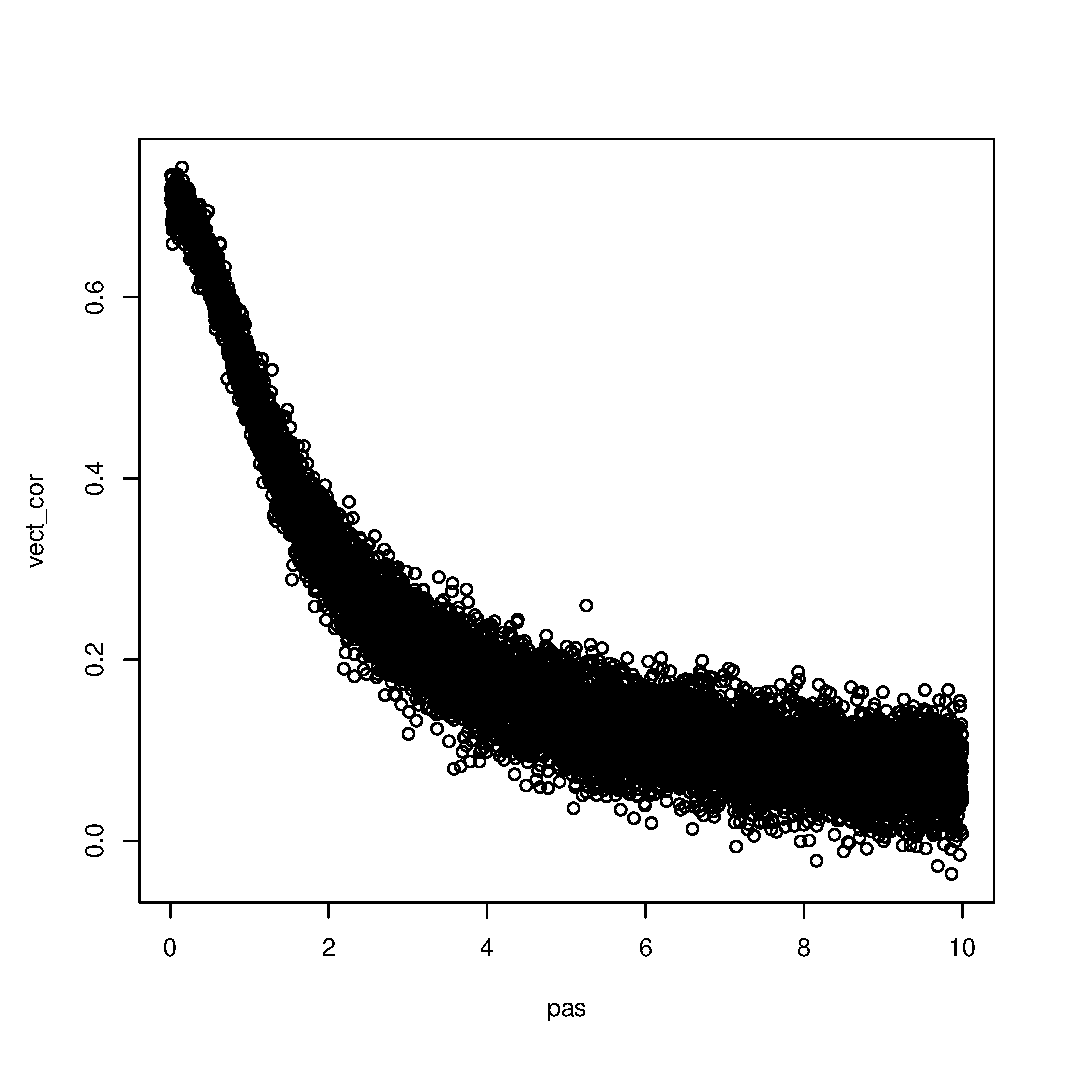
\includegraphics[width=6cm]{abc_divergent.eps}}
\caption{   $\rho_{CA}=f(\sigma_{A})$ }\label{fig:somefiglabel}
\end{figure}

Dans ce cas si la structure divergente se trouve au extrémité d'une chaîne, elle ne fera pas apparaître de V-structure et la corrélation diminuera dans la partie divergente pour ensuite augmenter dans la partie en série.

Si la structure divergente remplace un triplet en série  ailleurs qu'aux extrémités alors nous faisons apparaître une V-structure et on revient au cas précédent. 
\end{enumerate}














































































\newpage
\subsection{Création d'un jeux de données basé sur un jeux de données réaliste}
\label{jeux_data}
Nous allons partir ici d'une modélisation de dépendance et d'indépendance similaire à celui qui pourrait être établit pour le problème de l'achat de la voiture. Le modèle de dépendances et d'indépendances découlent des test statistiques qui ont été réalisé au préalable.
 
Si nous considérons cette modélisation, c'est pour la simple et bonne raison que nous allons en fin de section montrer le réalisme des valeurs générés en les comparant aux valeurs réalistes.

Supposons que nous avons à notre disposition uniquement le modèle de dépendance et d'indépendance suivant:

\[
\left\lbrace 
\begin{array}{lcl}
A \not\ci B \\
B \not\ci C\\
B \not\ci D\\
D \not\ci E\\
A\not\ci C \Longrightarrow A\ci C|B\\
A\not\ci D \Longrightarrow A\ci D|B \\
B \ci E \Longrightarrow B\not\ci E|D \\
C\not\ci D \Longrightarrow C\ci D|B\\
\end{array}\right.
\]

Les variables $(A,B,C,D,E)$ jouent le même rôle, respectivement, que les variables $(Cost,accel.,Pick.up,Braking.holding)$.


\subsubsection{Relation directes et graphe non-orienté}

La représentation des relations directes $A \not\ci B,\  B \not\ci C,\  B \not\ci D$ et $D \not\ci E$ nous donne le graphe non-orienté suivant:

\begin{figure}[H] 
    \center 
    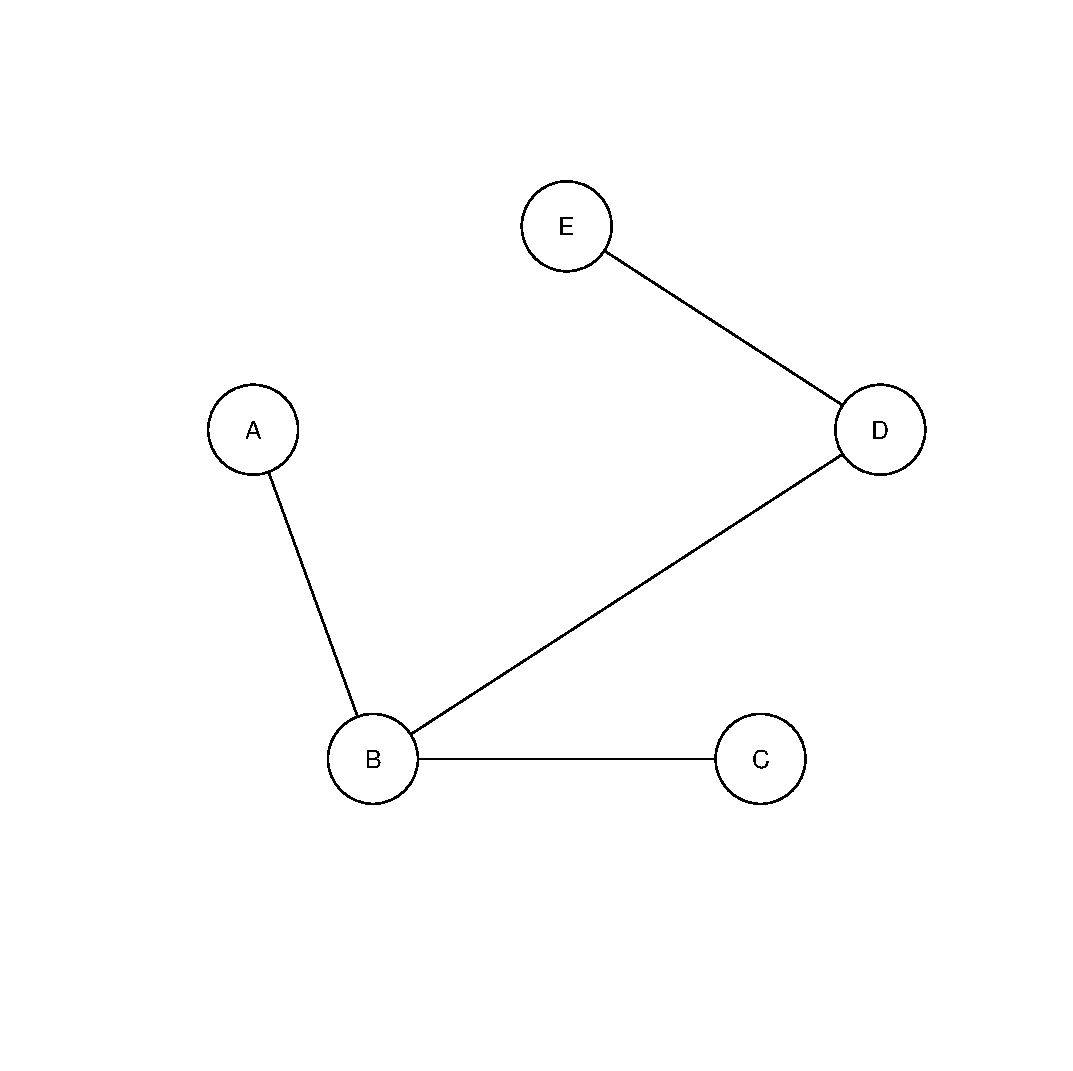
\includegraphics[width=6cm]{creatgraph.eps} 
    \caption{Représentation des relations directes.} 
\end{figure} 

\subsubsection{Relations indirectes et graphe orienté}
\begin{itemize}

\item La relation indirecte $B \ci E \Longrightarrow B\not\ci E|D$ impose que le triplet $(B,D,E)$ ne peut être qu'une V-structure.

\item La relation indirecte $A\not\ci C \Longrightarrow A\ci C|B$ impose que le triplet $(A,B,C)$ peut être \textbf{une} structure divergente ou \textbf{deux}  structure en série.

\item La relation indirecte $A\not\ci D \Longrightarrow A\ci D|B$ impose que le triplet $(A,B,D)$ peut être \textbf{une} structure divergente ou \textbf{une} structure en série.

\item La relation indirecte $C\not\ci D \Longrightarrow C\ci D|B$ implique que le triplet $(C,B,D)$ peut être  \textbf{une} structure divergente ou \textbf{une} structure en série.
\end{itemize}
Les  trois solutions vérifiant le modèle de dépendance et d'indépendance sont donc les suivantes:


\begin{figure}[H]
\centering
\subfigure[Solution n°1]{%
\fbox{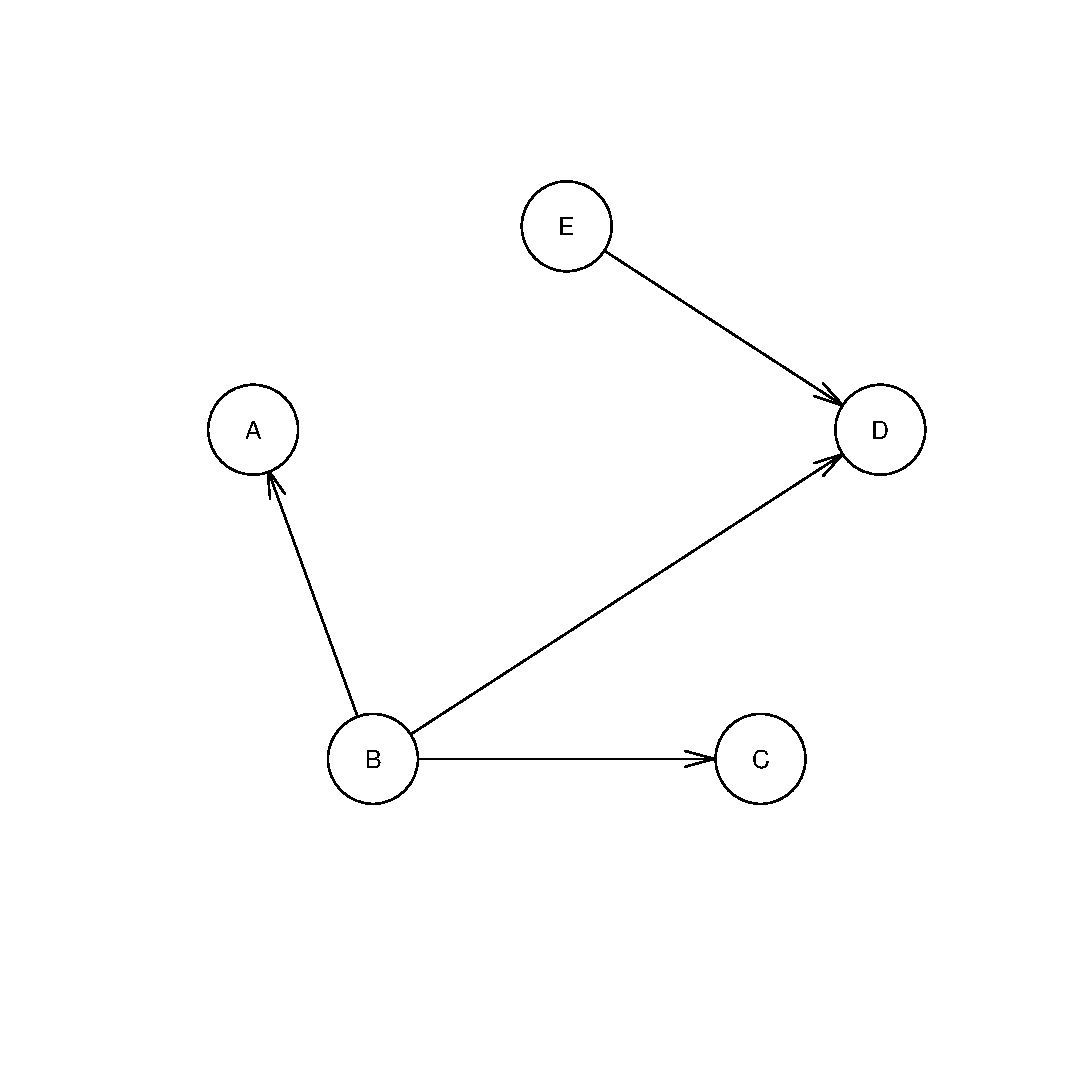
\includegraphics[width=0.4\textwidth]{sol1.eps}}%
  }
$\quad$
\subfigure[Solution n°2]{

 \fbox{ 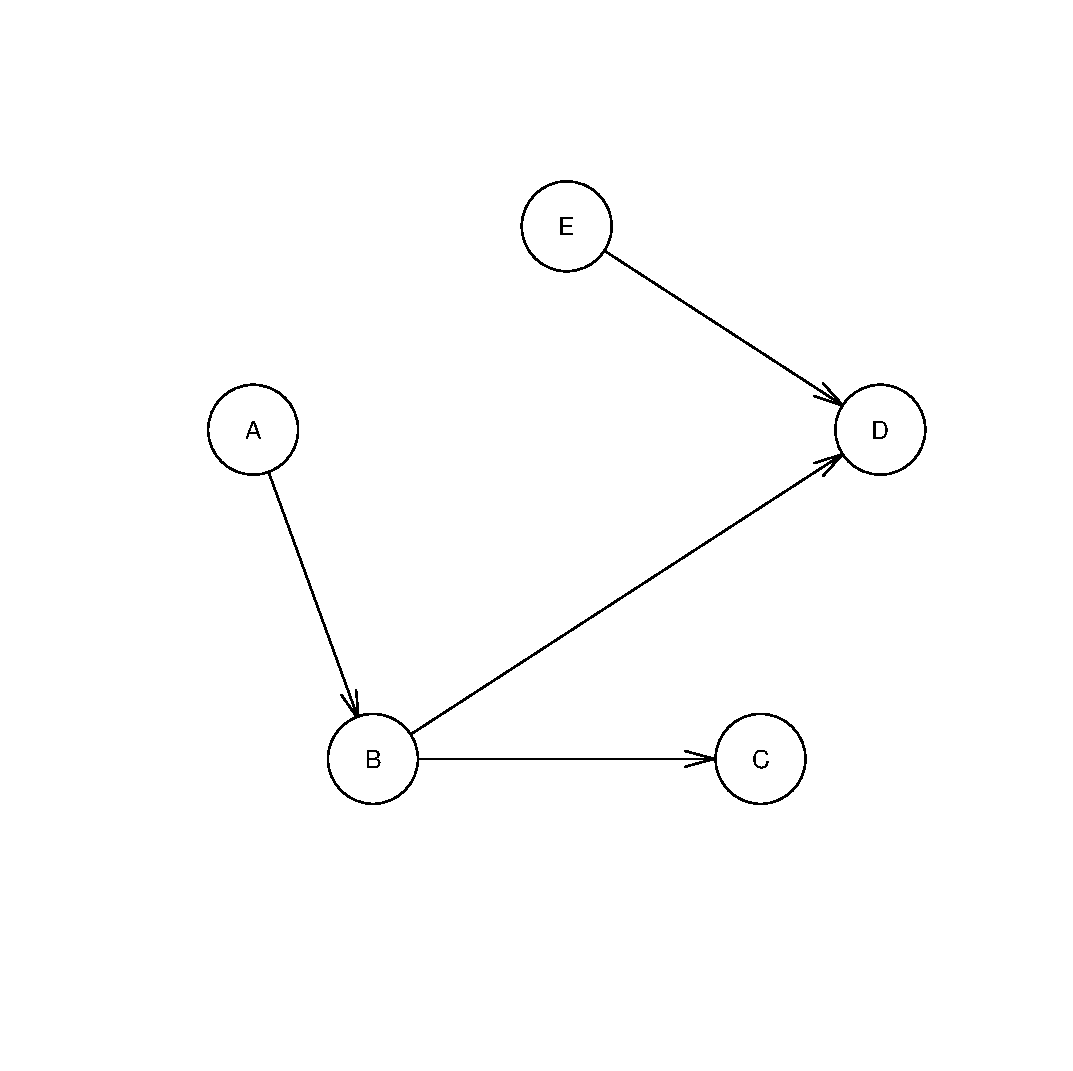
\includegraphics[width=0.4\textwidth]{sol2.eps}}%
}   
\\
\subfigure[Solution n°3]{

\fbox{ 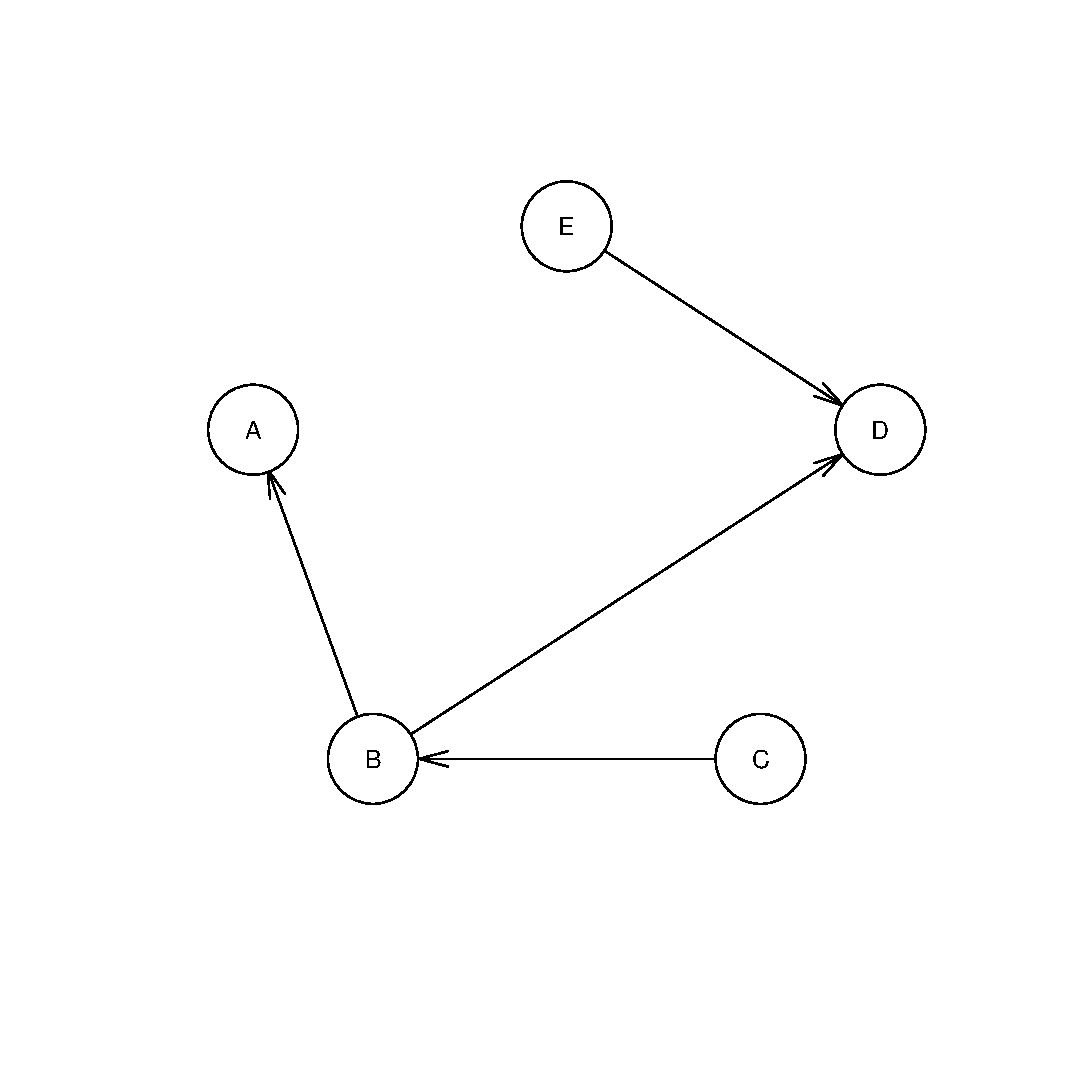
\includegraphics[width=0.4\textwidth]{sol3.eps}}%
 }

\end{figure}

La solution n°2 correspond au réseaux bayésien appris par la BIC-métrique(cf.Fig.\ref{bicmetric} )dans la section précédente, nous allons maintenant considérer cette solution pour générer nos valeurs.
Cette solution n °2 va nous permettre ultérieurement de valider le réalisme des données générés.




\subsubsection{Création du réseaux bayésien}

Une paramétrisation en $R$ à l'aide de la librairie "bnlearn" est décrite en annexe \ref{parametrisation}.

En utilisant les régressions associés au jeux de données de 14 alternatives, on obtient le système de paramétrisation suivant:


\begin{figure}[H]
\begin{center}
\begin{tabular}{|l|c|r|}
  \hline
Interception de la régression&Premier coefficient de régression&Deuxième coefficient régression  \\
  \hline
A\ \ 17229 &   &   \\ 
B\ \ 33.9289046 &-0.0002551&\\ 
C\ \ 6.085& 1.024 & \\ 
D\ \ 7.1364  &  -0.2048&0.4175  \\ 
E\ \ 2.232&0.5839544  & \\ 
\hline
\end{tabular}
\end{center}
\caption{Paramétrisation du réseaux}
\end{figure}
 
On fixe les écarts-types $\sigma$ intervenant dans les bruits $\eta(0,\sigma)$ comme étant  les écarts-types des vecteurs colonnes du jeux de données initial:

 $$\vec{S_{di}}\equiv (S_{dA}; S_{dB}; S_{dC}; S_{dD}; S_{dE})\equiv(2025.0149803  ;  0.8208402 ;   1.7847338;    0.3808695 ;   0.5839544)$$

Un échantillon de valeurs générés par le réseaux est  présenté en annexe \ref{creat_gener}


\newpage
\subsubsection{Validation des données générés}
La validation est faite en validant le modèle de dépendance et d'indépendance, une ACP et un diagramme en boîte.
\begin{enumerate}
\item \textbf{ Validation du modèle de dépendance et d'indépendance :}

Si le jeux de données générés est correcte, $\{A,B,C,D,E\}$ doit normalement vérifier le système suivant:
\[
\left\lbrace 
\begin{array}{lcl}
A \not\ci B \\
B \not\ci C\\
B \not\ci D\\
D \not\ci E\\
A\not\ci C \Longrightarrow A\ci C|B\\
A\not\ci D \Longrightarrow A\ci D|B \\
B \ci E \Longrightarrow B\not\ci E|D \\
C\not\ci D \Longrightarrow C\ci D|B\\
\end{array}\right.
\]


Le jeux de données générés vérifient bien statistiquement le modèle de dépendance et d'indépendance:


\begin{figure}[H]
\begin{center}
\begin{tabular}{|l|c|r|}
  \hline
  Relation & Corrélation & P-value \\
  \hline
  
\hline \hline \\
$A\cap B$&-0.54&$<2.2.10^{-16}$\\
$B\cap C$&0.5175&$<2.2.10^{-16}$\\
$B\cap D$&-0.4135&$<2.2.10^{-16}$\\
$D\cap E$&0.4749&$<2.2.10^{-16}$\\
 \hline \hline 
$A\cap C$&-0.2743&$<2.2.10^{-16}$\\
$A\cap C|B$&0.0071&0.8215\\
 \hline \hline 
$A\cap D$&0.2112&$1.512.10^{-11}$\\
$A\cap D|B$&-0.0158 &0.6188\\
 \hline \hline 
$B\cap E$&0.023&0.4675\\
$B\cap E|D$&0.2738&$<2.2.10^{-16}$\\
 \hline \hline 
$C\cap D$&-0.26&$2.2.10^{-16}$\\
$C\cap D|B$&-0.0591&0.16184\\

\hline
\end{tabular}
\end{center}
\caption{Test statistiques pour 1000 valeurs }
\end{figure}

\newpage

\item \textbf{Validation du réalisme des données générés}

Notre de jeux de données créée possède le centre de gravité $\vec{G}$ (moyenne) et le vecteur écart-type suivant:
\[
\left\lbrace 
\begin{array}{lcl} 
\vec{G}\equiv(17277.017601;    29.521423;    36.372200;     2.014466;     2.237097)\\ \\
\vec{S_{d}}\equiv (1991.5736216;    0.9752285;    2.0801198;    0.4997543;    0.5645750)\\ 
\end{array}\right.
\]

On constate une bonne proximité des moyennes et des écarts-types.


Les valeurs propres , les vecteurs propres normées obtenus à partir d'une ACP normée  sont les suivants:

\[
\left\lbrace 
\begin{array}{lcl} 
\lambda_{1}=2.3632170 && \vec{x_{1}}\equiv (0.4860036; -0.5414876; -0.2875029;  0.52139093;  0.3407128)\\
\lambda_{2}=1.1966196 && \vec{x_{2}}\equiv( 0.2884098; -0.3004653; -0.4497740; -0.37415732; -0.6958808)\\
\lambda_{3}=0.8221576 && \vec{x_{3}}\equiv ( 0.5069560; -0.1835779;  0.8156589; -0.08946249; -0.1897153)\\
\lambda_{4}=0.3277016 &&\vec{x_{4}}\equiv (0.4624732;  0.2399957; -0.1766391; -0.63421732;  0.5432197)\\
\lambda_{5}=0.2903041 &&\vec{x_{5}}\equiv ( -0.4579677; -0.7247158;  0.1361791; -0.42180879;  0.2618877)\\
\end{array}\right.
\]
Nous avons la qualité d'information en 3D suivante:
$$\delta=\frac{(\lambda_{1}+\lambda_{2}+\lambda_{3})}{(\lambda_{1}+\lambda_{2}+\lambda_{3}+\lambda_{4}+\lambda_{5})}=0.8763989$$

La projection des individus dans le sous-espace munis du repère ($\vec{G},\vec{x_{1}},\vec{x_{2}},\vec{x_{3}}$) est donnée ci-dessous :


\begin{figure}[H]
\centering
\fbox{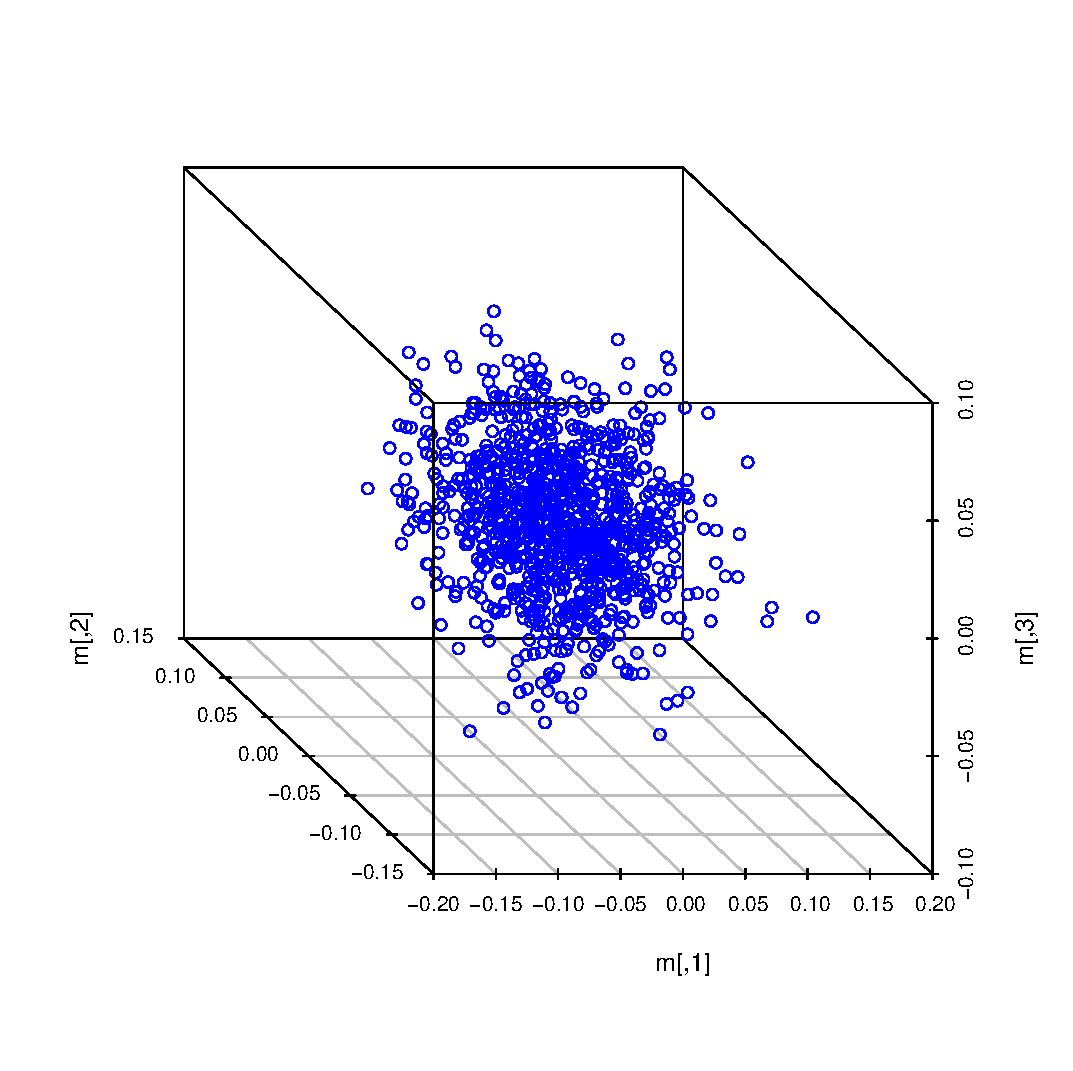
\includegraphics[width=8cm]{cubecreat.eps}}
\caption{Projection du nuage de points sur sous-espace munis du repère ($\vec{G},\vec{x_{1}},\vec{x_{2}},\vec{x_{3}}$)}\label{fig:somefiglabel}
\end{figure}
\newpage
En projetant les nuages de points associés aux deux jeux  sur les plans principaux : 

\begin{figure}[H]
\fbox{\includegraphics[width=5cm]{proj12data.eps}}\hfill
\fbox{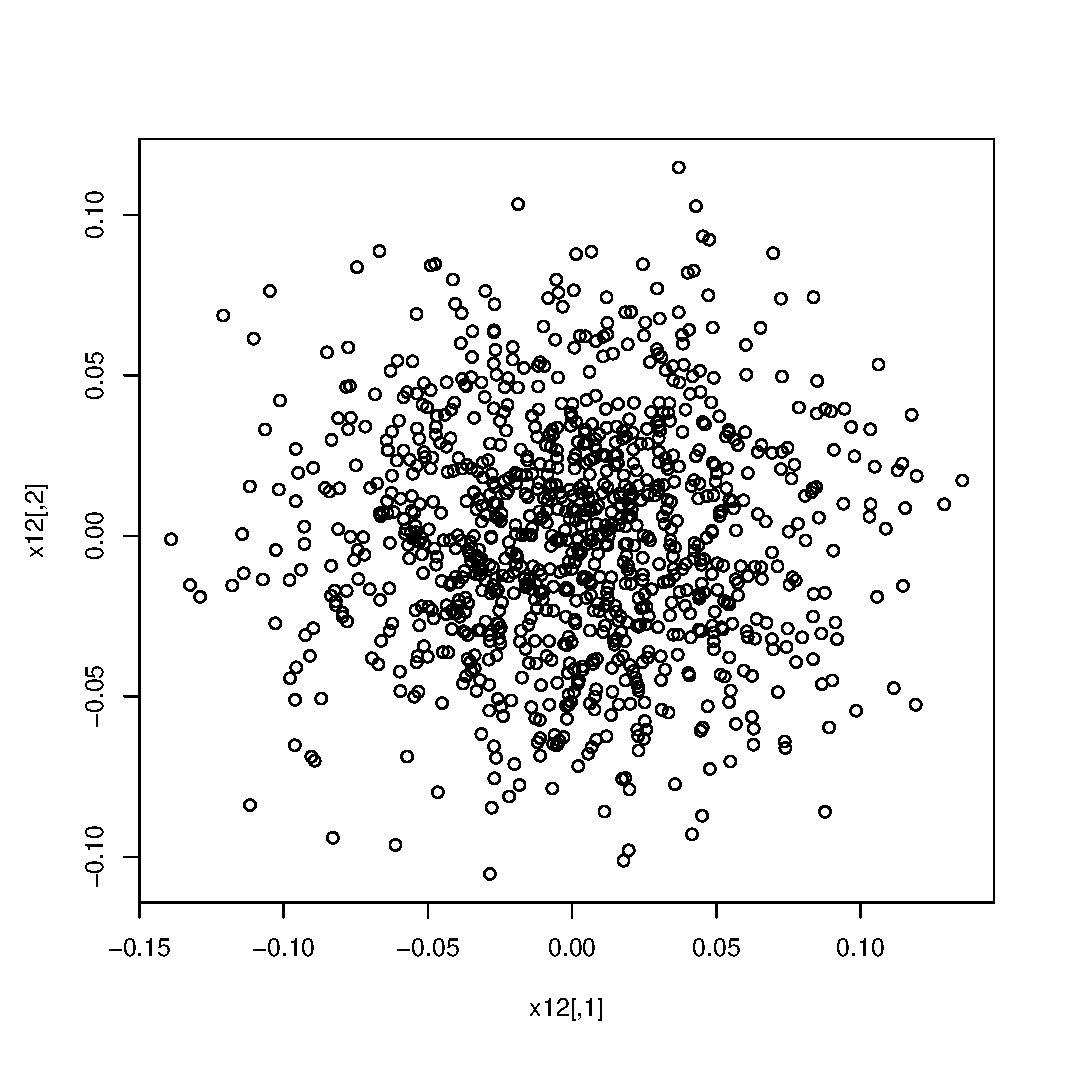
\includegraphics[width=5cm]{projcreat12.eps}}
\caption{Projection du nuage de points sur le plan ($\vec{G},\vec{x_{1}},\vec{x_{2}}$)}\label{fig:somefiglabel}
\end{figure}


\begin{figure}[H]
\fbox{\includegraphics[width=5cm]{proj13data.eps}}\hfill
\fbox{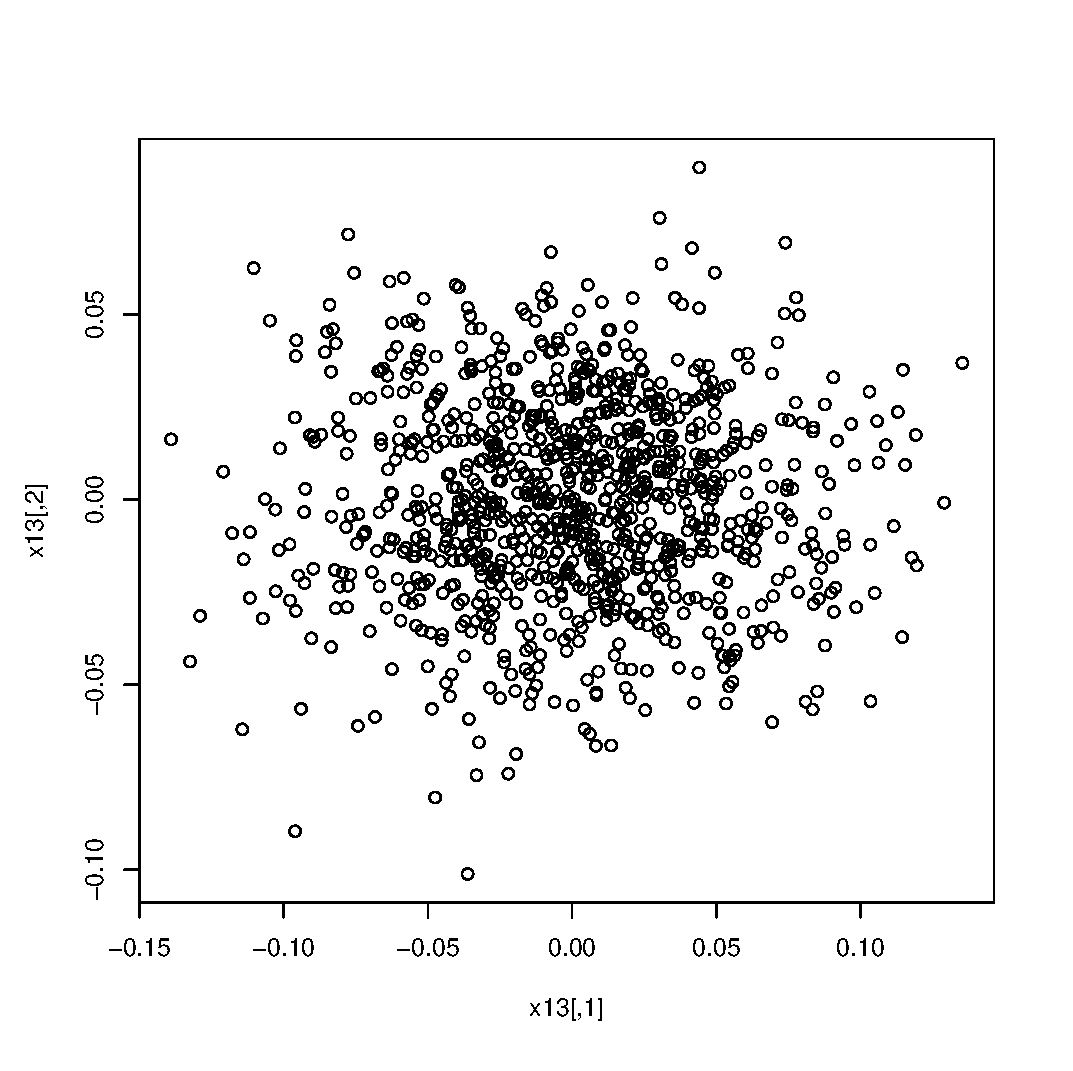
\includegraphics[width=5cm]{projcreat13.eps}}
\caption{Projection du nuage de points sur le plan ($\vec{G},\vec{x_{1}},\vec{x_{3}}$) }\label{fig:somefiglabel}
\end{figure}



\begin{figure}[H]
\fbox{\includegraphics[width=5cm]{proj23data.eps}}\hfill
\fbox{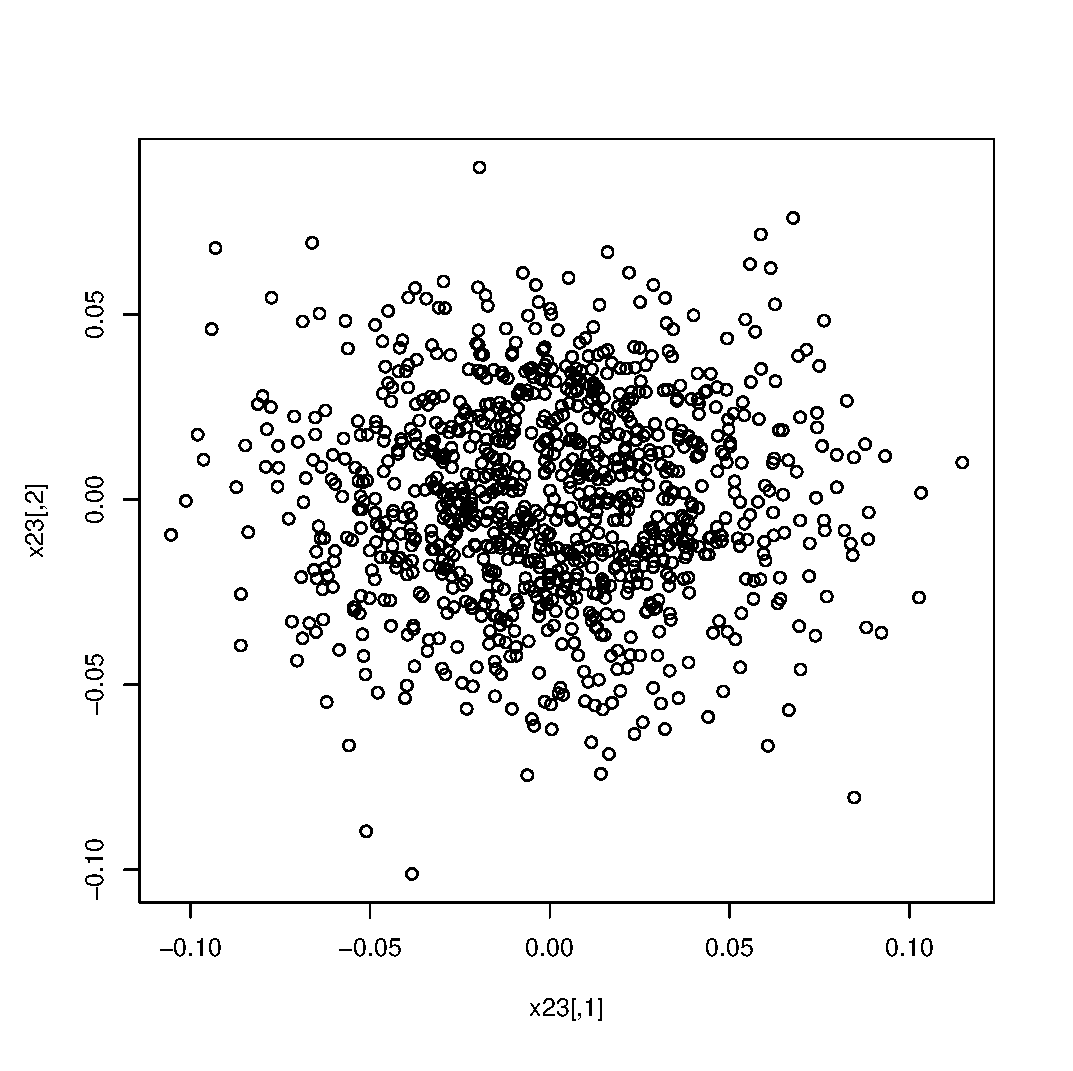
\includegraphics[width=5cm]{projcreat23.eps}}
\caption{Projection du nuage de points sur le plan ($\vec{G},\vec{x_{2}},\vec{x_{3}}$) }\label{fig:somefiglabel}
\end{figure}

\end{enumerate}















































































\newpage
\begin{appendices}
\section{Programmes du faible et du grand bruitages} 
\label{programme}
\begin{figure}[H] 
    \center 
   \includegraphics[scale=1.4,height=20cm]{ajoutb.eps} 
    \caption{Code en R du faible et du grand bruitages} 
\end{figure} 

\newpage

\section{Apprentissage: Implantation d'une usine de traitement de déchet}

\label{apprentissage_usine}
Le problème consiste à optimiser le meilleure emplacement d'une usine.

les critères intervenants dans le choix de l'emplacement sont repris dans le tableaux ci-dessous:
\begin{figure}[H] 
    \center 
    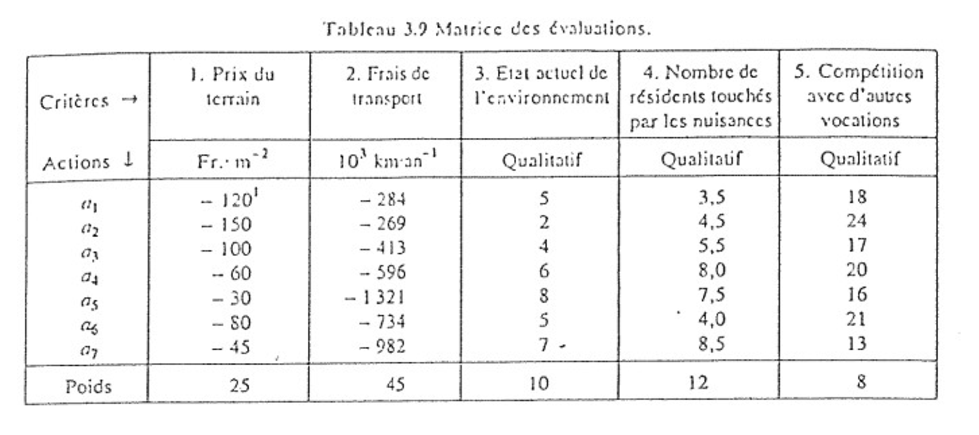
\includegraphics[width=10cm,height=5cm]{CasMaystr.eps} 
    \caption{Jeux de données} 
\end{figure} 


\subsubsection{Utilisation de la BIC-métrique}
En appliquant la BIC-métrique sur notre jeux de données:

\begin{figure}[H] 
    \center
    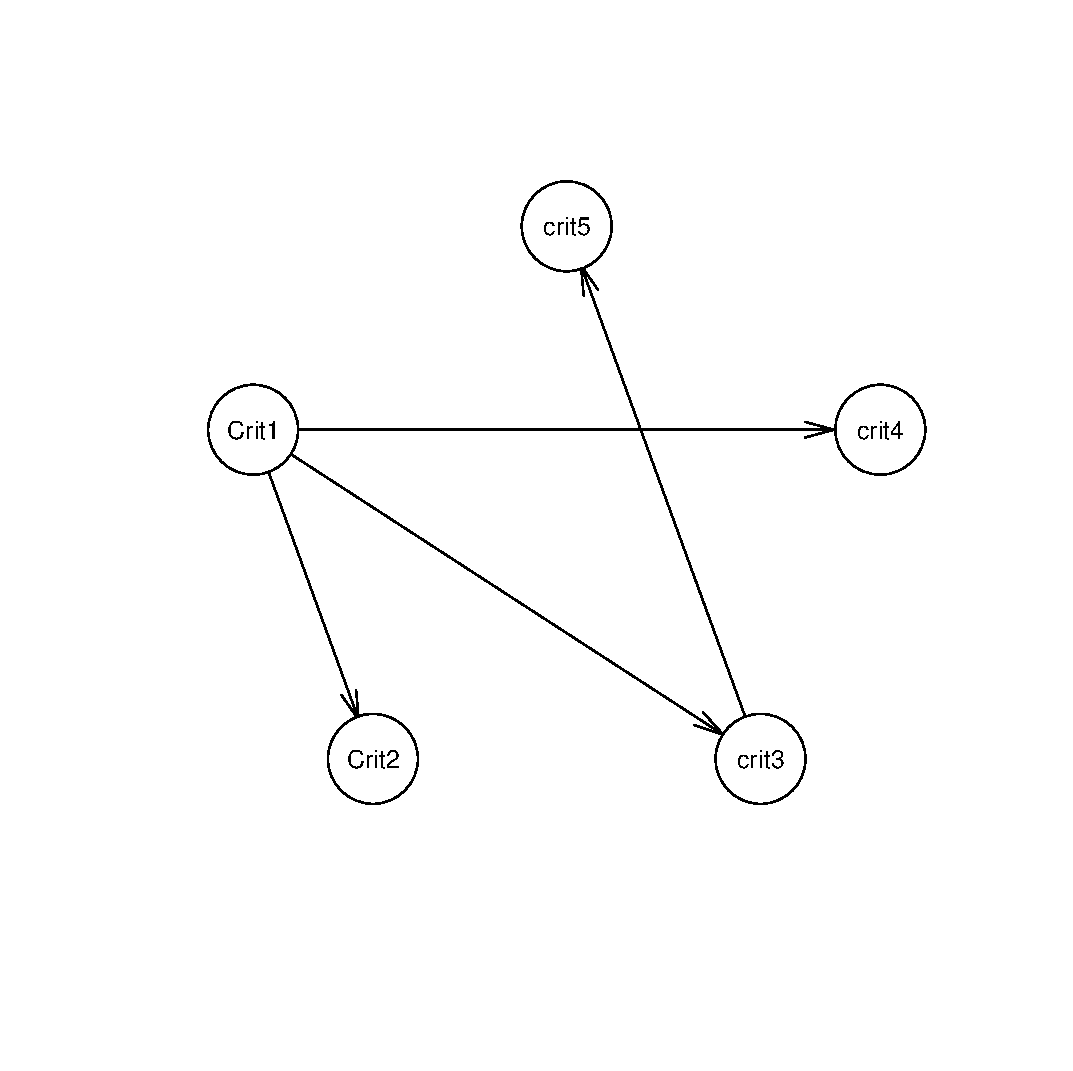
\includegraphics[width=5cm]{grapheterrain.eps} 
    \caption{Réseaux obtenu avec l'utilisation de la BIC-métrique} 
\end{figure} 
\newpage
En effectuant des test statistiques sur le jeux de données des 7 valeurs initiales  et du jeux de données obtenus par génération de 1000 valeurs:
\begin{center}
\begin{tabular}{|l|c|r|}
  \hline
  Relation & Corrélation & P-value \\
  \hline
   $Crit2 \cap  Crit3$& 0.8661& $<$=0.01171  \\
      $ Crit2 \cap Crit3 | Crit1$       & 0.075                    & = 0.8877   \\
 \hline
\hline
$Crit1  \cap  Crit5$ &     0.6772    & $<$0.09468 \\
$Crit1  \cap  Crit5|Crit3$ &     -0.1197  & = 0.8212\\
\hline \hline

$Crit2  \cap  Crit5$ & -0.5875 &  $<$ 0.1654 \\
$Crit2  \cap  Crit5|Crit1$ & 0.0879& =0.8684\\
$Crit2 \cap Crit5 |Crit3$ &   0.1778& =0.736 \\
\hline
\end{tabular}
\end{center}


\begin{figure}[H]
\begin{center}
\begin{tabular}{|l|c|r|}
  \hline
  Relation & Corrélation & P-value \\
  \hline
   $Crit2 \cap  Crit3$& 0.8541& $<$2.2e-16  \\
      $ Crit2 \cap Crit3 | Crit1$       & -0.0184                      & = 0.5614   \\
 \hline
\hline
$Crit1  \cap  Crit5$ &     0.6976    & $<$2.2e-16 \\
$Crit1  \cap  Crit5|Crit3$ &     -0.0072   & = 0.819 \\
\hline \hline

$Crit2  \cap  Crit5$ & -0.6228 &  $<$ 2.2e-16 \\
$Crit2  \cap  Crit5|Crit1$ & 0.0347& =0.2727\\
$Crit2 \cap Crit5 |Crit3$ &   0.0015& =0.9614 \\
\hline
\end{tabular}
\end{center}
\caption{Test statistiques pour 1000 valeurs }
\end{figure}
\textbf{Commentaires}:
\begin{itemize}
\item Le triplet $(Crit2,Crit1,Crit3)$ a une structure divergente et nous avons bien une dégradation de la corrélation par le conditionnement de $Crit1$.

\item Le triplet $(Crit1,Crit3,Crit5)$ a une structure en série et la dégradation de la corrélation est aussi visible par conditionnement de $Crit3$.

\item Pour ce qui en est du chemin reliant le $Crit2$ au $Crit5$,nous voyons que les deux sous-structures à l'interstice de $Crit2$ et $Crit5$ se comportent comme des sous-structures divergente et en  série.{\\}

\end{itemize}
\newpage
\subsubsection{BGE métrique}
Nous allons, comme pour l'exemple des voitures, comparer les deux métriques:

\begin{figure}[H] 
    \center 
    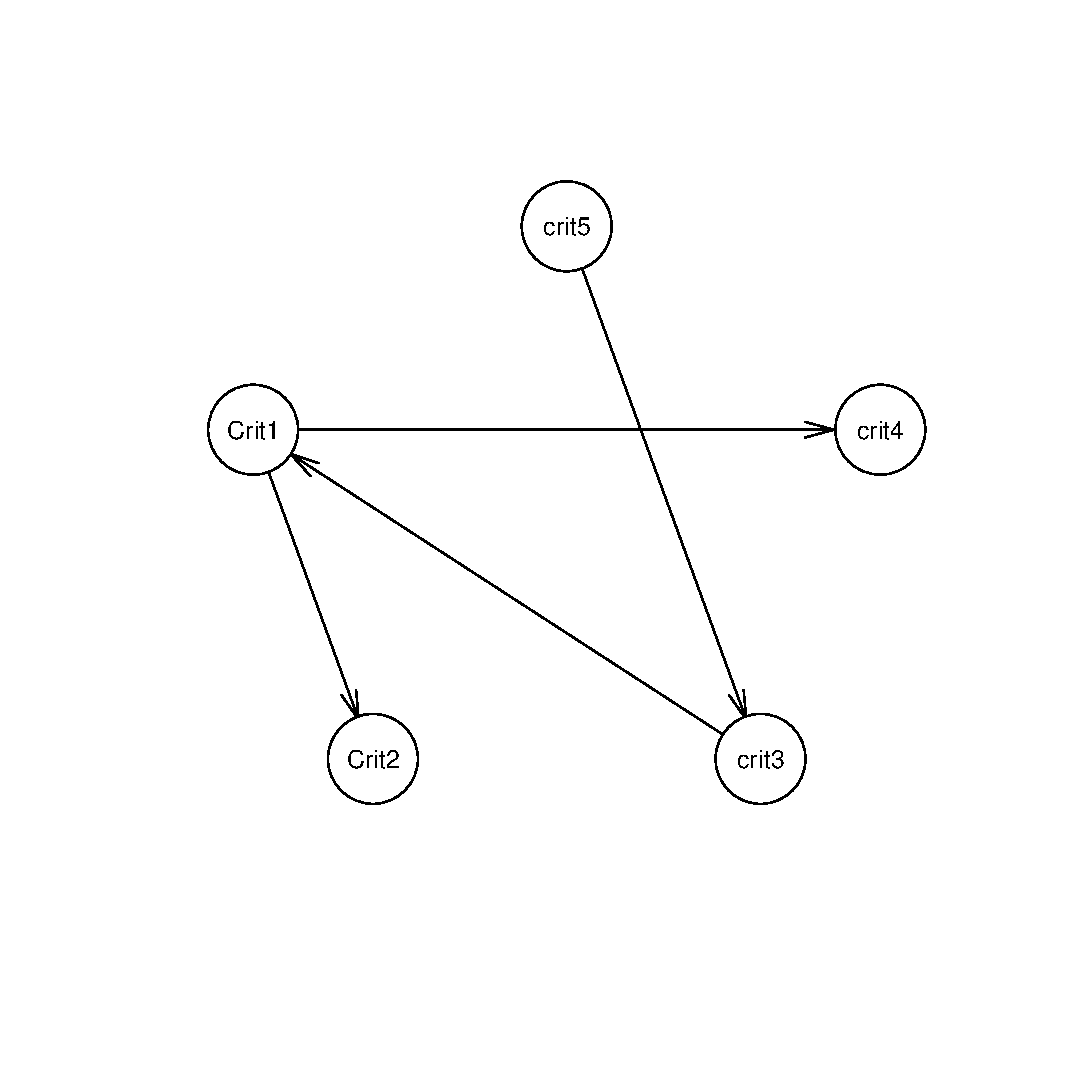
\includegraphics[width=5cm]{tabubge.eps} 
    \caption{Tabu avec BGE-metric} 
\end{figure} 

Les deux réseaux $RB_1 \equiv RB_2$ sont équivalents, par conséquent ils vérifient les mêmes relations de dépendances et d'indépendances.Les commentaires statistiques seront alors similaires à ceux qui ont été fait pour la BIC-métrique.


\subsubsection{Normalisation, ACP 2D et tableaux des corrélations}
Le tableaux normalisé, la matrice des corrélations ainsi que l'ACP 2D sont donné par:

\begin{figure}[H]
\begin{tabular}{llllll}
  \hline
Altérnatives&  Crit1& Crit2 & Crit3&Crit4&Crit5 \\
  \hline
1& 0.20512821 &0.06175255 &0.13513514 &0.08433735 &0.1395349\\
2 &0.25641026 &0.05849098 &0.05405405 &0.10843373 &0.1860465\\
3 &0.17094017 &0.08980213 &0.10810811 &0.13253012 &0.1317829\\
4 &0.10256410 &0.12959339 &0.16216216 &0.19277108 &0.1550388\\
5 &0.05128205 &0.28723636 &0.21621622 &0.18072289 &0.1240310\\
6 &0.13675214 &0.15959991 &0.13513514 &0.09638554 &0.1627907\\
7 &0.07692308 &0.21352468 &0.18918919 &0.20481928 &0.1007752\\

\hline

\end{tabular}
\caption{Jeux de données normalisés}
\end{figure}



\begin{figure}[H]
\begin{tabular}{llllll}
  \hline
                &  Crit1& Crit2 & Crit3&Crit4&Crit5 \\
  \hline
Crit1  &1.0000000 &-0.9076551 &-0.9426532 &-0.7916770  &0.6771882\\
Crit2 &-0.9076551  &1.0000000  &0.8661152  &0.6632595 &-0.5874959\\
Crit3 &-0.9426532  &0.8661152  &1.0000000  &0.6847494 &-0.7465923\\
Crit4 &-0.7916770  &0.6632595  &0.6847494  &1.0000000 &-0.5825127\\
Crit5  &0.6771882 &-0.5874959 &-0.7465923 &-0.5825127 & 1.0000000\\
\hline

\end{tabular}
\caption{Tableaux des corrélations}
\end{figure}


\begin{figure}[H] 
    \center 
    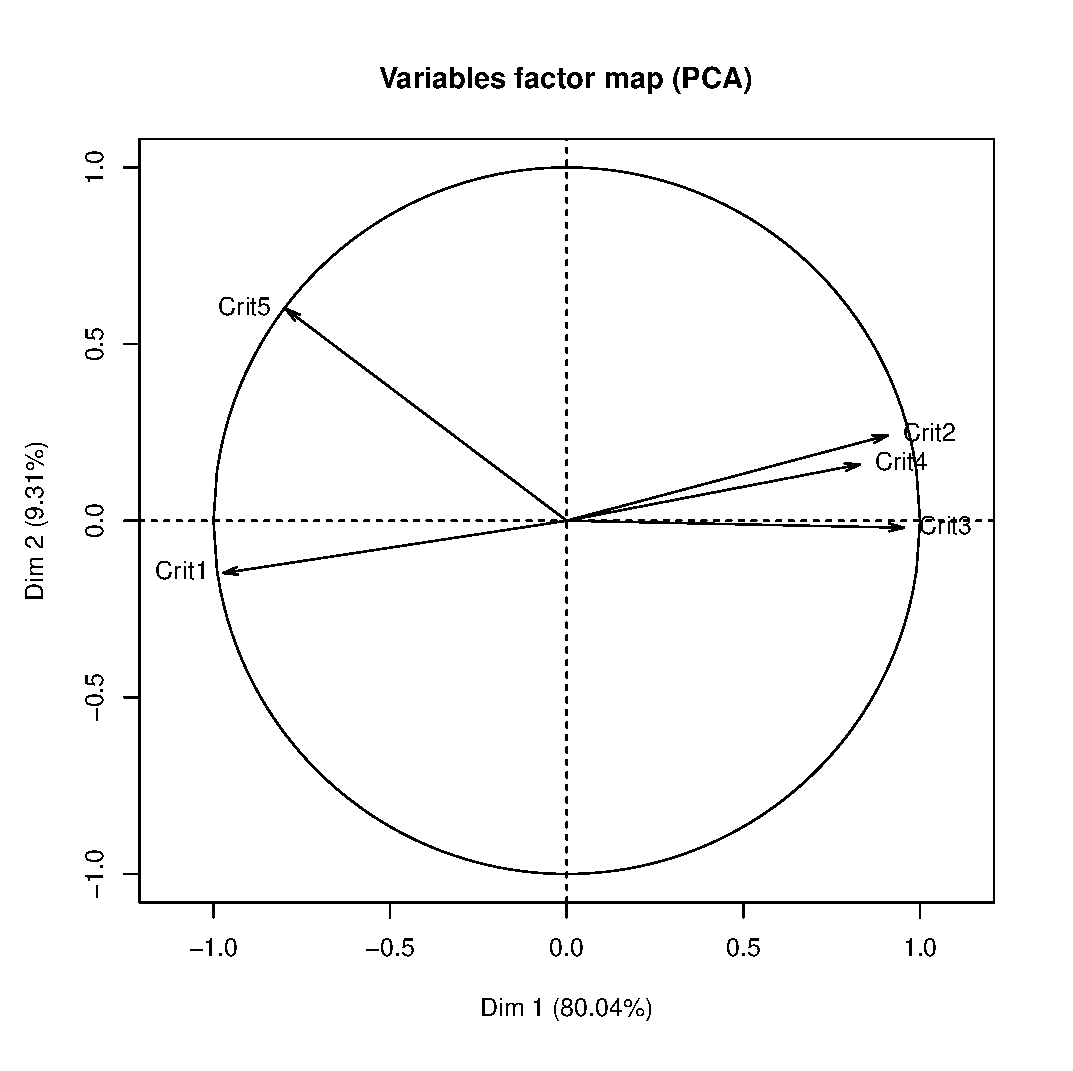
\includegraphics[width=8cm]{ACP_TERRAIN.eps} 
    \caption{Représentation ACP 2D} 
\end{figure} 




\subsubsection{Atténuation de la corrélation par grand bruitage du jeux de donné}

Nous allons profiter de cette exemple pour montrer que la méthode des grands bruitages permet de décorréller de manière significative pair à pair toutes  les variables d'un jeux de donnée. Mais cette exemple montrera clairement que la méthode est laborieuse.

Si nous observons l'ACP 2D et la matrice des corrélation du jeux original, nous constatons que les critères $Crit2,Crit3, Crit4$ sont trop corrélée.

Nous allons donc ,dans un premier temps, appliquer un bruitage de  $Crit2/Crit4.$

Après l'application d'un ajout de grand bruit, on obtient le tableaux de données Fig. \ref{tab3}, la matrice des corrélations Fig.\ref{matcorr3} et l'ACP 2D Fig.\ref{acp3} suivantes:

\begin{figure}[H]
\begin{tabular}{llllll}
  \hline
Altérnatives&  Crit1& Crit2 & Crit3&Crit4&Crit5 \\
  \hline
1 &0.20512821 &0.002545604 &0.13513514 &0.08433735& 0.1395349\\
2 &0.25641026 &0.447382979 &0.05405405 &0.10843373 &0.1860465\\
3 &0.17094017 &0.081289041 &0.10810811 &0.13253012 &0.1317829\\
4 &0.10256410 &0.197642822 &0.16216216 &0.19277108 &0.1550388\\
5 &0.05128205 &0.210222506 &0.21621622 &0.18072289 &0.1240310\\
6 &0.13675214 &0.050491568 &0.13513514 &0.09638554 &0.1627907\\
7 &0.07692308 &0.010425481 &0.18918919 &0.20481928 &0.1007752\\

\hline

\end{tabular}
\caption{Jeux de données normalisé après un fort bruitage.Paramètre=(data,2,4,0.2,100,500)}
\label{tab3}
\end{figure}



\begin{figure}[H]
\begin{tabular}{llllll}
  \hline
                &  Crit1& Crit2 & Crit3&Crit4&Crit5 \\
  \hline
Crit1  &1.0000000  &0.361784641 &-0.9426532 &-0.791677016 & 0.6771882\\
Crit2  &0.3617846  &1.000000000 &-0.4590201 &-0.005636093  &0.6589878\\
Crit3 &-0.9426532 &-0.459020058  &1.0000000 & 0.684749378 &-0.7465923\\
Crit4 &-0.7916770 &-0.005636093  &0.6847494  &1.000000000 &-0.5825127\\
Crit5  &0.6771882  &0.658987764 &-0.7465923 &-0.582512704  &1.0000000\\
\hline

\end{tabular}
\caption{Tableaux des corrélations après bruitage}
\label{matcorr3}
\end{figure}


\begin{figure}[H] 
    \center 
    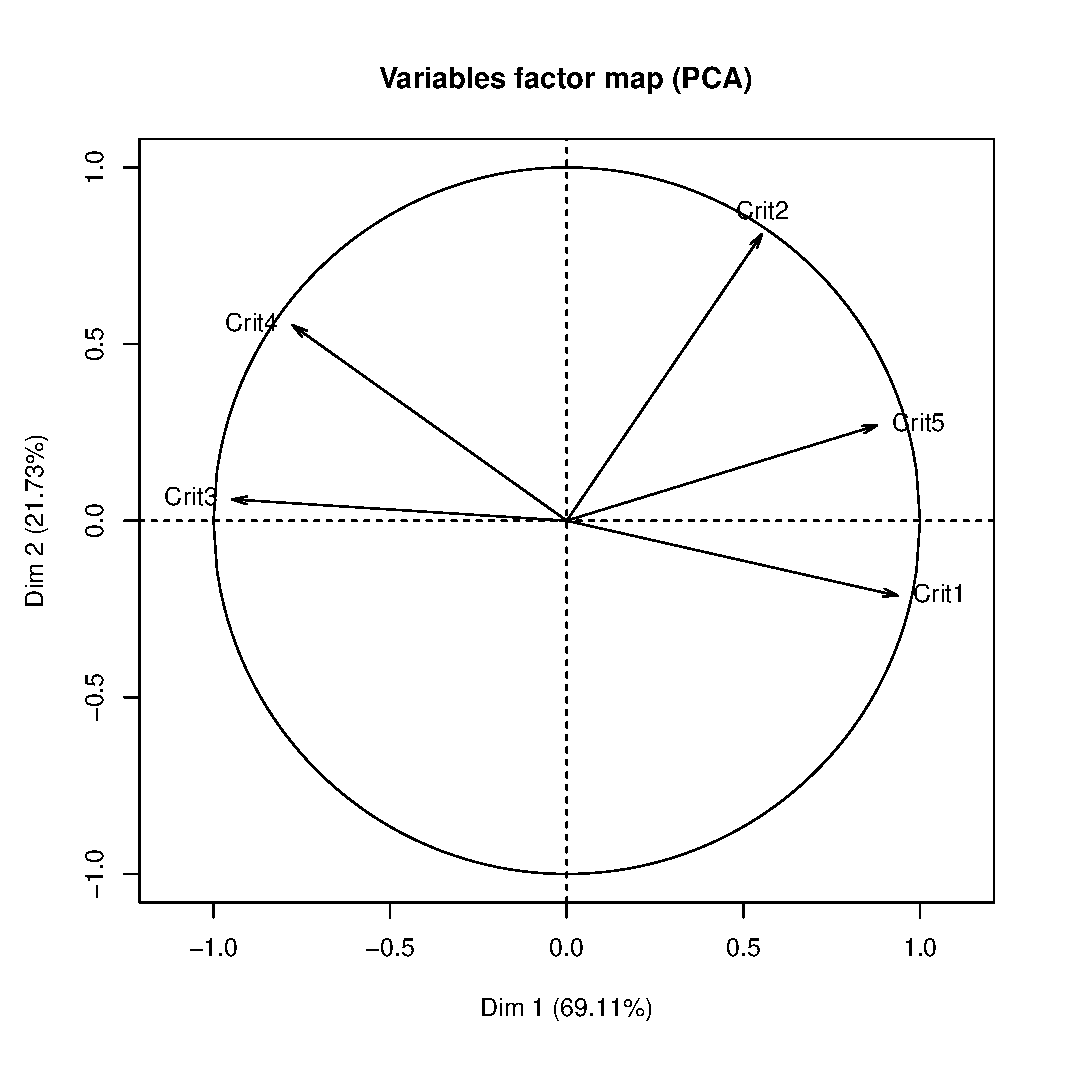
\includegraphics[width=8cm]{ACP_TERRIAN_BRUIT_FORT1.eps} 
    \caption{Représentation ACP 2D après bruitage} 
\label{acp3}
\end{figure} 

Si nous supposons que la corrélation entre $ Crit3$ et $Crit1$ est trop importante, nous pouvons à nouveaux appliquer la méthode pour un bruitage sur $Crit3$ par rapport au Crit1. On obtient alors les nouvelles  caractéristiques suivantes:

\begin{figure}[H]
\begin{tabular}{llllll}
  \hline
Altérnatives&  Crit1& Crit2 & Crit3&Crit4&Crit5 \\
  \hline
1 &0.20512821 &0.002545604 &0.11821624 &0.08433735 &0.1395349\\
2 &0.25641026 &0.447382979 &0.12152874 &0.10843373 &0.1860465\\
3 &0.17094017 &0.081289041 &0.03196543 &0.13253012 &0.1317829\\
4 &0.10256410 &0.197642822 &0.05129533 &0.19277108 &0.1550388\\
5 &0.05128205 &0.210222506 &0.14957736 &0.18072289 &0.1240310\\
6 &0.13675214 &0.050491568 &0.22386537 &0.09638554 &0.1627907\\
7 &0.07692308 &0.010425481 &0.30355154 &0.20481928 &0.1007752\\
\hline
\end{tabular}
\caption{Jeux de donné normalisé après un fort bruitage.Paramètre=(Newdata,3,1,0.5,100,500)}
\end{figure}
\begin{figure}[H]
\begin{tabular}{llllll}
  \hline
                &  Crit1& Crit2 & Crit3&Crit4&Crit5 \\
  \hline
Crit1  &1.0000000  &0.361784641 &-0.3625993 &-0.791677016  &0.6771882\\
Crit2  &0.3617846  &1.000000000 &-0.3278609 &-0.005636093  &0.6589878\\
Crit3 &-0.3625993 &-0.327860915  &1.0000000  &0.184573938 &-0.3772684\\
Crit4 &-0.7916770 &-0.005636093  &0.1845739  &1.000000000 &-0.5825127\\
Crit5  &0.6771882  &0.658987764 &-0.3772684 &-0.582512704  &1.0000000\\
\hline

\end{tabular}
\caption{Tableaux des corrélations après bruitage}
\end{figure}

\begin{figure}[H] 
    \center 
    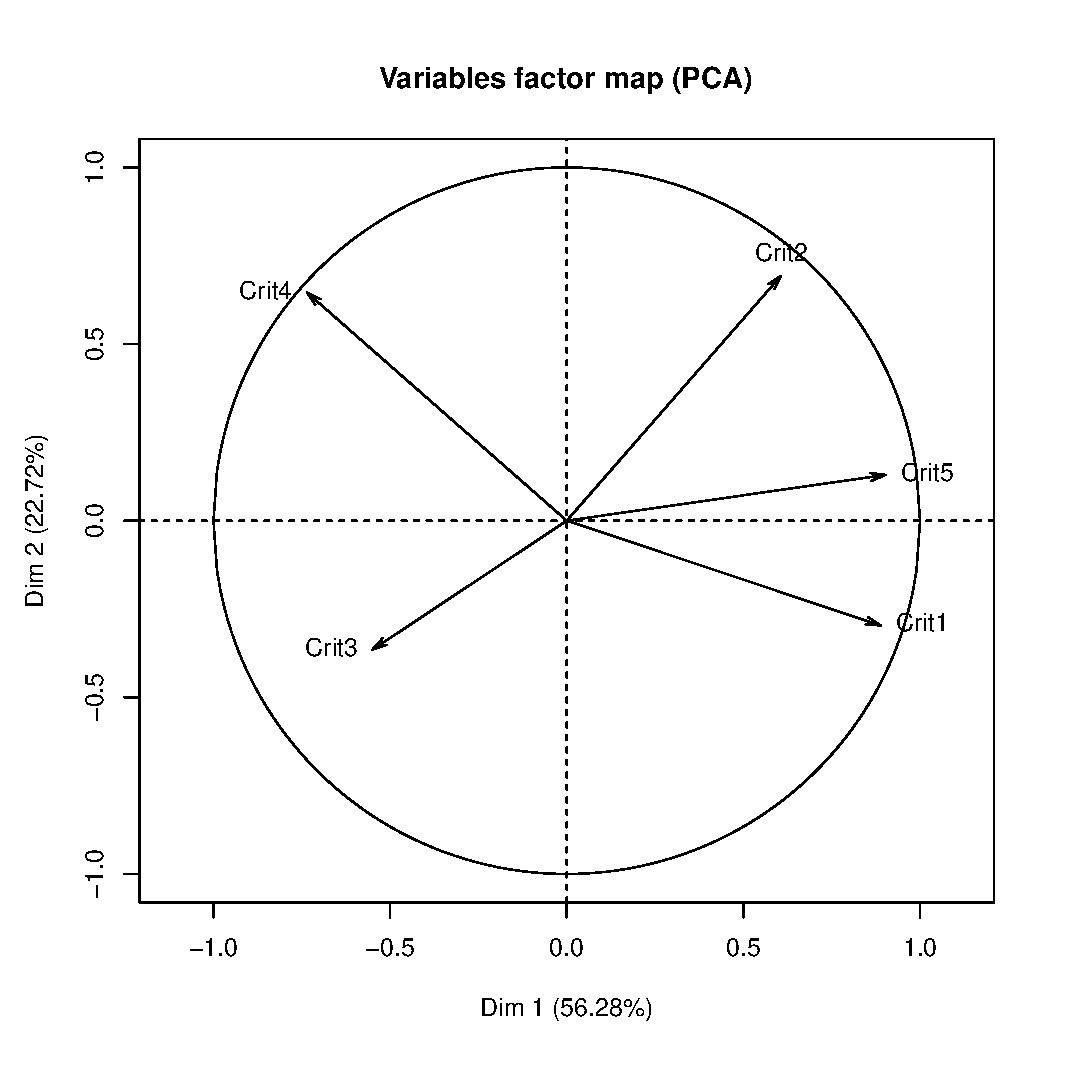
\includegraphics[width=8cm]{ACP_BRUIT_FORT_TERRAIN2.eps} 
    \caption{Représentaion ACP 2D après bruitage} 
\end{figure} 
Comme nous l'avons dit en début de section, nous allons décorrélée  pas à pas les variables paire à paire.

Nous n'allons pas expliciter toutes les itérations mais après avoir utilisé les atténuations suivantes  :


Crit4/Crit1,Crit5/Crit1,Crit2/Crit1,Crit3/Crit5 et Crit1/Crit3:

Nous obtenons le jeux de données Fig. \ref{tab4} la matrice des corrélations Fig. \ref{matcorr4} suivantes:

\begin{figure}[H]
\begin{tabular}{llllll}
  \hline
                &  Crit1& Crit2 & Crit3&Crit4&Crit5 \\
  \hline
Crit1  &1.0000000 & 0.29119647 &-0.28055311 & 0.1671216 &-0.40527303\\
Crit2  &0.2911965  &1.00000000  &0.01534193 -&0.4399796 &-0.08815628\\
Crit3 &-0.2805531  &0.01534193  &1.00000000  &0.2558913 &-0.15816836\\
Crit4 & 0.1671216 &-0.43997961  &0.25589131  &1.0000000 &-0.28114772\\
Crit5 &-0.4052730 &-0.08815628 &-0.15816836 &-0.2811477 & 1.00000000\\
\hline

\end{tabular}
\caption{Tableaux des corrélations final}
\label{tab4}
\end{figure}

\begin{figure}[H]
\begin{tabular}{llllll}
  \hline
Altérnatives&  Crit1& Crit2 & Crit3&Crit4&Crit5 \\
  \hline
1 &0.15918958 &0.005101735& -0.05358094 &0.19585608 &0.20447272\\
2 &0.40808353 &0.228050314 &-0.06069470 &0.15734412 &0.04501011 \\
3 &0.05032273 &0.190639028 &-0.08847885 &0.01636222 &0.34171059\\
4 &0.08568759 &0.159997582  &0.47117538 &0.20860008 &0.25576037\\
5 &0.04599601 &0.124336727  &0.08085311 &0.20474925 &0.05224913\\
6 &0.10103185 &0.169206291  &0.21747420 &0.08657656 &0.04289240\\
7 &0.14968871 &0.122668323  &0.43325178 &0.13051168 &0.05790469\\
\hline
\end{tabular}
\caption{Jeux de données normalisé final}
\label{matcorr4}
\end{figure}
\subsubsection{Validation des valeurs générés}

La qualité d'information $\delta$ d'une ACP 3D appliquée au jeux de 1000 donnée  est exprimé ci-dessous:

$$\delta=\frac{(\lambda_{1}+\lambda_{2}+\lambda_{3})}{(\lambda_{1}+\lambda_{2}+\lambda_{3}+\lambda_{4}+\lambda_{5})}=0.9665694$$

L'ACP 3D donne:

\begin{figure}[H]
\fbox{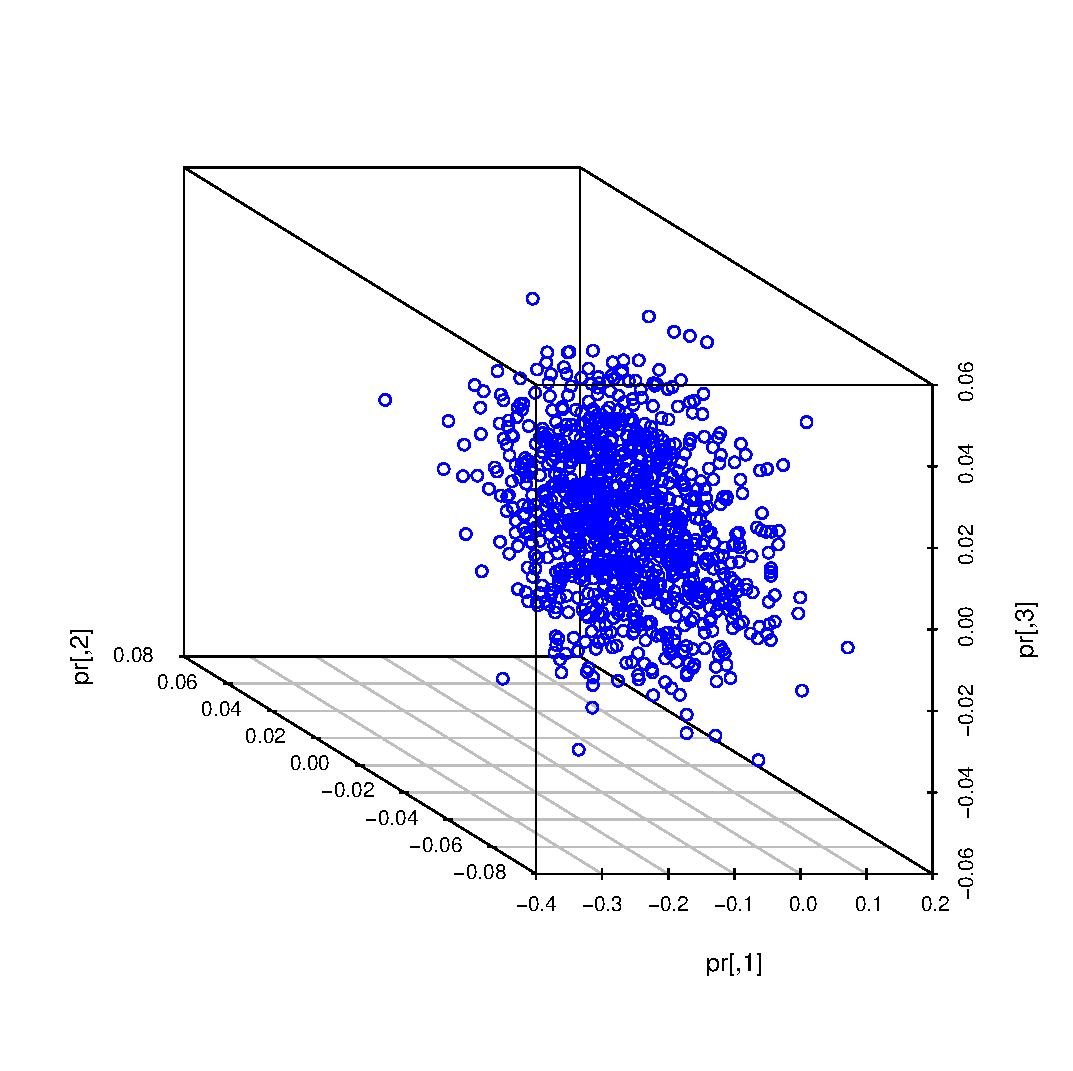
\includegraphics[width=6cm]{cubedataex1.eps}}\hfill
\fbox{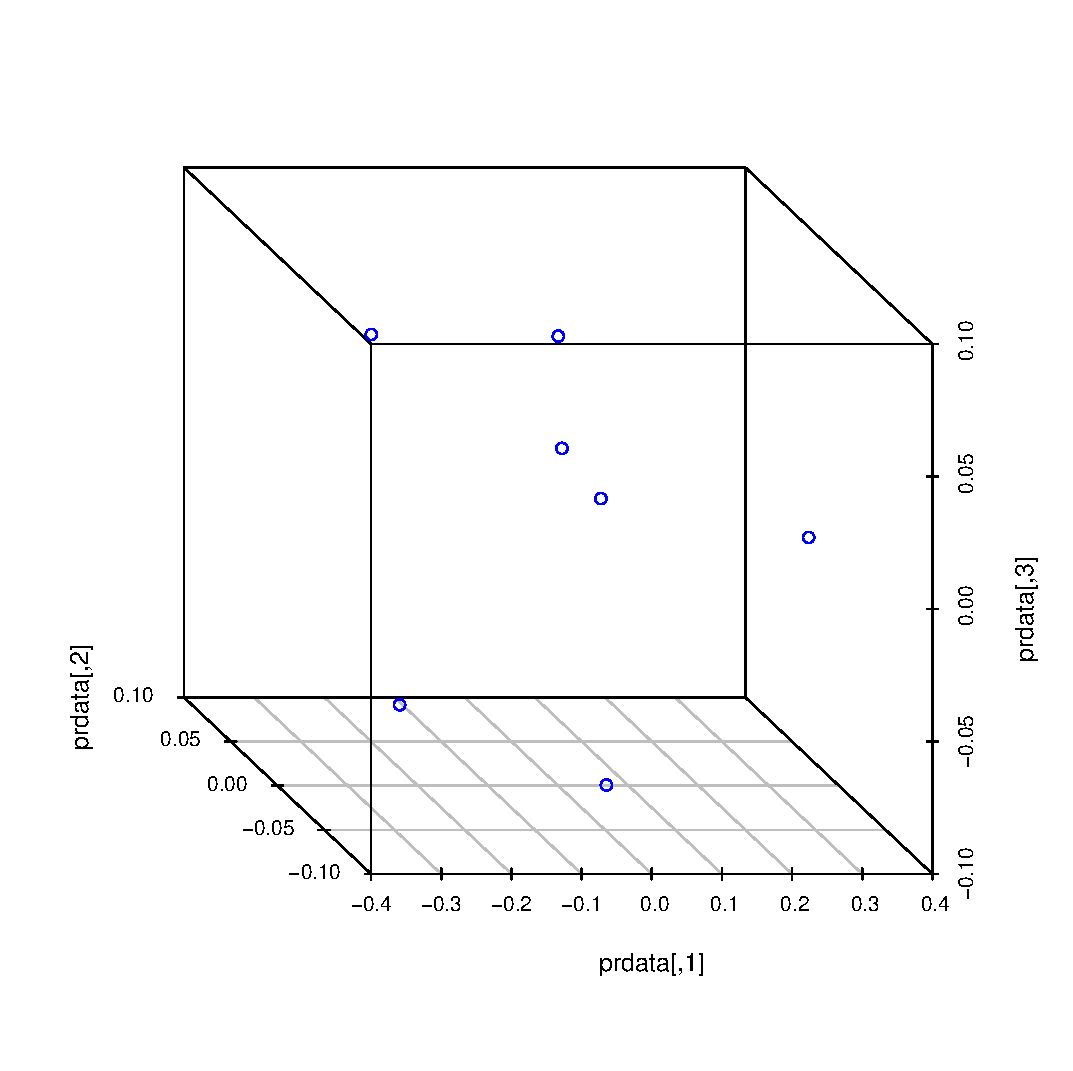
\includegraphics[width=6cm]{cubegenerex1.eps}}
\caption{Projection du jeux de données initial et du jeux de 1000 valeurs sur le sous-espace munis du repère $(\vec{G},\vec{x_{1}},\vec{x_{2}},\vec{x_{3}})$}\label{fig:somefiglabel}
\end{figure}


Afin de mieux voir la proximité des individus, nous projetons le nuage de points sur les plans principaux (voir Fig.\ref{planprincip1}, Fig.\ref{planprincip2} et    Fig.\ref{planprincip3}    )      :
\begin{figure}[H]
\includegraphics[width=6cm]{projdataex12.eps}\hfill
\includegraphics[width=6cm]{projgenerex12.eps}
\caption{Projection du jeux de données initial et du jeux de 1000 valeurs sur le plan $(\vec{G},\vec{x_{1}},\vec{x_{2}})$}
 \label{planprincip1}  
\end{figure}
\begin{figure}[H]
\includegraphics[width=6cm]{projgenerex13.eps}\hfill
\includegraphics[width=6cm]{projdataex13.eps}
\caption{Projection du jeux de données initial et du jeux de 1000 valeurs sur le plan $(\vec{G},\vec{x_{1}},\vec{x_{3}})$}
 \label{planprincip2}  
\end{figure}
\begin{figure}[H]
\includegraphics[width=6cm]{projdataex23.eps}\hfill
\includegraphics[width=6cm]{projgenerex23.eps}
\caption{Projection du jeux de données initial et du jeux de 1000 valeurs sur le plan $(\vec{G},\vec{x_{2}},\vec{x_{3}})$}
 \label{planprincip3}  
\end{figure}

On obtient pour l'ensemble des points, dans les 5 dimensions, le diagramme en boîte suivant:

\begin{figure}[H]
\fbox{\includegraphics[width=6cm]{boxdataex1.eps}}\hfill
\fbox{\includegraphics[width=6cm]{boxgenerex1.eps}}
\caption{Diagramme en boîte pour le jeux initial (gauche) et le jeux obtenu après avoir généré1000 valeurs }\label{fig:somefiglabel}
\end{figure}





\newpage

\section{Apprentissage: Achat d'une guitare}

\label{apprentissage_guitare}
Le tableaux ci-dessous est un tableaux normalisé provenant d'un jeux de données reprenant différentes guitares comme alternatives et différents critères.
\begin{figure}[H]
\begin{tabular}{llllll}
  \hline
Altérnatives&  Crit1& Crit2 & Crit3&Crit4&Crit5 \\
  \hline
1  &0.08715403 &0.09661836 &0.11627907 &0.10416667 &0.09615385\\
2  &0.11912173 &0.09661836 &0.11627907 &0.10416667 &0.07692308\\
3  &0.10726003 &0.09420290 &0.11627907 &0.10416667 &0.09615385\\
4  &0.08547152 &0.09661836 &0.06976744 &0.08333333 &0.09615385\\
5  &0.08406943 &0.09661836 &0.06976744 &0.08333333 &0.09615385\\
6  &0.10650290 &0.08212560 &0.06976744 &0.08333333 &0.09615385\\
7  &0.09865119 &0.08695652 &0.09302326 &0.10416667 &0.09615385\\
8  &0.09248198 &0.08212560 &0.11627907 &0.10416667 &0.09615385\\
9  &0.08917305 &0.08695652 &0.11627907 &0.10416667 &0.09615385\\
10 &0.06286980 &0.09420290 0&.04651163 &0.06250000 &0.07692308\\
11 &0.06724433 &0.08695652 &0.06976744 &0.06250000 &0.07692308\\
\hline
\end{tabular}
\caption{Jeux de données normalisé }
\end{figure}
 $\left\lbrace 
\begin{array}{lcl}
\text{Crit1=Prix.}\\
\text{Crit2=Audiofanzine}.\\
\text{Crit3=Notoriété}.\\
\text{Crit4=Son}.\\
\text{Crit5=Manche}.\\
\text{Crit6=Forme}.\\
\end{array}\right.${\\}

\subsubsection{Application de la BIC-metric}
\begin{figure}[H] 
    \center 
    \includegraphics[width=5cm]{IM_GRAPHE_GUIT.eps} 
    \caption{Tabu avec BGE-metric } 
\end{figure} 
\begin{figure}[H]
\begin{center}
\begin{tabular}{|l|c|r|}
  \hline
  Relation & Corrélation & P-value \\
  \hline
$Crit1 \cap Crit5$&0.3001&$=0.3699 $\\
$Crit1 \cap Crit5 | Crit4$&-0.1928&0.5935 \\
$Crit5 \cap Crit3$&0.3255&0.3287 \\
$Crit5 \cap Crit3 |Crit4$&-0.5149&$=0.1278$\\
$Crit1 \cap Crit3$&0.6148&$0.0441$\\
$Crit1 \cap Crit3 |Crit4$&  -0.2031&$=0.5736$\\
\hline
\end{tabular}
\end{center}
\caption{Test statistique pour les 11 alternatives }
\end{figure}





\begin{figure}[H]
\begin{center}
\begin{tabular}{|l|c|r|}
  \hline
  Relation & Corrélation & P-value \\
  \hline
$Crit1 \cap Crit5$&0.2772&$<2.2.10^{-16} $\\
$Crit1 \cap Crit5 | Crit4$&0.0521&0.09963 \\
$Crit5 \cap Crit3$&0.0312&0.324 \\
$Crit5 \cap Crit3 |Crit4$&-0.6205&$<2.2.10^{-16}$\\
$Crit1 \cap Crit3$&0.6428&$<2.2.10^{-16} $\\
$Crit1 \cap Crit3 |Crit4$&  0.0187&$<0.5541$\\
\hline
\end{tabular}
\end{center}
\caption{Test statistiques pour 1000 valeurs }
\end{figure}
\textbf{Commentaires:}

\begin{itemize}
\item Le triplet $(Crit1,Crit4,Crit5)$  est une structure en série, ce qui implique que le conditionnement de $Crit4$ diminue la corrélation.
\item Le triplet $(Crit5,Crit4,Crit3)$ est une V-structure , ce qui implique la diminution de la corrélation par conditionnement de $Crit4$.
\item Le triplet $(Crit1,Crit4,Crit3)$ est aussi une structure en série , nous sommes donc bien dans la même situation que le premier exemple.

\end{itemize}


\subsubsection{Application de la BGE-métrique}
\begin{figure}[H] 
    \center 
    \includegraphics[width=5cm]{GUITARE_GRAPHE_BGE.eps} 
    \caption{Application de la BGE-métrique } 
\end{figure} 

Regardons ce qu'il se passe  du point de vue statistique pour notre jeux de départ:

\begin{figure}[H]
\begin{center}
\begin{tabular}{|l|c|r|}
  \hline
  Relation & Corrélation & P-value \\
  \hline
$Crit1 \cap Crit5$&0.3001&$=0.3699 $\\
$Crit1 \cap Crit5 | Crit4$&-0.1928&0.5935 \\
$Crit5 \cap Crit3$&0.3255&0.3287 \\
$Crit5 \cap Crit3 |Crit4$&-0.5149&$=0.1278$\\
$Crit1 \cap Crit3$&0.6148&$0.0441$\\
$Crit1 \cap Crit3 |Crit4$&  -0.2031&$=0.5736$\\
\hline
\end{tabular}
\end{center}
\caption{Test statistiques pour les 11 alternatives }
\end{figure}

Le triplet $(Crit1,Crit4,Crit5)$ joue bien le rôle d'une V-structure. De plus il n'y pas de corrélation entre $Crit5$ et $Crit3$ car la P-value est de  0.3287.

La BIC-métrique, nous donne encore le réseaux le plus vraisemblable.

\subsubsection{Validation des données du jeux générés}

La qualité d'information $\delta$ de l'ACP 3D appliquée au jeux de 1000 données générés vaut  :

$$\delta=\frac{(\lambda_{1}+\lambda_{2}+\lambda_{3})}{(\lambda_{1}+\lambda_{2}+\lambda_{3}+\lambda_{4}+\lambda_{5})}=0.9070546$$

Projection dans le sous-espace munis du repère $(\vec{G},\vec{x_{1}},\vec{x_{2}},\vec{x_{3}})$ :

 \begin{figure}[H]
\fbox{\includegraphics[width=6cm]{cubeex3.eps}}\hfill
\fbox{\includegraphics[width=6cm]{cubeex3g.eps}}
\caption{Projection du jeux de données initial et du jeux de 1000 valeurs sur sous-espace munis du repère $(\vec{G},\vec{x_{1}},\vec{x_{2}},\vec{x_{3}})$}\label{fig:somefiglabel}
\end{figure}

Les projections du jeux initial et du jeux de données générés sur les plans principaux sont les suivantes:

\begin{figure}[H]
\includegraphics[width=6cm]{prdata12ex3.eps}\hfill
\includegraphics[width=6cm]{prgener12ex3.eps}
\caption{Projection du jeux de données initial et du jeux de 1000 valeurs sur le plan $(\vec{G},\vec{x_{1}},\vec{x_{2}})$}\label{fig:somefiglabel}
\end{figure}


\begin{figure}[H]
\includegraphics[width=6cm]{prdata13ex3.eps}\hfill
\includegraphics[width=6cm]{prgener13ex3.eps}
\caption{Projection du jeux de données initial et du jeux de 1000 valeurs sur le plan $(\vec{G},\vec{x_{1}},\vec{x_{3}})$}\label{fig:somefiglabel}
\end{figure}

\begin{figure}[H]
\includegraphics[width=6cm]{prdata23ex3.eps}\hfill
\includegraphics[width=6cm]{prgener23ex3.eps}
\caption{Projection du jeux de données initial et du jeux de 1000 valeurs sur le plan $(\vec{G},\vec{x_{2}},\vec{x_{3}})$}\label{fig:somefiglabel}
\end{figure}

 \begin{figure}[H] 
    \center 
   \fbox{ \includegraphics[width=5cm]{boitedifin.eps} }
    \caption{Diagramme en boîte } 
\label{newboxplot}
\end{figure} 







































\newpage
\section{Paramétrisation d'un réseaux  en $R$ avec l'utilisation de la librairie "bnlearn"}
\label{parametrisation}
Nous présentons ici la manière dont rentre les paramètres d'un réseaux en  $R$

Pour le réseaux décrits ci-dessous:

\begin{figure}[H] 
    \center 
    \includegraphics[width=5cm,height=5cm]{expara.eps} 
    \caption{Réseaux à paramétrer} 
\end{figure} 

La paramétrisation se fait dans un exécutable de la façon suivante: 


\begin{figure}[H] 
    \center 
    \includegraphics[width=12cm,height=5cm]{expara1.eps} 
    \caption{Code en $R$} 
\end{figure} 


\newpage
\section{Création d'un jeux de donnée inspirée du problème concernant l'achat d'une guitare}
\label{creat_guitare}
\subsubsection{Modélisation du problème}
Nous allons nous inspirer de problème \ref{apprentissage_guitare}
En s'inspirant des testes statistiques, nous remarquons les dépendances et les indépendances qui suivent:

 \begin{figure}[H]
\begin{center}
\begin{tabular}{|l|}
  \hline
  Relation  \\
  \hline
$C1\not \ci C5$\\
$C1 \ci C5 | C4$ \\
$C5 \ci C3$\\
$C5 \not\ci C3 |C4$\\
$C1 \not\ci C3$\\
$C1 \ci C3 |C4$\\
\hline
\end{tabular}
\end{center}
\caption{Problème n°3}
\end{figure}

\subsubsection{Modélisation des relations directes et indirectes}

\begin{itemize}

\item \textbf{Relation directe}:

-En utilisant les relations directes,nous sommes amené à poser les arrêtes suivantes:

$$(C1,C5),(C5,C3) \text{  et  } (C1,C3).$$

Nous obtenons alors le graphe non-orienté suivant:

\begin{figure}[H] 
    \center 
   \fbox{ \includegraphics[width=5cm]{ETAPE__1_BUILD.eps} }
    \caption{Graphe non-orienté} 
\end{figure} 

\item \textbf{relation indirecte}:

-Nous avons $$C5 \ci C3 \Longrightarrow   C5 \not\ci C3|C4 $${\\}
On a donc une V-structure pour le triplet $(C5,C4,C3)$ et on fait disparaître l'arrête $(C5,C3)$.

-Nous avons $$C1 \not\ci C5 \text{  et  } C1 \ci C5|C4 $$

On a donc le choix entre une structure divergente ou une  en série  pour le triplet $(C1,C4,C5)$ et on fait disparaître l'arrête (C1,C5).

-Nous avons $$C1 \not\ci C3 et C1 \ci C3|C4 $${\\}
On a donc le choix entre une structure divergente ou une  en série  pour le triplet (C1,C4,C3) en faisant disparaître l'arrête (C1,C3).{\\}
Nous faisons  le choix arbitraire de considéré les triplets (C1,C4,C5) et (C1,C4,C3) en série.


Le noeud C2 sera isolé car il n'interagit avec aucun autre noeud.
\end{itemize}

On obtient au bilan le graphe suivant:

\begin{figure}[H] 
    \center 
   \fbox{ \includegraphics[width=5cm]{EXEMPLE_ARTIF_RESEAUX.eps} }
    \caption{Réseaux bayésien associé au modèle de dépendance et d'indépendance } 
\end{figure}
 
\newpage
\subsubsection{Paramétrisation du réseaux}

Nous allons utiliser les régressions du jeux de l'achat des guitares pour paramétriser notre réseaux:

\begin{figure}[H]
\begin{tabular}{llll}
  \hline
  Variables              & Interception&Premier coefficient& Deuxième coefficient \\
  \hline
A  &0.02418& 0.734&\\
B &0.09091 && \\
C  &0.09091 & & \\
D & -0.00549&0.53971&0.52068\\
E  &0.09091&0.32  & \\
\hline

\end{tabular}
\end{figure}

avec 

$$\vec{S_{d}}=(0.016758796; 0.005943475; 0.026422833; 0.016854997; 0.008982680)$$

Nous pouvons maintenant générer 1000 valeurs et nous obtenons le diagramme en boîte suivant:

 \begin{figure}[H] 
    \center 
   \fbox{ \includegraphics[width=5cm]{guitbox.eps} }
    \caption{Diagramme en boîte } 
\end{figure} 

Ce diagramme est similaire à celui de la Fig.\ref{newboxplot}  lors de la validation. Les valeurs sont néanmoins ici plus concentré autour de la médiane.
































\newpage

\section{Création d'un jeux de données basé sur les moyennes $\vec{G}$, les écarts-types $\vec{Sd}$, la matrice des corrélations $\overline{\rho}$ et le modèle de dépendance et d'indépendance d'un jeux de données réalistes}
\label{creat_stat}
On va considérer une jeux artificiel  de 6 variables intervenants dans une modélisation qui est aussi artificiel.

Jusqu'à présent les jeux qui ont été générés ont été paramétré à l'aide d'un jeux de données initial existant.

Dans l'exemple qui suivra nous générons des valeurs à partir de données statistiques.

Nous supposerons que nous avons à notre disposition les données statistiques suivantes:

\begin{itemize}


\item Le modèle de dépendance et d'indépendance. 
\item Les vecteurs $\vec{G}$ et $\vec{S_{d}}$ .
\item La matrice $\overline{{\rho}}$ des corrélations.
\end{itemize}
A partir de là, nous voulons créer un jeux de donnée qui répond à toute les contraintes d'entrée.

Nous modéliserons en graphe orienté le modèle de dépendance et d'indépendance, ensuite nous ferons intervenir les contraintes initiales  

\subsubsection{Modélisation de dépendance et d'indépendance du problème}
$\{ A,B,C,D,E,F \}\Longrightarrow\left\lbrace 
\begin{array}{lcl} 
A\not\ci B \\
A\not\ci D \\
B\not\ci C \\
C\not\ci E \\
C\not\ci F\\
A \ci C \Longrightarrow A\not\ci C |B\\
E\not\ci F\Longrightarrow E\ci F|C\\

\end{array}\right.$


\subsubsection{Modélisation des relations directes et indirectes}
\begin{itemize}
\item \textbf{Relation directes}:

$$(A,B),(A,D),(B,C),(C,E),(F,E),(C,F)$$
\begin{figure}[H] 
    \center 
    \includegraphics[width=5cm]{SKELETON_EX2_BUILD.eps} 
    \caption{Graphe non-orienté } 
\end{figure} 


\item \textbf{Relation indirectes}
$$A \ci C \Longrightarrow A\not\ci C |B  $$
$$  E\not\ci F\Longrightarrow E\ci F|C$$

- L'arrête $(A,C)$ devient une V-structure $(A,B,C)$.

-L'arrête $(E,F)$ peut devenir une structure série ou divergente.
\end{itemize}

En faisant les opérations précédentes, nous remarquons  qu'il nous reste un degrés de liberté sur l'arrête (A,D), On peut l'orienter arbitrairement car nous ne faisons en aucun cas apparaitre de V-Structure:

\begin{figure}[H] 
    \center 
    \includegraphics[width=5cm]{GRAPHE_BAYesien_EX2.eps} 
    \caption{Graphe associé au modèle de dépendance et d'indépendance } 
\end{figure} 

 \subsubsection{Contraintes du problèmes}

\[
\left\lbrace 
\begin{array}{lcl}
\vec{G}\equiv(\mu_{A}; \mu_{B}; \mu_{C}; \mu_{D}; \mu_{E}; \mu_{F})\equiv(1000; 500 ; 150; 100 ; 40 ;10)\\ \\
\vec{S_{d}}\equiv(S_{A}; S_{B}; S_{C} ; S_{D}; S_{E}; S_{F})\equiv(400;50;20;10;8;3)
\end{array}\right.
\]


La matrice des corrélations doit bien entendu être en cohérence avec le graphe orienté et le principe des D-séparations.

On choisit dans ce cas la matrice des corrélations ci-dessous:


$$\overline{\rho_{ABCDEF}}=\begin{pmatrix}
1&0.6&0.001&0.7&0.01&0.01\\
0.6&1&0.7&0.5&0.5&0.5\\
0.001&0.7&1&0.01&0.8&0.8\\
0.7&0.5&0.01&1&0.01&0.01\\
0.001&0.5&0.8&0.01&1&0.7\\
0.01&0.5&0.8&0.01&0.7&1\\
\end{pmatrix}$$

\newpage
\subsubsection{Paramétrisation à partir des données}

La matrice variance-covariance peut s'exprimer comme:


$$\Sigma=\begin{pmatrix}
S_{A}^2 &\ \ \rho_{AB}S_{A}S_{B} &\ \ \rho_{AC}S_{A}S_{C} &\ \ \rho_{AD}S_{A}S_{D} &\ \ \rho_{AE}S_{A}S_{E} &\ \ \rho_{AF}S_{A}S_{F}\\ \\
 \rho_{BA}S_{B}S_{A} &\ \ S_{B}^2&\ \ \rho_{BC}S_{B}S_{C}&\ \  \rho_{BD}S_{B}S_{D}&\ \ \rho_{BE}S_{B}S_{E}&\ \  \rho_{BF}S_{B}S_{F}\\ \\
 \rho_{CA}S_{C}S_{A}&\ \  \rho_{CB}S_{C}S_{B}&\ \ S_{C}^2&\ \ \rho_{CD}S_{C}S_{D}&\ \  \rho_{CE}S_{C}S_{E}&\ \  \rho_{CF}S_{C}S_{F}\\ \\
 \rho_{DA}S_{D}S_{A}&\ \  \rho_{DB}S_{D}S_{B}&\ \  \rho_{DC}S_{D}S_{C}&\ \ S_{D}^2&\ \  \rho_{DE}S_{D}S_{E}&\ \  \rho_{DF}S_{D}S_{F}\\ \\
 \rho_{EA}S_{E}S_{A}&\ \  \rho_{EB}S_{E}S_{B}&\ \  \rho_{EC}S_{E}S_{C}&\ \  \rho_{ED}S_{E}S_{D}&\ \ S_{E}^2&\ \  \rho_{EF}S_{E}S_{F}\\ \\
 \rho_{FA}S_{F}S_{A}&\ \  \rho_{FB}S_{F}S_{B}&\ \  \rho_{FC}S_{F}S_{C}&\ \  \rho_{FD}S_{F}S_{D}&\ \  \rho_{FE}S_{F}S_{E}&\ \ S_{F}^2\\ \\
\end{pmatrix}$$

A partir du vecteur $\vec{S_{d}}$ et de la matrice $\overline{\rho_{ABCDEF}}$ des corrélations , on en déduit la matrice variance-covariance:


$$\Sigma=\begin{pmatrix}
160000&12000&8&2000&32&12\\ \\
12000&2500&700&250&200&75\\ \\
8&700&400&2&128&48\\ \\
2000&250&2&100&0.8&0.3\\ \\
32&200&128&0.8&64&16.8\\ \\
12&75&48&0.3&16.8&9\\ \\      
\end{pmatrix}$$
\newpage

\underline{Le système de paramétrisation s'écrit}:

$\left\lbrace 
\begin{array}{lcl}
Y_{A}\approx\mu_{A}\\ \\
Y_{B}\approx\alpha.X_{A}+\beta.X_{C}+\gamma\\ \\
Y_{C}\approx \frac{S_{CF}}{S_{F}^2}.X_{F}+\mu_{C}-\frac{S_{CF}}{S_{F}^2}.\mu_{F}\\ \\
Y_{D}\approx \frac{S_{DA}}{S_{A}^2}.X_{A}+\mu_{D}-\frac{S_{DA}}{S_{A}^2}.\mu_{A}\\ \\
Y_{E}\approx \frac{S_{EC}}{S_{C}^2}.X_{C}+\mu_{E}-\frac{S_{EC}}{S_{C}^2}.\mu_{C}\\ \\
Y_{F}\approx \mu_{F}\\

\end{array}\right.$


Les paramètres $\alpha$, $\beta$ et $\gamma$ se calculent par le produit matriciel ci-dessous:

$\begin{pmatrix}
\gamma\\ \\
\alpha\\ \\
\beta\\ \\
\end{pmatrix}$
$=\begin{pmatrix}
1&\mu_{A}&\mu_{C}\\ \\

\mu_{A}&S_{A}^{2}&S_{AC} \\ \\

\mu_{C}&S_{AC}&S_{C}^{2}\\ \\
\end{pmatrix}^{-1}$
$.\begin{pmatrix}
\mu_{B}\\ \\
S_{AB}\\ \\
S_{CB}\\ \\

\end{pmatrix}$




La paramétrisation résultant du système de paramétrisation et du produit matriciel décrit précédemment est reprise dans le tableaux ci-dessous:

\begin{figure}[H]
\begin{tabular}{llll}
  \hline
  Variables              & Interception&Premier coefficient& Deuxième coefficient \\
  \hline
A  &1000& &\\
B &-1.8711 &0.0866 &1.4830 \\
C  &253.333 &5.333 & \\
D &87.5&0.0125&\\
E  &-49.6&0.32  & \\
F  &5 & & \\
\hline

\end{tabular}
\end{figure}
\subsubsection{Validation des données générés} 

Nous allons voir maintenant si le jeux de données générés répond bien aux données initiales du problème. 



$\left\lbrace 
\begin{array}{lcl}
\vec{G}\equiv (1017.519513;  500.530802;  279.388841;  100.288679;   40.147709;    5.013474)\\ \\
\vec{Sd}\equiv (410.278669;  72.438760;  27.232977;  11.069773;  11.581012;   3.073252)\\ \\ 
\end{array}\right.$

Nous remarquons une proximité des moyennes et des écarts-types par rapport à ceux pré-établit.

\begin{figure}[H]
\fbox{\includegraphics[width=6cm]{boxplot1zoom.eps}}\hfill
\fbox{\includegraphics[width=6cm]{boxplot2zoom.eps}}
\caption{Diagramme en boîte du problème}\label{fig:somefiglabel}
\end{figure}

La matrice de corrélation du jeux de valeurs généré est :


$$\overline{\rho_{ABCDEF}}=\begin{pmatrix}
1.00000000 &0.4765623& -0.01828283&  0.47067693& -0.01324699 & 0.02152704\\ \\
0.47656230 &1.0000000  &0.54547559 & 0.21791562  &0.39901205  &0.37504541\\ \\
-0.01038283 &0.5454756  &1.00000000 &-0.06005802 & 0.72595725 & 0.64419912\\ \\
0.47067693 &0.2179156 &-0.06005802  &1.00000000 &-0.03185370 &-0.03743021\\ \\
 -0.01324699 &0.3990120 & 0.72595725& -0.03185370 & 1.00000000  &0.44053614\\ \\
 0.02152704 &0.3750454  &0.64419912 &-0.03743021  &0.49153614  &1.00000000\\ \\
\end{pmatrix}$$

  
si la convergence est jugée insuffisante, cette matrice peut encore être ajusté en jouant sur les  $\sigma_{k}$ intervenant dans le bruit $\eta(0,\sigma_{k})$.




Il nous reste à voir si le jeux de données générés de 1000 valeurs vérifie statistiquement le modèle de dépendance et d'indépendance:

\textbf{Modèle de dépendance et d'indépendance}:

$\{ A,B,C,D,E,F \}\Longrightarrow\left\lbrace 
\begin{array}{lcl} 
A\not\ci B \\
A\not\ci D \\
B\not\ci C \\
C\not\ci E \\
C\not\ci F\\
A \ci C \Longrightarrow A\not\ci C |B\\
E\not\ci F\Longrightarrow E\ci F|C\\

\end{array}\right.$


Les relations directes $A\not\ci B,A\not\ci D,B\not\ci C,C\not\ci E$ et $C\not\ci F$ sont validées en observant simplement la matrice des corrélations. 


Il nous reste à vérifier les relations indirectes intervenant dans le modèle de dépendance et d'indépendance.



\begin{figure}[H]
\begin{center}
\begin{tabular}{|l|c|r|}
  \hline
  Relation & Corrélation & P-value \\
  \hline
  A$\cap C$&  -0.0182 & 0.5661\\
A$\cap C|B$&  -0.3389 & $<2.2.10^{-16}$\\

\hline
E$\cap$F&0.4405&$<2.2.10^{-16}$\\
E$\cap F|C$&-0.0404&0.202\\
\hline
\end{tabular}
\end{center}
\caption{Test statistiques pour 1000 valeurs }
\end{figure}












\newpage
\section{Echantillon des 50 individus pris dans le jeux de données de 1000 valeurs générés}
\begin{figure}[H]
\begin{tabular}{lllllll}
  \hline
Altérnatives&  A&B& C&D&E&F \\
  \hline
1   &416.8338 &451.8076 &264.2734 &107.08188 &28.97666  &7.6039971\\
2   &946.7822 &508.3381 &323.3536  &90.23312 &49.11728 &12.6857797\\
3   &600.9905 &546.4796 &299.0187  &87.25289 &55.29319  &6.5278424\\
4   &442.9908 &380.5522 &275.4404  &81.36428 &44.37885  &4.7670892\\
5  &1682.9357 &553.8527 &267.5858 &125.54138 &42.38322 & 2.9602794\\
6   &539.8943 &523.1652 &312.8571  &87.58421 &52.64747  &7.2450977\\
7  &1131.7587 &510.1570 &245.3716  &96.12584& 21.14988 &1.5955902\\
8   &546.5585 &416.2603 &210.8954  &88.33293 &18.14157  &3.3623953\\
9   &954.5412 &480.1137 &286.1348  &79.22389 &41.39500  &5.2428062\\
10  &644.7632 &426.1253 &268.3798 &103.75481& 40.99397  &4.2435793\\
11 &1257.6369 &621.5135 &283.2309 &108.35435 &38.15192  &8.1782702\\
12 &1119.5030 &454.1312 &290.0957 & 89.69673 &40.29214  &1.5125108\\
13  &120.9751 &436.1600 &272.0671 &101.92082 &28.85488  &8.8040547\\
14  &643.0651 &359.2347 &254.1537  &90.47617 &42.97569  &0.3553743\\
15 &1272.4688 &565.2490 &257.7669 &105.82771 &45.85205  &1.6741609\\
16  &832.3436 &442.1070 &258.9788  &90.62474 &37.58723  &2.8428966\\
17 &1300.2575 &593.9958 &295.2535 &103.82880 &48.05630  &7.8198370\\
18  &919.8011 &443.3860 &269.8516  &69.90199 &39.71817  &3.3927817\\
19 &1140.8261 &510.7977 &304.4732 &110.41510 &56.43105 & 5.6076685\\
20 &1392.1851 &569.3926 &289.4872  &81.93126 &35.75106  &7.2820034\\
21  &555.9786 &522.3785 &236.4954 &111.10513 &41.32161  &6.0450243\\
22 &1081.1812 &459.5685 &242.0838  &87.72477 &29.61164  &1.4057261\\
23 & 886.9258 &540.8512 &270.0764 &107.61001 &47.60680  &3.0188101\\
24 &1567.9352 &455.9106 &225.3579  &95.38865 &16.67518  &4.2216552\\
25 &1428.5604 &566.9384 &292.6061 &111.24013 &39.94306 & 8.1487540\\
26 &1479.3615 &442.2813 &275.7549 &121.39172 &32.57689  &0.8289429\\
27 &1091.4793 &627.6462 &322.6788 &100.88098 &45.42986  &9.5921400\\
28  &958.3269 &408.0177 &259.0530 &101.92767 &23.98253  &2.8441340\\
29  &755.3818 &476.5130 &267.7078  &82.09790 &42.54250  &3.0737525\\
30 &1196.8788 &483.0599 &252.6273 & 89.86823 &40.15873  &9.6431379\\
31  &983.9058 &497.6970 &296.6778 &106.84708 &52.39704  &7.5046602\\
32  &411.6470 &441.2512 &229.3672 & 88.64211 &25.97885  &1.7196368\\
33 &1752.1092 &613.9399 &282.3875 &106.37986 &66.82532  &3.5855713\\
34 &1041.6739 &518.4447 &283.9493 &106.65011 &52.21330  &2.6319966\\
35 &1882.3877 &601.6334 &290.3765 &110.90074 &41.95571  &4.5792494\\
36 &1235.5594 &516.0126 &248.8138 &101.05049 &19.93304  &2.0991805\\
37 &1169.3782 &501.3482 &303.6654 &112.69273 &44.92931  &3.8938601\\
38  &904.4824 &503.5495 &279.1126 &107.22775 &41.63966  0&.8134468\\
39  &473.9950 &458.3380 &293.1902  &95.15566 &51.79766  &4.4320444\\
40 &1392.5169 &443.7689 &270.2148 &115.17169 &28.01300  &5.6916992\\
41 &1440.5607 &521.4952 &280.8294  &88.38443 &45.56165  &2.9733475\\
42 &1325.6001 &502.4460 &291.8230  &98.04765 &32.36003 &10.6042123\\
43  &912.3580 &544.6224 &278.5781  &84.33107 &47.59580  &7.4200514\\
44  &676.1381 &380.0966 &310.3778 &100.60799 &54.03532  &9.8394141\\
45 &1909.4892 &562.9705 &300.7488 &117.38116 &54.53157  &7.0121034\\
46  &695.4675 &521.2575 &306.5475 &105.04534 &44.33364  &4.0742041\\
47 &1076.5024 &314.4007 &184.6593 & 94.73755 &30.69823  &1.3972022\\
48 &1044.9874 &520.5303 &279.3378  &82.09117 &49.75552  &7.4302820\\
49 &1682.9838 &627.5078 &326.3822 &112.79147 &61.84400  &9.8264212\\
50 &1483.3272 &536.9739 &253.2219 & 86.93610 &19.71546  &3.2727844\\
\hline
\end{tabular}
\caption{Jeux de donné du problème annexe 8}
\end{figure}

\section{Représentation des coefficients $\vert\frac{A_{k}.S_{n}}{S_{k}}\vert$ en fonction du bruit $\sigma_{k}$ pour une structure série en cascade}
\label{representation_coef}

Considérons la structure série en cascade:

\begin{figure}[H] 
    \center 
    \includegraphics[width=8cm]{annexe_serie_cascade.eps} 
    \caption{Représentation de la strycture série en cascade} 
\end{figure} 

Les représentations de $\vert\frac{A_{k}.S_{n}}{S_{k}}\vert=f(\sigma_{k})$ sont évalué par le systèeme de paramétrisation suivante:


$\left\lbrace 
\begin{array}{lcl}
\label{param}
X(A)=\mu_{A}+\eta(0,1)\\ \\

X(B)=X(A)+1+   \eta(0,1)                  \\ \\
X(C)=X(B)+1+   \eta(0,1)                  \\ \\
X(D)=X(C)+1+   \eta(0,1)                  \\ \\
X(E)=X(D)+1+   \eta(0,1)                  \\ \\
X(F)=X(E)+1+   \eta(0,1)                  \\ \\
X(G)=X(F)+1+   \eta(0,1)                  \\ \\
X(H)=X(G)+1+   \eta(0,1)                  \\ \\
\end{array}\right.$


A partir de la paramétrisation \ref{param} , nous faisons évoluer $\eta(\sigma_{k})$  avec $0 \le \sigma_{k} \ge 6$ par pas de 0.001.

\begin{figure}[H]
\fbox{\includegraphics[width=5cm]{coefficient_annexe1.eps}}\hfill
\fbox{\includegraphics[width=5cm]{coefficient_annexe2.eps}}
\caption{            $\vert\frac{A_{1}.S_{n}}{S_{1}}\vert=f(\sigma_{1})$ et  $\vert\frac{A_{2}.S_{n}}{S_{2}}\vert=f(\sigma_{2})$     }\label{fig:somefiglabel}
\end{figure}

\begin{figure}[H]
\fbox{\includegraphics[width=5cm]{coefficient_annexe3.eps}}\hfill
\fbox{\includegraphics[width=5cm]{coefficient_annexe4.eps}}
\caption{   $\vert\frac{A_{3}.S_{n}}{S_{3}}\vert=f(\sigma_{3})$ et  $\vert\frac{A_{4}.S_{n}}{S_{4}}\vert=f(\sigma_{4})$       }\label{fig:somefiglabel}
\end{figure}

\begin{figure}[H]
\fbox{\includegraphics[width=5cm]{coefficient_annexe5.eps}}\hfill
\fbox{\includegraphics[width=5cm]{coefficient_annexe6.eps}}
\caption{    $\vert\frac{A_{5}.S_{n}}{S_{5}}\vert=f(\sigma_{5})$ et  $\vert\frac{A_{6}.S_{n}}{S_{6}}\vert=f(\sigma_{6})$      }\label{fig:somefiglabel}
\end{figure}


\begin{figure}[H]
\fbox{\includegraphics[width=5cm]{coefficient_annexe7.eps}}\hfill
\fbox{\includegraphics[width=5cm]{coefficient_annexe8.eps}}
\caption{    $\vert\frac{A_{7}.S_{n}}{S_{7}}\vert=f(\sigma_{7})$ et  $\vert\frac{A_{8}.S_{n}}{S_{8}}\vert=f(\sigma_{8})$       }\label{fig:somefiglabel}
\end{figure}

\newpage

\subsection{Echantillon de 50 individus pris dans le jeux de 1000 valeurs associé au problème \ref{jeux_data}}
\label{creat_gener}

\begin{figure}[H]
\begin{tabular}{llllll}
  \hline
Altérnatives&  A&B& C&D&E \\
  \hline
1  &16256.52 &30.55067 &38.26223 &1.8239476 &2.481457\\
2  &18082.28 &30.02490 &40.37770 &1.5694535 &2.259308\\
3  &18617.80 &28.00337 &38.41690 &1.9684757 &1.431632\\
4  &17991.87 &29.91849 &35.27014 &1.6869247 &2.362384\\
5  &20062.25 &28.97344 &37.23832 &3.0078655 &1.974137\\
6  &17201.72 &28.84403 &33.91838 &2.1957142 &2.992957\\
7  &18551.63 &29.20448 &36.11021 &1.8117648 &2.220295\\
8  &20338.14 &29.22846 &35.17612 &1.5729461 &2.657494\\
9  &14459.33 &31.10350 &34.92050 &1.5833886 &1.801321\\
10 &15291.49 &30.55502 &37.72313 &1.9003968 &2.604230\\
11 &15599.37 &29.22507 &40.28561 &3.1952041 &2.927428\\
12 &14671.86 &29.28365 &34.19740 &1.7145713 &1.944197\\
13 &16404.49 &29.84637 &38.62461 &1.2798401 &2.784294\\
14 &16256.28 &27.75286 &32.47827 &1.8221414 &1.824743\\
15 &17555.65 &31.45608 &39.95085 &1.5457764 &1.167476\\
16 &16223.83 &29.80644 &37.98650 &1.3689525 &1.849604\\
17 &17182.25 &30.27982 &35.71847 &0.8579846 &1.748360\\
18 &17513.96 &29.30829 &33.49828 &1.7133671 &2.446191\\
19 &16648.37 &30.55420 &39.47288 &1.5875947 &2.086441\\
20 &14390.43 &30.20978 &38.04700 &2.3252408 &2.073375\\
21 &18418.75 &29.40681 &33.95973 &1.5687089 &2.385201\\
22 &16005.05 &30.84526 &38.27714 &1.2534277 &1.558092\\
23 &19210.93 &29.83552 &35.86322 &1.8878449 &2.325989\\
24 &17298.45 &29.75042 &37.06278 &2.4748136 &3.056067\\
25 &15545.62 &30.38149 &39.39095 &2.2062840 &2.099492\\
26 &19045.66 &29.68842 &32.26099 &1.3741994 &1.611820\\
27 &17553.88 &30.08730 &31.98237 &1.7675207 &2.075037\\
28 &15740.16 &30.29418 &38.02942 &1.3334894 &2.782547\\
29 &18004.92 &27.59615 &33.10069 &2.1388954 &2.199912\\
30 &15335.92 &28.93547 &33.57508 &2.1316024 &2.580294\\
31 &18726.58 &28.54143 &37.87474 &2.3025781 &2.298310\\
32 &17529.31 &31.43482 &37.14512 &0.6326082 &2.124160\\
33 &19037.98 &28.96604 &36.67293 &2.1472137 &1.805474\\
34 &18619.04 &29.43639 &36.45131 &1.8447485 &1.636016\\
35 &18779.70 &29.17838 &36.94788 &1.4448157 &2.206464\\
36 &21446.59 &27.72231 &34.73396 &2.7442541 &3.702193\\
37 &15341.15 &29.87222 &36.36576 &2.4232124 &2.980588\\
38 &17077.49 &28.99388 &32.03523 &2.2641849 &2.268328\\
39 &12910.41 &31.51783 &36.87932 &2.4517607 &2.433241\\
40 &14513.91 &29.65666 &33.99800 &1.7877395 &2.056957\\
41 &16383.08 &29.64252 &36.35192 &1.5358770 &2.383317\\
42 &19492.50 &29.48361 &37.41317 &2.5752149 &3.503203\\
43 &19423.77 &27.81291 &32.06826 &2.0862851 &1.729047\\
44 &13560.02 &31.36765 &35.30714 &1.1708549 &1.867119\\
45 &16451.70 &29.39048 &36.12482 &3.2625978 &2.826745\\
46 &19176.06 &29.20971 &36.05163 &2.4168017 &2.699729\\
47 &15733.93 &30.16458 &35.72576 &2.1262582 &2.362020\\
48 &21879.63 &27.63973 &35.22949 &2.3059359 &2.184194\\
49 &18928.88 &28.36370 &33.88470 &1.9344646 &2.313624\\
50 &16166.68 &29.86825 &38.83211 &1.9440326 &2.026222\\



\hline
\end{tabular}
\caption{Jeux de donné du problème 5.2  }
\end{figure}














\end{appendices}



\end{document}




 
